% Options for packages loaded elsewhere
\PassOptionsToPackage{unicode}{hyperref}
\PassOptionsToPackage{hyphens}{url}
%
\documentclass[
  english,
]{book}
\usepackage{amsmath,amssymb}
\usepackage{lmodern}
\usepackage{ifxetex,ifluatex}
\ifnum 0\ifxetex 1\fi\ifluatex 1\fi=0 % if pdftex
  \usepackage[T1]{fontenc}
  \usepackage[utf8]{inputenc}
  \usepackage{textcomp} % provide euro and other symbols
\else % if luatex or xetex
  \usepackage{unicode-math}
  \defaultfontfeatures{Scale=MatchLowercase}
  \defaultfontfeatures[\rmfamily]{Ligatures=TeX,Scale=1}
\fi
% Use upquote if available, for straight quotes in verbatim environments
\IfFileExists{upquote.sty}{\usepackage{upquote}}{}
\IfFileExists{microtype.sty}{% use microtype if available
  \usepackage[]{microtype}
  \UseMicrotypeSet[protrusion]{basicmath} % disable protrusion for tt fonts
}{}
\makeatletter
\@ifundefined{KOMAClassName}{% if non-KOMA class
  \IfFileExists{parskip.sty}{%
    \usepackage{parskip}
  }{% else
    \setlength{\parindent}{0pt}
    \setlength{\parskip}{6pt plus 2pt minus 1pt}}
}{% if KOMA class
  \KOMAoptions{parskip=half}}
\makeatother
\usepackage{xcolor}
\IfFileExists{xurl.sty}{\usepackage{xurl}}{} % add URL line breaks if available
\IfFileExists{bookmark.sty}{\usepackage{bookmark}}{\usepackage{hyperref}}
\hypersetup{
  pdftitle={ReCentering Psych Stats: Multilevel/Hierarchical Linear Modeling},
  pdfauthor={Lynette H Bikos, PhD, ABPP},
  pdflang={en},
  hidelinks,
  pdfcreator={LaTeX via pandoc}}
\urlstyle{same} % disable monospaced font for URLs
\usepackage{color}
\usepackage{fancyvrb}
\newcommand{\VerbBar}{|}
\newcommand{\VERB}{\Verb[commandchars=\\\{\}]}
\DefineVerbatimEnvironment{Highlighting}{Verbatim}{commandchars=\\\{\}}
% Add ',fontsize=\small' for more characters per line
\usepackage{framed}
\definecolor{shadecolor}{RGB}{248,248,248}
\newenvironment{Shaded}{\begin{snugshade}}{\end{snugshade}}
\newcommand{\AlertTok}[1]{\textcolor[rgb]{0.94,0.16,0.16}{#1}}
\newcommand{\AnnotationTok}[1]{\textcolor[rgb]{0.56,0.35,0.01}{\textbf{\textit{#1}}}}
\newcommand{\AttributeTok}[1]{\textcolor[rgb]{0.77,0.63,0.00}{#1}}
\newcommand{\BaseNTok}[1]{\textcolor[rgb]{0.00,0.00,0.81}{#1}}
\newcommand{\BuiltInTok}[1]{#1}
\newcommand{\CharTok}[1]{\textcolor[rgb]{0.31,0.60,0.02}{#1}}
\newcommand{\CommentTok}[1]{\textcolor[rgb]{0.56,0.35,0.01}{\textit{#1}}}
\newcommand{\CommentVarTok}[1]{\textcolor[rgb]{0.56,0.35,0.01}{\textbf{\textit{#1}}}}
\newcommand{\ConstantTok}[1]{\textcolor[rgb]{0.00,0.00,0.00}{#1}}
\newcommand{\ControlFlowTok}[1]{\textcolor[rgb]{0.13,0.29,0.53}{\textbf{#1}}}
\newcommand{\DataTypeTok}[1]{\textcolor[rgb]{0.13,0.29,0.53}{#1}}
\newcommand{\DecValTok}[1]{\textcolor[rgb]{0.00,0.00,0.81}{#1}}
\newcommand{\DocumentationTok}[1]{\textcolor[rgb]{0.56,0.35,0.01}{\textbf{\textit{#1}}}}
\newcommand{\ErrorTok}[1]{\textcolor[rgb]{0.64,0.00,0.00}{\textbf{#1}}}
\newcommand{\ExtensionTok}[1]{#1}
\newcommand{\FloatTok}[1]{\textcolor[rgb]{0.00,0.00,0.81}{#1}}
\newcommand{\FunctionTok}[1]{\textcolor[rgb]{0.00,0.00,0.00}{#1}}
\newcommand{\ImportTok}[1]{#1}
\newcommand{\InformationTok}[1]{\textcolor[rgb]{0.56,0.35,0.01}{\textbf{\textit{#1}}}}
\newcommand{\KeywordTok}[1]{\textcolor[rgb]{0.13,0.29,0.53}{\textbf{#1}}}
\newcommand{\NormalTok}[1]{#1}
\newcommand{\OperatorTok}[1]{\textcolor[rgb]{0.81,0.36,0.00}{\textbf{#1}}}
\newcommand{\OtherTok}[1]{\textcolor[rgb]{0.56,0.35,0.01}{#1}}
\newcommand{\PreprocessorTok}[1]{\textcolor[rgb]{0.56,0.35,0.01}{\textit{#1}}}
\newcommand{\RegionMarkerTok}[1]{#1}
\newcommand{\SpecialCharTok}[1]{\textcolor[rgb]{0.00,0.00,0.00}{#1}}
\newcommand{\SpecialStringTok}[1]{\textcolor[rgb]{0.31,0.60,0.02}{#1}}
\newcommand{\StringTok}[1]{\textcolor[rgb]{0.31,0.60,0.02}{#1}}
\newcommand{\VariableTok}[1]{\textcolor[rgb]{0.00,0.00,0.00}{#1}}
\newcommand{\VerbatimStringTok}[1]{\textcolor[rgb]{0.31,0.60,0.02}{#1}}
\newcommand{\WarningTok}[1]{\textcolor[rgb]{0.56,0.35,0.01}{\textbf{\textit{#1}}}}
\usepackage{longtable,booktabs,array}
\usepackage{calc} % for calculating minipage widths
% Correct order of tables after \paragraph or \subparagraph
\usepackage{etoolbox}
\makeatletter
\patchcmd\longtable{\par}{\if@noskipsec\mbox{}\fi\par}{}{}
\makeatother
% Allow footnotes in longtable head/foot
\IfFileExists{footnotehyper.sty}{\usepackage{footnotehyper}}{\usepackage{footnote}}
\makesavenoteenv{longtable}
\usepackage{graphicx}
\makeatletter
\def\maxwidth{\ifdim\Gin@nat@width>\linewidth\linewidth\else\Gin@nat@width\fi}
\def\maxheight{\ifdim\Gin@nat@height>\textheight\textheight\else\Gin@nat@height\fi}
\makeatother
% Scale images if necessary, so that they will not overflow the page
% margins by default, and it is still possible to overwrite the defaults
% using explicit options in \includegraphics[width, height, ...]{}
\setkeys{Gin}{width=\maxwidth,height=\maxheight,keepaspectratio}
% Set default figure placement to htbp
\makeatletter
\def\fps@figure{htbp}
\makeatother
\setlength{\emergencystretch}{3em} % prevent overfull lines
\providecommand{\tightlist}{%
  \setlength{\itemsep}{0pt}\setlength{\parskip}{0pt}}
\setcounter{secnumdepth}{5}
\usepackage{booktabs}
\ifxetex
  % Load polyglossia as late as possible: uses bidi with RTL langages (e.g. Hebrew, Arabic)
  \usepackage{polyglossia}
  \setmainlanguage[]{english}
\else
  \usepackage[main=english]{babel}
% get rid of language-specific shorthands (see #6817):
\let\LanguageShortHands\languageshorthands
\def\languageshorthands#1{}
\fi
\ifluatex
  \usepackage{selnolig}  % disable illegal ligatures
\fi
\usepackage[]{natbib}
\bibliographystyle{plainnat}

\title{ReCentering Psych Stats: Multilevel/Hierarchical Linear Modeling}
\author{Lynette H Bikos, PhD, ABPP}
\date{}

\begin{document}
\maketitle

{
\setcounter{tocdepth}{1}
\tableofcontents
}
\hypertarget{book-cover}{%
\chapter*{BOOK COVER}\label{book-cover}}
\addcontentsline{toc}{chapter}{BOOK COVER}

\begin{figure}
\centering
\includegraphics{images/ReC_multivariate_bkcvr.png}
\caption{An image of the book cover. It includes four quadrants of non-normal distributions representing gender, race/ethnicty, sustainability/global concerns, and journal articles}
\end{figure}

\hypertarget{preface}{%
\chapter*{PREFACE}\label{preface}}
\addcontentsline{toc}{chapter}{PREFACE}

\textbf{If you are viewing this document, you should know that this is a book-in-progress. Early drafts are released for the purpose teaching my classes and gaining formative feedback from a host of stakeholders. The document was last updated on 10 May 2021}

\href{https://spu.hosted.panopto.com/Panopto/Pages/Viewer.aspx?id=c932455e-ef06-444a-bdca-acf7012d759a}{Screencasted Lecture Link}

To \emph{center} a variable in regression means to set its value at zero and interpret all other values in relation to this reference point. Regarding race and gender, researchers often center male and White at zero. Further, it is typical that research vignettes in statistics textbooks are similarly seated in a White, Western (frequently U.S.), heteronormative, framework. The purpose of this project is to create a set of open educational resources (OER) appropriate for doctoral and post-doctoral training that contribute to a socially responsive pedagogy -- that is, it contributes to justice, equity, diversity, and inclusion.

Statistics training in doctoral programs are frequently taught with fee-for-use programs (e.g., SPSS/AMOS, SAS, MPlus) that may not be readily available to the post-doctoral professional. In recent years, there has been an increase and improvement in R packages (e.g., \emph{psych}, \emph{lavaan}) used for in analyses common to psychological research. Correspondingly, many graduate programs are transitioning to statistics training in R (free and open source). This is a challenge for post-doctoral psychologists who were trained with other software. This OER will offer statistics training with R and be freely available (specifically in a GitHub respository and posted through GitHub Pages) under a Creative Commons Attribution - Non Commercial - Share Alike license {[}CC BY-NC-SA 4.0{]}.

Training models for doctoral programs in HSP are commonly scholar-practitioner, scientist-practitioner, or clinical-scientist. An emerging model, the \emph{scientist-practitioner-advocacy} training model incorporates social justice advocacy so that graduates are equipped to recognize and address the sociocultural context of oppression and unjust distribution of resources and opportunities \citep{mallinckrodt_scientist-practitioner-advocate_2014}. In statistics textbooks, the use of research vignettes engages the learner around a tangible scenario for identifying independent variables, dependent variables, covariates, and potential mechanisms of change. Many students recall examples in Field's \citeyearpar{field_discovering_2012} popular statistics text: Viagra to teach one-way ANOVA, beer goggles for two-way ANOVA, and bushtucker for repeated measures. What if the research vignettes were more socially responsive?

In this OER, research vignettes will be from recently published articles where:

\begin{itemize}
\tightlist
\item
  the author's identity is from a group where scholarship is historically marginalized (e.g., BIPOC, LGBTQ+, LMIC{[}low-middle income countries{]}),
\item
  the research is responsive to issues of justice, equity, inclusion, diversity,
\item
  the lesson's statistic is used in the article, and
\item
  there is sufficient information in the article to simulate the data for the chapter example(s) and practice problem(s); or it is publicly available.
\end{itemize}

In training for multicultural competence, the saying, ``A fish doesn't know that it's wet'' is often used to convey the notion that we are often unaware of our own cultural characteristics. In recent months and years, there has been an increased awakening to the institutional and systemic racism that our systems are perpetuating. Queuing from the water metaphor, I am hopeful that a text that is recentered in the ways I have described can contribute to \emph{changing the water} in higher education and in the profession of psychology.

\hypertarget{copyright-with-open-access}{%
\section*{Copyright with Open Access}\label{copyright-with-open-access}}
\addcontentsline{toc}{section}{Copyright with Open Access}

This book is published under a a Creative Commons Attribution-NonCommercial-ShareAlike 4.0 International License. This means that this book can be reused, remixed, retained, revised and redistributed (including commercially) as long as appropriate credit is given to the authors. If you remix, or modify the original version of this open textbook, you must redistribute all versions of this open textbook under the same license - CC BY-SA.

A \href{https://github.com/lhbikos/ReC_MultivariateModeling}{GitHub open-source repository} contains all of the text and source code for the book, including data and images.

\hypertarget{acknowledgements}{%
\chapter*{ACKNOWLEDGEMENTS}\label{acknowledgements}}
\addcontentsline{toc}{chapter}{ACKNOWLEDGEMENTS}

As a doctoral student at the University of Kansas (1992-2005), I learned that ``a foreign language'' was required for graduation. \emph{Please note that as one who studies the intersections of global, vocational, and sustainable psychology, I regret that I do not have language skills beyond English.} This could have been met with credit from high school my rural, mid-Missouri high school did not offer such classes. This requirement would have typically been met with courses taken during an undergraduate program -- but my non-teaching degree in the University of Missouri's School of Education was exempt from this. The requirement could have also been met with a computer language (fortran, C++) -- I did not have any of those either. There was a tiny footnote on my doctoral degree plan that indicated that a 2-credit course, ``SPSS for Windows'' would substitute for the language requirement. Given that it was taught by my one of my favorite professors, I readily signed up. As it turns out, Samuel B. Green, PhD, was using the course to draft chapters in the textbook \citep{green_using_2014} that has been so helpful for so many. Unfortunately, Drs. Green (1947 - 2018) and Salkind (2947 - 2017) are no longer with us. I have worn out numerous versions of their text. Another favorite text of mine was Dr.~Barbara Byrne's \citeyearpar{byrne_structural_2016}, ``Structural Equation Modeling with AMOS.'' I loved the way she worked through each problem and paired it with a published journal article, so that the user could see how the statistical evaluation fit within the larger project/article. I took my tea-stained text with me to a workshop she taught at APA and was proud of the signature she added to it (a little catfur might have fallen out). Dr.~Byrne created SEM texts for a number of statistical programs (e.g., LISREL, EQS, MPlus). As I was learning R, I wrote Dr.~Byrne, asking if she had an edition teaching SEM/CFA with R. She promptly wrote back, saying that she did not have the bandwidth to learn a new statistics package. We lost Dr.~Byrne in December 2020. I am so grateful to these role models for their contributions to my statistical training. I am also grateful for the doctoral students who have taken my courses and are continuing to provide input for how to improve the materials.

The inspiration for training materials that re*center statistics and research methods came from the \href{https://www.academics4blacklives.com/}{Academics for Black Survival and Wellness Initiative}. This project, co-founded by Della V. Mosley, Ph.D., and Pearis L. Bellamy, M.S., made clear the necessity and urgency for change in higher education and the profession of psychology.

At very practical levels, I am indebted to SPU's Library, and more specifically, SPU's Education, Technology, and Media Department. Assistant Dean for Instructional Design and Emerging Technologies, R. John Robertson, MSc, MCS, has offered unlimited consultation, support, and connection. Senior Instructional Designer in Graphics \& Illustrations, Dominic Wilkinson, designed the logo and bookcover. Psychology and Scholarly Communications Librarian, Kristin Hoffman, MLIS, has provided consultation on topics ranging from OERS to citations. I am alo indebted to Associate Vice President, Teaching and Learning at Kwantlen Polytechnic University, Rajiv Jhangiani, PhD. Dr.~Jhangiani's text \citeyearpar{jhangiani_research_2019} was the first OER I ever used and I was grateful for his encouraging conversation.

Financial support for this text has been provided from the \emph{Call to Action on Equity, Inclusion, Diversity, Justice, and Social Responsivity
Request for Proposals} grant from the Association of Psychology Postdoctoral and Internship Centers (2021-2022).

\hypertarget{ReCintro}{%
\chapter{Introduction}\label{ReCintro}}

\href{https://spu.hosted.panopto.com/Panopto/Pages/Viewer.aspx?pid=cc9b7c0d-e5c3-4e4e-a469-acf7013ee761}{Screencasted Lecture Link}

\hypertarget{what-to-expect-in-each-chapter}{%
\section{What to expect in each chapter}\label{what-to-expect-in-each-chapter}}

This textbook is intended as \emph{applied,} in that a primary goal is to help the scientist-practitioner-advocate use a variety of statistics in research problems and \emph{writing them up} for a program evaluation, dissertation, or journal article. In support of that goal, I try to provide just enough conceptual information so that the researcher can select the appropriate statistic (i.e., distinguishing between when ANOVA is appropriate and when regression is appropriate) and assign variables to their proper role (e.g., covariate, moderator, mediator).

This conceptual approach does include occasional, step-by-step, \emph{hand-calculations} (only we calculate them arithmetically in R) to provide a \emph{visceral feeling} of what is happening within the statistical algorithm that may be invisible to the researcher. Additionally, the conceptual review includes a review of the assumptions about the characteristics of the data and research design that are required for the statistic. Statistics can be daunting, so I have worked hard to establish a \emph{workflow} through each analysis. When possible, I include a flowchart that is referenced frequently in each chapter and assists the the researcher keep track of their place in the many steps and choices that accompany even the simplest of analyses.

As with many statistics texts, each chapter includes a \emph{research vignette.} Somewhat unique to this resource is that the vignettes are selected from recently published articles. Each vignette is chosen with the intent to meet as many of the following criteria as possible:

\begin{itemize}
\tightlist
\item
  the statistic that is the focus of the chapter was properly used in the article,
\item
  the author's identity is from a group where scholarship is historically marginalized (e.g., BIPOC, LGBTQ+, LMIC {[}low middle income countries{]}),
\item
  the research has a justice, equity, inclusion, diversity, and social responsivity focus and will contribute positively to a social justice pedagogy, and
\item
  the data is available in a repository or there is sufficient information in the article to simulate the data for the chapter example(s) and practice problem(s).
\end{itemize}

In each chapter we employ \emph{R} packages that will efficiently calculate the statistic and the dashboard of metrics (e.g., effect sizes, confidence intervals) that are typically reported in psychological science.

\hypertarget{strategies-for-accessing-and-using-this-oer}{%
\section{Strategies for Accessing and Using this OER}\label{strategies-for-accessing-and-using-this-oer}}

There are a number of ways you can access this resource. You may wish to try several strategies and then select which works best for you. I demonstrate these in the screencast that accompanies this chapter.

\begin{enumerate}
\def\labelenumi{\arabic{enumi}.}
\tightlist
\item
  Simply follow along in the .html formatted document that is available on via GitHub Pages, and then

  \begin{itemize}
  \tightlist
  \item
    open a fresh .rmd file of your own, copying (or retyping) the script and running it
  \end{itemize}
\item
  Locate the original documents at the \href{https://github.com/lhbikos/ReC_MultivModel}{GitHub repository} . You can

  \begin{itemize}
  \tightlist
  \item
    open them to simply take note of the ``behind the scenes'' script
  \item
    copy/download individual documents that are of interest to you
  \item
    fork a copy of the entire project to your own GitHub site and further download it (in its entirety) to your personal workspace. The \href{https://desktop.github.com/}{GitHub Desktop app} makes this easy!
  \end{itemize}
\item
  Listen to the accompanying lectures (I think sound best when the speed is 1.75). The lectures are being recorded in Panopto and should include the closed captioning.
\item
  Provide feedback to me! If you fork a copy to your own GitHub repository, you can

  \begin{itemize}
  \tightlist
  \item
    open up an editing tool and mark up the document with your edits,
  \item
    start a discussion by leaving comments/questions, and then
  \item
    sending them back to me by committing and saving. I get an e-mail notiying me of this action. I can then review (accepting or rejecting) them and, if a discussion is appropriate, reply back to you.
  \end{itemize}
\end{enumerate}

\hypertarget{if-you-are-new-to-r}{%
\section{If You are New to R}\label{if-you-are-new-to-r}}

R can be oveRwhelming. Jumping right into advanced statistics might not be the easiest way to start. However, in these chapters, I provide complete code for every step of the process, starting with uploading the data. To help explain what R script is doing, I sometimes write it in the chapter text; sometimes leave hastagged-comments in the chunks; and, particularly in the accompanying screencasted lectures, try to take time to narrate what the R script is doing.

I've found that, somewhere on the internet, there's almost always a solution to what I'm trying to do. I am frequently stuck and stumped and have spent hours searching the internet for even the tiniest of things. When you watch my videos, you may notice that in my R studio, there is a ``scRiptuRe'' file. I takes notes on the solutions and scripts here -- using keywords that are meaningful to me so that when I need to repeat the task, I can hopefully search my own prior solutions and find a fix or a hint.

\hypertarget{base-r}{%
\subsection{Base R}\label{base-r}}

The base program is free and is available here: \url{https://www.r-project.org/}

Because R is already on my machine (and because the instructions are sufficient), I will not walk through the instllation, but I will point out a few things.

\begin{itemize}
\tightlist
\item
  Follow the instructions for your operating system (Mac, Windows, Linux)
\item
  The ``cran'' (I think ``cranium'') is the \emph{Comprehensive R Archive Network.} In order for R to run on your computer, you have to choose a location. Because proximity is somewhat related to processing speed, select one that is geographically ``close to you.''
\item
  You will see the results of this download on your desktop (or elsewhere if you chose to not have it appear there) but you won't ever use R through this platform.
\end{itemize}

\hypertarget{r-studio}{%
\subsection{R Studio}\label{r-studio}}

\emph{R Studio} is the desktop application I work in R. It's a separate download. Choose the free, desktop, option that is appropriate for your operating system: \url{https://www.rstudio.com/products/RStudio/}

\begin{itemize}
\tightlist
\item
  Upper right window: Includes several tabs; we frequently monitor the

  \begin{itemize}
  \tightlist
  \item
    Environment: it lists the \emph{objects} that are available to you (e.g., dataframes)
  \end{itemize}
\item
  Lower right window: has a number of helpful tabs.

  \begin{itemize}
  \tightlist
  \item
    Files: Displays the file structure in your computer's environment. Make it a practice to (a) organize your work in small folders and (b) navigating to that small folder that is holding your project when you are working on it.
  \item
    Packages: Lists the packages that have been installed. If you navigate to it, you can see if it is ``on.'' You can also access information about the package (e.g., available functions, examples of script used with the package) in this menu. This information opens in the Help window.
  \item
    Viewer and Plots are helpful, later, when we can simultaneously look at our output and still work on our script.
  \end{itemize}
\item
  Primary window

  \begin{itemize}
  \tightlist
  \item
    R Studio runs in the background(in the console). Very occasionally, I can find useful troubleshooting information here.
  \item
    More commonly, I open my R Markdown document so that it takes the whole screen and I work directly, right here.
  \end{itemize}
\item
  \emph{R Markdown} is the way that many analysts write \emph{script}, conduct analyses, and even write up results. These are saved as .rmd files.

  \begin{itemize}
  \tightlist
  \item
    In R Studio, open an R Markdown document through File/New File/R Markdown
  \item
    Specify the details of your document (title, author, desired ouput)
  \item
    In a separate step, SAVE this document (File/Save{]} into a NEW FILE FOLDER that will contain anything else you need for your project (e.g., the data).
  \item
    \emph{Packages} are at the heart of working in R. Installing and activating packages require writing script.
  \end{itemize}
\end{itemize}

\hypertarget{r-hygiene}{%
\subsection{R Hygiene}\label{r-hygiene}}

Many initial problems in R can be solved with good R hygiene. Here are some suggestions for basic practices. It can be tempting to ``skip this.'' However, in the first few weeks of class, these are the solutions I am presenting to my students.

\hypertarget{everything-is-documented-in-the-.rmd-file}{%
\subsubsection{Everything is documented in the .rmd file}\label{everything-is-documented-in-the-.rmd-file}}

Although others do it differently, everything is in my .rmd file. That is, for uploading data and opening packages I write the code in my .rmd file. Why? Because when I read about what I did hours or years later, I have a permanent record of very critical things like (a) where my data is located, (b) what version I was using, and (c) what package was associated with the functions.

\hypertarget{file-organization}{%
\subsubsection{File organization}\label{file-organization}}

File organization is a critical key to this:

\begin{itemize}
\tightlist
\item
  Create a project file folder.
\item
  Put the data file in it.
\item
  Open an R Markdown file.
\item
  Save it in the same file folder.
\item
  When your data and .rmd files are in the same folder (not your desktop, but a shared folder), they can be connected.
\end{itemize}

\hypertarget{chunks}{%
\subsubsection{Chunks}\label{chunks}}

The R Markdown document is an incredible tool for integrating text, tables, and analyses. This entire OER is written in R Markdown. A central feature of this is ``chunks.''

The easiest way to insert a chunk is to use the INSERT/R command at the top of this editor box. You can also insert a chunk with the keyboard shortcut: CTRL/ALT/i

``Chunks'' start and end with with those three tic marks and will show up in a shaded box, like this:

\begin{Shaded}
\begin{Highlighting}[]
\CommentTok{\#hashtags let me write comments to remind myself what I did}
\CommentTok{\#here I am simply demonstrating arithmetic (but I would normally be running code)}
\DecValTok{2021} \SpecialCharTok{{-}} \DecValTok{1966}
\end{Highlighting}
\end{Shaded}

\begin{verbatim}
## [1] 55
\end{verbatim}

Each chunk must open and close. If one or more of your tic marks get deleted, your chunk won't be read as such and your script will not run. The only thing in the chunks should be script for running R; you can hashtag-out script so it won't run.

Although unnecessary, you can add a brief title for the chunk in the opening row, after the ``r.'' These create something of a table of contents of all the chunks -- making it easier to find what you did. You can access them in the ``Chunks'' tab at the bottom left of R Studio. If you wish to knit a document, you cannot have identical chunk titles.

You can put almost anything you want in the space outside of tics. Syntax for simple formatting in the text areas (e.g,. using italics, making headings, bold, etc.) is found here: \url{https://rmarkdown.rstudio.com/authoring_basics.html}

\hypertarget{packages}{%
\subsubsection{Packages}\label{packages}}

As scientist-practitioners (and not coders), we will rely on \emph{packages} to do our work for us. At first you may feel overwhelmed about the large number of packages that are available. Soon, though, you will become accustomed to the ones most applicable to our work (e.g., psych, tidyverse, lavaan, apaTables).

Researchers treat packages differently. In these lectures, I list all the packages we will use in an opening chunk that asks R to check to see if the package is installed, and if not, installs it.

\begin{Shaded}
\begin{Highlighting}[]
\ControlFlowTok{if}\NormalTok{(}\SpecialCharTok{!}\FunctionTok{require}\NormalTok{(psych))\{}\FunctionTok{install.packages}\NormalTok{(}\StringTok{"psych"}\NormalTok{)\}}
\end{Highlighting}
\end{Shaded}

\begin{verbatim}
## Loading required package: psych
\end{verbatim}

\begin{verbatim}
## Warning: package 'psych' was built under R version 4.0.5
\end{verbatim}

To make a package operable, you need to open it through the library. This process must be repeated each time you restart R. I don't open the package (through the ``library(package\_name)'') command until it is time to use it. Especially for new users, I think it's important to connect the functions with the specific packages.

\begin{Shaded}
\begin{Highlighting}[]
\CommentTok{\#install.packages ("psych")}
\FunctionTok{library}\NormalTok{ (psych)}
\end{Highlighting}
\end{Shaded}

If you type in your own ``install.packages'' code, hashtag it out once it's been installed. It is problematic to continue to re-run this code .

\hypertarget{knitting}{%
\subsubsection{Knitting}\label{knitting}}

An incredible feature of R Markdown is its capacity to \emph{knit} to HTML, powerpoint, or word. If you access the .rmd files for this OER, you can use annotate or revise them to suit your purposes. If you redistribute them, though, please honor the Creative Commons Attribution-NonCommercial-ShareAlike 4.0 International License with a citation.

\hypertarget{troubleshooting-in-r-markdown}{%
\subsection{tRoubleshooting in R maRkdown}\label{troubleshooting-in-r-markdown}}

Hiccups are normal. Here are some ideas that I have found useful in getting unstuck.

\begin{itemize}
\tightlist
\item
  In an R script, you must have everything in order -- Every. Single. Time.

  \begin{itemize}
  \tightlist
  \item
    All the packages have to be in your library and activated; if you restart R, you need to reload each package.
  \item
    If you open an .rmd file and want a boxplot, you cannot just scroll down to that script. You need to run any \emph{prerequisite} script (like loading the package, importing data, putting the data in the global environment, etc.)
  \item
    Do you feel lost? clear your global environment (broom) and start at the top of the R script. Frequent, fresh starts are good.
  \end{itemize}
\item
  Your .rmd file and your data need to be stored in the same file folder. These should be separate for separate projects, no matter how small.
\item
  Type any warnings you get into a search engine. Odds are, you'll get some decent hints in a manner of seconds. Especially at first, these are common errors:

  \begin{itemize}
  \tightlist
  \item
    The package isn't loaded (if you restarted R, you need to reload your packages)
  \item
    The .rmd file has been saved yet, or isn't saved in the same folder as the data
  \item
    Errors of punctuation or spelling
  \end{itemize}
\item
  Restart R (it's quick -- not like restarting your computer)
\item
  If you receive an error indicating that a function isn't working or recognized, and you have loaded the package, type the name of the package in front of the function with two colons (e.g., psych::describe(df). If multiple packages are loaded with functions that have the same name, R can get confused.
\end{itemize}

\hypertarget{strategies-for-success}{%
\subsection{stRategies for success}\label{strategies-for-success}}

\begin{itemize}
\tightlist
\item
  Engage with R, but don't let it overwhelm you.

  \begin{itemize}
  \tightlist
  \item
    The \emph{mechanical is also the conceptual}. Especially when it is \emph{simpler}, do try to retype the script into your own .rmd file and run it. Track down the errors you are making and fix them.
  \item
    If this stresses you out, move to simply copying the code into the .rmd file and running it. If you continue to have errors, you may have violated one of the best practices above (Is the package loaded? Are the data and .rmd files in the same place? Is all the prerequisite script run?).
  \item
    Still overwhelmed? Keep moving forward by downloading a copy of the .rmd file that accompanies any given chapter and just ``run it along'' with the lecture. Spend your mental power trying to understand what each piece does. Then select a practice problem that is appropriate for your next level of growth.
  \end{itemize}
\item
  Copy script that works elsewhere and replace it with your datafile, variables, etc.\\
\item
  The leaRning curve is steep, but not impossible. Gladwell\citeyearpar{gladwell_outliers_2008} reminds us that it takes about 10,000 hours to get GREAT at something (2,000 to get reasonably competent). Practice. Practice. Practice.
\item
  Updates to R, R Studio, and the packages are NECESSARY, but can also be problematic. It could very well be that updates cause programs/script to fail (e.g., ``X has been deprecated for version X.XX''). Moreover, this very well could have happened between my distribution of these resources and your attempt to use it. My personal practice is to update R, R Studio, and the packages a week or two before each academic term.
\item
  Embrace your downward dog. Also, walk away, then come back.
\end{itemize}

\hypertarget{resources-for-getting-started}{%
\subsection{Resources for getting staRted}\label{resources-for-getting-started}}

R for Data Science: \url{https://r4ds.had.co.nz/}

R Cookbook: \url{http://shop.oreilly.com/product/9780596809164.do}

R Markdown homepage with tutorials: \url{https://rmarkdown.rstudio.com/index.html}

R has cheatsheets for everything, here's one for R Markdown: \url{https://www.rstudio.com/wp-content/uploads/2015/02/rmarkdown-cheatsheet.pdf}

R Markdown Reference guide: \url{https://www.rstudio.com/wp-content/uploads/2015/03/rmarkdown-reference.pdf}

Using R Markdown for writing reproducible scientific papers: \url{https://libscie.github.io/rmarkdown-workshop/handout.html}

LaTeX equation editor: \url{https://www.codecogs.com/latex/eqneditor.php}

\hypertarget{wGroups}{%
\chapter{Nested Within Groups}\label{wGroups}}

Lynette H. Bikos, PhD, ABPP, and Kiet D. Huynh, PhD

Co-Authors

\href{https://spu.hosted.panopto.com/Panopto/Pages/Viewer.aspx?pid=f24e4b50-1204-4412-a78f-ad2500198bb6}{Screencasted Lecture Link}

\begin{Shaded}
\begin{Highlighting}[]
\FunctionTok{options}\NormalTok{(}\AttributeTok{scipen=}\DecValTok{999}\NormalTok{)}\CommentTok{\#eliminates scientific notation}
\end{Highlighting}
\end{Shaded}

This chapter provides an introduction to multilevel modeling (MLM). Known by a variety of names, MLM offers researchers the ability to manage data that is \emph{nested} within groups (cross-sectional), within persons (longitudinal), or both. MLM is complex and powerful. This chapter will provide an introduction and worked example of MLM when data is collected in groups (churches). At the risk of oversimplification, my goal is to make it as accessible as possible. To that end, the chapter and lecture will err on the side of application. If you are interested in the more technical details of this procedure, there are tremendous resources that far exceed my capacity and the purpose of this OER \citep[e.g.,][]{bryk_hierarchical_1992}.

At the outset of this series of chapters on MLM, let me share with you why I get so excited about this statistical approach. Remember ANOVA? And its assumptions? Among these were assumptions of \emph{balanced designs} (i.e., equal cell sizes); \emph{independence} (i.e., unless using repeated measures ANOVA, participants could not be related/connected in other ways); and to rule out confounds, \emph{random assignment} to treatment conditions. Unless the data to be analyzed comes from an experiment, these are difficult conditions to meet. When we use a multilevel approach to analyze cross-sectional research where there is clear nesting in groups (e.g., teams, classrooms) we are no longer bound by these restrictive assumptions. Presuming there is an adequate sample \citep[ suggested a minimum of 10 clusters with 5 members each]{bell_how_2014},even the group size can vary. Of course there are other benefits and challenges that we will address throughout the series of chapters.

\hypertarget{navigating-this-lesson}{%
\section{Navigating this Lesson}\label{navigating-this-lesson}}

There is about 1 hour and 30 minutes of lecture. If you work through the materials with me it would be plan for an additional 2 hours.

While the majority of R objects and data you will need are created within the R script that sources the chapter, occasionally there are some that cannot be created from within the R framework. Additionally, sometimes links fail. All original materials are provided at the \href{https://github.com/lhbikos/ReC_CPA}{Github site} that hosts the book. More detailed guidelines for ways to access all these materials are provided in the OER's \protect\hyperlink{ReCintro}{introduction}

\hypertarget{learning-objectives}{%
\subsection{Learning Objectives}\label{learning-objectives}}

Learning objectives from this lecture include the following:

\begin{itemize}
\tightlist
\item
  Recognize when MLM is appropriate as an analytic strategy for a particular research design and set of data.
\item
  Distinguish between L1 and L2 variables.
\item
  Describe the compositional effects approach to centering variables and explain how it completely captures within- and between- group variance.
\item
  Write R script to group-mean center, grand-mean center, and aggregate L1 variables for their L2 representation.
\item
  Utilize a sequential and systematic approach to testing a series of multilevel models.
\item
  Create corresponding figures and tables.
\item
  Write up the results of a cross-sectional multilevel model in APA style.
\end{itemize}

\hypertarget{planning-for-practice}{%
\subsection{Planning for Practice}\label{planning-for-practice}}

In this chapter we offer three suggestions for practice. Each are graded in complexity. At a minimum, we recommend that you analyze a multilevel model that contains one level-1 (within-group) predictor, one level-2 (between groups) predictor, and their interaction.

\begin{itemize}
\tightlist
\item
  Rework the problem in the chapter by changing the random seed in the code that simulates the data. This should provide very minor changes to the data, but the results will likely be very similar.
\item
  The research vignette analyzes a number of variables, simultaneously. We selected only two for the example. Swap out one or more variables in the multilevel model and compare your solution to the one in the chapter (and/or one you mimicked in the journal article). If you wish to increase your probability of finding statistically significant effects, look for hints in Table 2 of the \citep{lefevor_homonegativity_2020} research article that sources the vignettes by selecting a variable(s) with a significant relationship with your DV.
\item
  Conduct a multilevel model with data to which you have access. This could include data you simulate on your own or from a published article.
\end{itemize}

\hypertarget{readings-resources}{%
\subsection{Readings \& Resources}\label{readings-resources}}

In preparing this chapter, I drew heavily from the following resource(s). Other resources are cited (when possible, linked) in the text with complete citations in the reference list.

\begin{itemize}
\tightlist
\item
  Cohen, J., Cohen, P., West, S. G., \& Aiken, L. S. (2003). \emph{Applied multiple regression/correlation analysis for the behavioral sciences, 3rd ed.} Lawrence Erlbaum Associates Publishers
\item
  Enders, C. K., \& Tofighi, D. (2007). Centering predictor variables in cross-sectional multilevel models: A new look at an old issue. \emph{Psychological Methods, 12}(2), 121-138. \url{doi:10.1037/1082-989X.12.2.121}
\item
  McCoach, D. B., \& Adelson, J. L. (2010). Dealing with dependence (Part I): Understanding the effects of clustered data. \emph{Gifted Child Quarterly, 54}(2), 152--155. \url{https://doi-org.ezproxy.spu.edu/10.1177/0016986210363076}
\item
  McCoach, D. B. (2010). Dealing with dependence (Part II): A gentle introduction to hierarchical linear modeling. \emph{Gifted Child Quarterly, 54}(3), 252-256. doi: 10.1177/0016986210373475
\end{itemize}

\hypertarget{packages-1}{%
\subsection{Packages}\label{packages-1}}

The script below will (a) check to see if the following packages are installed on your computer and, if not (b) install them.

\begin{Shaded}
\begin{Highlighting}[]
\CommentTok{\#will install the package if not already installed}
\ControlFlowTok{if}\NormalTok{(}\SpecialCharTok{!}\FunctionTok{require}\NormalTok{(lme4))\{}\FunctionTok{install.packages}\NormalTok{(}\StringTok{"lme4"}\NormalTok{)\}}
\ControlFlowTok{if}\NormalTok{(}\SpecialCharTok{!}\FunctionTok{require}\NormalTok{(sjstats))\{}\FunctionTok{install.packages}\NormalTok{(}\StringTok{"sjstats"}\NormalTok{)\}}
\ControlFlowTok{if}\NormalTok{(}\SpecialCharTok{!}\FunctionTok{require}\NormalTok{(tidyverse))\{}\FunctionTok{install.packages}\NormalTok{(}\StringTok{"tidyverse"}\NormalTok{)\}}
\ControlFlowTok{if}\NormalTok{(}\SpecialCharTok{!}\FunctionTok{require}\NormalTok{(psych))\{}\FunctionTok{install.packages}\NormalTok{(}\StringTok{"psych"}\NormalTok{)\}}
\ControlFlowTok{if}\NormalTok{(}\SpecialCharTok{!}\FunctionTok{require}\NormalTok{(lmerTest))\{}\FunctionTok{install.packages}\NormalTok{(}\StringTok{"lmerTest"}\NormalTok{)\}}
\ControlFlowTok{if}\NormalTok{(}\SpecialCharTok{!}\FunctionTok{require}\NormalTok{(robumeta))\{}\FunctionTok{install.packages}\NormalTok{(}\StringTok{"robumeta"}\NormalTok{)\}}
\ControlFlowTok{if}\NormalTok{(}\SpecialCharTok{!}\FunctionTok{require}\NormalTok{(sjstats))\{}\FunctionTok{install.packages}\NormalTok{(}\StringTok{"sjstats"}\NormalTok{)\}}
\ControlFlowTok{if}\NormalTok{(}\SpecialCharTok{!}\FunctionTok{require}\NormalTok{(PerformanceAnalytics))\{}\FunctionTok{install.packages}\NormalTok{(}\StringTok{"PerformanceAnalytics"}\NormalTok{)\}}
\end{Highlighting}
\end{Shaded}

\hypertarget{multilevel-modeling-nested-within-groups}{%
\section{Multilevel Modeling: Nested within Groups}\label{multilevel-modeling-nested-within-groups}}

\hypertarget{the-dilemma-of-aggregation-and-disaggregation}{%
\subsection{The dilemma of aggregation and disaggregation}\label{the-dilemma-of-aggregation-and-disaggregation}}

It was the 1980s and researchers were studying group attitudes and were confused about how to analyze the data \citep{singer_applied_2003}.They ran into difficulties with \emph{aggregation} and asked, ``Do we aggregate the data'' by summing individuals within groups (i.e., giving everyone in the group the same score)?" Or, ``Do we disaggregate the data'' by ignoring group membership and analyzing the individual cases.

Problems with aggregation (using group means) include the following:

\begin{itemize}
\tightlist
\item
  Regression equations describe the relationship of means of predictors in individual clusters to the mean of the dependent variable in those clusters.
\item
  There is a decrease in variability regarding the the ability to explain what is going on with the dependent variable.
\item
  It can be misleading to generalize from the group level variable to the individual. This is termed the \emph{ecological fallacy} (also known as the \emph{Robinson Effect}).
\end{itemize}

Problems with disaggregation (using individual scores and ignoring the group influence) include:

\begin{itemize}
\tightlist
\item
  Results that ignore group level variables.
\item
  There is often clustering among group members.
\item
  Clustering (i.e., group effects, dependency in the data) violates the assumption of independence for most ANOVA and regression statistics.
\item
  We are more likely to make a Type I error (i.e., declaring a statistically significant relationship when there is none) because

  \begin{itemize}
  \tightlist
  \item
    Alpha inflation
  \item
    Standard error is based on N; standard errors are smaller than they should be.
  \item
    Dependency in the data may reduce within group variance.
  \end{itemize}
\end{itemize}

\hypertarget{multilevel-modeling-the-definitional-and-conceptual}{%
\subsection{Multilevel modeling: The definitional and conceptual}\label{multilevel-modeling-the-definitional-and-conceptual}}

Multilevel modeling (MLM) has a host of names:

\begin{itemize}
\tightlist
\item
  Hierarchical linear modeling (but this also references a specific, fee-for-use, package)
\item
  Mixed effects
\item
  Linear mixed effects (LME -- you'll see this acronym in our R package and functions)
\item
  Random coefficient regression (RCR)
\item
  Random coefficient modeling (RCM)
\end{itemize}

By whatever name we call it, the \emph{random coefficient regression model} is an alternative to ordinary least squares regression (OLS) that is structured to handle clustered data. Random coefficient regression differs from OLS regression in the assumptions made about the nature of the regression coefficients and the correlational structure of the individual observations.

Highlights of RC regression models,

\begin{itemize}
\tightlist
\item
  individuals are clustered into groups

  \begin{itemize}
  \tightlist
  \item
    and we can have multiple levels of measurement at the individual and group levels),
  \end{itemize}
\item
  the equations are mathematically different from OLS regression,
\item
  they can be applied cross-sectional and repeated measures designs.
\end{itemize}

In this chapter our focus is on the cross-sectional, nested analyses.

\begin{figure}
\centering
\includegraphics{images/wiGroups/nesting.jpg}
\caption{Image of a three-level model}
\end{figure}

``Levels'' on these figures are important and represent the hierarchical structure of RCR.

\begin{itemize}
\tightlist
\item
  Level 1: lowest level of aggregation, the individual, a micro-level
\item
  Level 2: cluster or group level, the macro-level
\item
  Levels 3 +: higher-order clustering; beyond the scope of this class (and instructor).
\end{itemize}

As we work through this chapter we will be reviewing essential elements to MLM. These include:

\begin{itemize}
\tightlist
\item
  Levels
\item
  Fixed and random effects
\item
  Variance components
\item
  Centering to maximize interpretability and a complete accounting of variance
\item
  Equations
\end{itemize}

Because these are complicated, it makes sense to me to start introduce the research vignette a little earlier than usual so that we have a concrete example for locating these concepts. First, though, let's look at how we manage an MLM analysis.

\hypertarget{workflow}{%
\section{Workflow}\label{workflow}}

\begin{figure}
\centering
\includegraphics{images/wiGroups/MLM_workflow_xs.jpg}
\caption{Image of a workflow through a nested within-groups MLM}
\end{figure}

\hypertarget{research-vignette}{%
\section{Research Vignette}\label{research-vignette}}

The research vignette comes from Lefevor et al.'s \citeyearpar{lefevor_homonegativity_2020} article, ``Homonegativity and the Black Church: Is congregational variation the missing link?'' The article was published in \emph{The Counseling Psychlogist}. I am so grateful to the authors who provided their R script. It was a terrific source of consultation as I planned the chapter.

Data is from congregants in 15 Black churches (with at least 200 members in each church) in a mid-sized city in the South. Congregational participation ranged from 2 to 28. The research design allows the analysts to identify individual level and contextual (i.e., congregational) level predictors of attitudes toward same-sex sexuality.

The research question asks, what individual-level and church-level predictors influence an indivdiual's attitudes toward same-sex sexuality (i.e., homonegativity).

Variables used in the study included:

\begin{itemize}
\item
  \textbf{Attitudes toward Same Sex Sexuality(ATSS/homonegativity)}: The short form of the Attitudes Toward Lesbian Women and Gay Men Scale \citep{herek_assessing_1994} is 10 items on a 5-point likert scale of agreement. Sample items include, ``Sex between two men is just plan wrong'' and ``Lesbians are sick.'' Higher scores represent more homonegative views.
\item
  \textbf{Religiousness} Organizational religiousness was assessed through with the single-item organizational religious activity scale of the Duke University Religiousness Index \citep{koenig_duke_2010}. The item asks participants to report how often they attend church or other religious meetings on a 9-point Likert-type scale ranging from 0 (\emph{never}) to 9 (\emph{several times a week}). Higher scores indicate more frequent attendance.
\item
  \textbf{Racial homogeneity} This was calculated by estimating the proportion of respondents from a single race prior to excluding those who did not meet the inclusion criteria (e.g., one criteria was that the participants self-identify as Black).
\item
  \textbf{Age, Education, Gender}: Along with other demographic and background variables, age, education, and gender were collected. Gender is dichotomous with 0 = woman and 1 = man.
\end{itemize}

In the article, Lefevor \citeyearpar{lefevor_homonegativity_2020} and colleagues predict attitudes toward same-sex sexuality from a number of person-level (L1) and congregation-level (L2) predictors. Because this is an instructional article, we are choosing one each: attendance (used as both L1 and L2) and homogeneity of the congregation (L2). Although the authors do not include cross-level (i.e., an interaction between L1 and L2 variables), we will test a cross-level interaction of attendance*homogeneity.

\hypertarget{simulating-the-data-from-the-journal-article}{%
\subsection{Simulating the data from the journal article}\label{simulating-the-data-from-the-journal-article}}

Muldoon \citeyearpar{muldoon_simulate_2018} has provided clear and intuitive instructions for simulating multilevel data.

Simulating the data gives us some information about the nature of MLM. You can see that we have identified:

\begin{itemize}
\tightlist
\item
  the number of churches
\item
  the number of members from each church

  \begin{itemize}
  \tightlist
  \item
    Note: in this simulation we have the benefit of non-missing data (unless we specify it)
  \end{itemize}
\item
  the b weights (and ranges) reported in the Lefevor et al. \citeyearpar{lefevor_homonegativity_2020} article
\item
  the mean and standard deviation of the dependent variable
\end{itemize}

Further down in the code, we feed R the regression equation.

\begin{Shaded}
\begin{Highlighting}[]
\FunctionTok{set.seed}\NormalTok{(}\DecValTok{200407}\NormalTok{)}
\NormalTok{n\_church }\OtherTok{=} \DecValTok{15}
\NormalTok{n\_mbrs }\OtherTok{=} \DecValTok{15}
\NormalTok{b0 }\OtherTok{=} \FloatTok{3.43} \CommentTok{\#intercept for ATSS}
\NormalTok{b1 }\OtherTok{=}\NormalTok{ .}\DecValTok{14} \CommentTok{\#b weight for L1 var gender}
\NormalTok{b2 }\OtherTok{=}\NormalTok{ .}\DecValTok{00} \CommentTok{\#b weight or L1 var age}
\NormalTok{b3 }\OtherTok{=}\NormalTok{ .}\DecValTok{02} \CommentTok{\#b weight for L1 var education}
\NormalTok{b4 }\OtherTok{=}\NormalTok{ .}\DecValTok{10} \CommentTok{\#b weight for the L1 variable religious attendance}
\NormalTok{b5 }\OtherTok{=} \SpecialCharTok{{-}}\NormalTok{.}\DecValTok{89} \CommentTok{\#b weight for the L2 variable, racial homogeneity}
\NormalTok{( }\AttributeTok{Gender =} \FunctionTok{runif}\NormalTok{(n\_church}\SpecialCharTok{*}\NormalTok{n\_mbrs, }\SpecialCharTok{{-}}\FloatTok{1.09}\NormalTok{, }\FloatTok{1.67}\NormalTok{)) }\CommentTok{\#calc L1 gender}
\NormalTok{( }\AttributeTok{Age =} \FunctionTok{runif}\NormalTok{(n\_church}\SpecialCharTok{*}\NormalTok{n\_mbrs, }\FloatTok{6.44}\NormalTok{, }\FloatTok{93.93}\NormalTok{)) }\CommentTok{\#calc L1 age}
\NormalTok{( }\AttributeTok{Education =} \FunctionTok{runif}\NormalTok{(n\_church}\SpecialCharTok{*}\NormalTok{n\_mbrs, }\DecValTok{0}\NormalTok{, }\FloatTok{8.46}\NormalTok{)) }\CommentTok{\#calc L1 education}
\NormalTok{( }\AttributeTok{Attendance =} \FunctionTok{runif}\NormalTok{(n\_church}\SpecialCharTok{*}\NormalTok{n\_mbrs,}\FloatTok{5.11}\NormalTok{, }\FloatTok{10.39}\NormalTok{)) }\CommentTok{\#calc L1 attendance by grabbing  its M +/{-} 3SD}
\NormalTok{( }\AttributeTok{Homogeneity =} \FunctionTok{rep}\NormalTok{ (}\FunctionTok{runif}\NormalTok{(n\_church, .}\DecValTok{37}\NormalTok{, }\FloatTok{1.45}\NormalTok{), }\AttributeTok{each =}\NormalTok{ n\_mbrs)) }\CommentTok{\#calc L2 homogeneity by grabbing  its M +/{-} 3SD}
\NormalTok{mu }\OtherTok{=} \FloatTok{3.39} 
\NormalTok{sds }\OtherTok{=}\NormalTok{ .}\DecValTok{64} \CommentTok{\#this is the SD of the DV}
\NormalTok{sd }\OtherTok{=} \DecValTok{1} \CommentTok{\#this is the observation{-}level random effect variance that we set at 1}

\NormalTok{( }\AttributeTok{church =} \FunctionTok{rep}\NormalTok{(LETTERS[}\DecValTok{1}\SpecialCharTok{:}\NormalTok{n\_church], }\AttributeTok{each =}\NormalTok{ n\_mbrs) )}
\CommentTok{\#( mbrs = numbers[1:(n\_church*n\_mbrs)] )}
\NormalTok{( }\AttributeTok{churcheff =} \FunctionTok{rnorm}\NormalTok{(n\_church, }\DecValTok{0}\NormalTok{, sds) )}
\NormalTok{( }\AttributeTok{churcheff =} \FunctionTok{rep}\NormalTok{(churcheff, }\AttributeTok{each =}\NormalTok{ n\_mbrs) )}
\NormalTok{( }\AttributeTok{mbrseff =} \FunctionTok{rnorm}\NormalTok{(n\_church}\SpecialCharTok{*}\NormalTok{n\_mbrs, }\DecValTok{0}\NormalTok{, sd) )}
\NormalTok{( }\AttributeTok{ATSS =}\NormalTok{ b0 }\SpecialCharTok{+}\NormalTok{ b1}\SpecialCharTok{*}\NormalTok{Gender }\SpecialCharTok{+}\NormalTok{ b2}\SpecialCharTok{*}\NormalTok{Age }\SpecialCharTok{+}\NormalTok{ b3}\SpecialCharTok{*}\NormalTok{Education }\SpecialCharTok{+}\NormalTok{ b4}\SpecialCharTok{*}\NormalTok{Attendance }\SpecialCharTok{+}\NormalTok{ b5}\SpecialCharTok{*}\NormalTok{Homogeneity }\SpecialCharTok{+}\NormalTok{ churcheff }\SpecialCharTok{+}\NormalTok{ mbrseff)}
\NormalTok{( }\AttributeTok{dat =} \FunctionTok{data.frame}\NormalTok{(church, churcheff, mbrseff, Gender, Age, Education, Attendance, Homogeneity, ATSS) )}

\FunctionTok{library}\NormalTok{(dplyr)}
\NormalTok{dat }\OtherTok{\textless{}{-}}\NormalTok{ dat }\SpecialCharTok{\%\textgreater{}\%} \FunctionTok{mutate}\NormalTok{(}\AttributeTok{ID =} \FunctionTok{row\_number}\NormalTok{())}
\CommentTok{\#moving the ID number to the first column; requires }
\NormalTok{dat }\OtherTok{\textless{}{-}}\NormalTok{ dat}\SpecialCharTok{\%\textgreater{}\%}\FunctionTok{select}\NormalTok{(ID, }\FunctionTok{everything}\NormalTok{())}

\NormalTok{Lefevor2020 }\OtherTok{\textless{}{-}}\NormalTok{ dat}\SpecialCharTok{\%\textgreater{}\%}
  \FunctionTok{select}\NormalTok{(ID, church, Gender, Age, Education, Attendance, Homogeneity, ATSS)}
\CommentTok{\#rounded gender into dichotomous variable}
\NormalTok{Lefevor2020}\SpecialCharTok{$}\NormalTok{Female0 }\OtherTok{\textless{}{-}} \FunctionTok{round}\NormalTok{(Lefevor2020}\SpecialCharTok{$}\NormalTok{Gender, }\DecValTok{0}\NormalTok{)}
\NormalTok{Lefevor2020}\SpecialCharTok{$}\NormalTok{Female0 }\OtherTok{\textless{}{-}} \FunctionTok{as.integer}\NormalTok{(Lefevor2020}\SpecialCharTok{$}\NormalTok{Gender)}
\NormalTok{Lefevor2020}\SpecialCharTok{$}\NormalTok{Female0 }\OtherTok{\textless{}{-}}\NormalTok{ plyr}\SpecialCharTok{::}\FunctionTok{mapvalues}\NormalTok{(Lefevor2020}\SpecialCharTok{$}\NormalTok{Female0, }\AttributeTok{from =} \FunctionTok{c}\NormalTok{(}\SpecialCharTok{{-}}\DecValTok{1}\NormalTok{, }\DecValTok{0}\NormalTok{, }\DecValTok{1}\NormalTok{), }\AttributeTok{to =} \FunctionTok{c}\NormalTok{(}\DecValTok{0}\NormalTok{, }\DecValTok{0}\NormalTok{, }\DecValTok{1}\NormalTok{))}

\CommentTok{\#( dat$ATSS = with(dat, mu + churcheff + mbrseff ) )}
\end{Highlighting}
\end{Shaded}

Because we are simulating data, we have the benefit of no missingness and relatively normal distributions. Because of these reasons we will skip the formal data preparation stage. We will, though, take a look at our characteristics and bivariate relations of our three variables of interest.

\hypertarget{working-the-problem-and-learning-mlm}{%
\section{Working the Problem (and learning MLM)}\label{working-the-problem-and-learning-mlm}}

\hypertarget{data-diagnostics}{%
\subsection{Data diagnostics}\label{data-diagnostics}}

Multilevel modeling holds assumptions that will likely be familiar to use:

\begin{itemize}
\tightlist
\item
  linearity
\item
  homogeneity of variance
\item
  normal distribution of the model's residuals
\end{itemize}

Because I cover strategies for evaluating these assumptions in the \href{https://lhbikos.github.io/ReC_MultivModel/DataDx.html}{Data Dx} chapter, I won't review them here. Another helpful resource for reviewing assumptions related to MLM is provided in by \href{https://ademos.people.uic.edu/Chapter18.html\#6_assumptions}{Michael Palmeri}.

We should, though take a look at the relations between the variables in our model in their \emph{natural} form. In this case \emph{natural} refers to their scored, ready-to-be-analyzed (but not further centered).

\begin{Shaded}
\begin{Highlighting}[]
\FunctionTok{library}\NormalTok{(psych)}
\NormalTok{psych}\SpecialCharTok{::}\FunctionTok{pairs.panels}\NormalTok{(Lefevor2020[}\FunctionTok{c}\NormalTok{(}\StringTok{"ATSS"}\NormalTok{, }\StringTok{"Attendance"}\NormalTok{, }\StringTok{"Homogeneity"}\NormalTok{)], }\AttributeTok{stars =} \ConstantTok{TRUE}\NormalTok{)}
\end{Highlighting}
\end{Shaded}

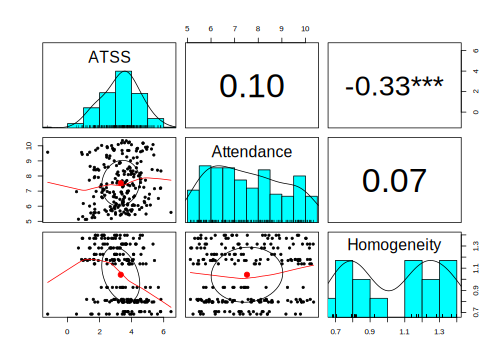
\includegraphics{ReC_Multilevel_files/figure-latex/pairs panels of MLM variables-1.pdf}
What do we observe in this preliminary, zero-ordered relationship?

\begin{itemize}
\tightlist
\item
  As racial homogeneity increases, homonegativity decreases.

  \begin{itemize}
  \tightlist
  \item
    Curiously, there is a non-linear curve between those two variables -- but that seems to be ``pulled'' by an outlier(?) in the lower right quandrant of the ATSS/Homonegativity relationship.
  \end{itemize}
\item
  ATTS appears to be normally distributed
\item
  Attendance has a flat distribution
\end{itemize}

We can learn more by examining descriptive statistics.

\begin{Shaded}
\begin{Highlighting}[]
\NormalTok{psych}\SpecialCharTok{::}\FunctionTok{describe}\NormalTok{(Lefevor2020[}\FunctionTok{c}\NormalTok{(}\StringTok{"ATSS"}\NormalTok{, }\StringTok{"Attendance"}\NormalTok{, }\StringTok{"Homogeneity"}\NormalTok{)])}
\end{Highlighting}
\end{Shaded}

\begin{verbatim}
            vars   n mean   sd median trimmed  mad   min   max range  skew
ATSS           1 225 3.32 1.18   3.43    3.34 1.11 -1.23  6.45  7.69 -0.30
Attendance     2 225 7.52 1.52   7.36    7.47 1.84  5.12 10.35  5.22  0.24
Homogeneity    3 225 1.04 0.25   1.14    1.04 0.34  0.69  1.40  0.71 -0.04
            kurtosis   se
ATSS            0.27 0.08
Attendance     -1.19 0.10
Homogeneity    -1.60 0.02
\end{verbatim}

These descriptives allow us a glimpse of the means and standard deviations of our study variables. Additionally, we can look at skew and kurtosis to see that our variables are within the normal ranges (i.e., below 3 for skew; below 8 for kurtosis \citep{kline_principles_2016}).

\hypertarget{levels}{%
\subsection{Levels}\label{levels}}

\emph{Levels} are a critical component of MLM. In the context of MLM models of nesting within groups/clusters (e.g., cross-sectional MLM):

\begin{itemize}
\tightlist
\item
  Level 1 (L1) variables ``belong to the person''

  \begin{itemize}
  \tightlist
  \item
    Age, race, attitudinal or behavioral assessment
  \end{itemize}
\item
  Level 2 (L2) variables ``belong to the group/cluster''

  \begin{itemize}
  \tightlist
  \item
    Leader characteristic, economic indicator that is unique to the group/cluster
  \item
    Aggregate/composite representation of L1 variables
  \end{itemize}
\end{itemize}

In our tiny model from the Lefevor et al. \citeyearpar{lefevor_homonegativity_2020} vignette:

\begin{itemize}
\tightlist
\item
  ATSS/homonegativity is our DV; it is an L1 observation because we are predicting individual's attitudes toward same-sex sexuality.
\item
  Attendance is an L1 observation \emph{when} we are using it as the individual's own church attendance.
\item
  Attendance \emph{will be } an L2 observation when we aggregate it an use it as a value to represent the church.
\item
  Racial homogeneity is only entered as an L2 variable. It was collected at the individual level via self-identification of race and calculated to represent the proportion of Black individuals in the church.
\end{itemize}

\begin{Shaded}
\begin{Highlighting}[]
\FunctionTok{head}\NormalTok{(Lefevor2020[}\FunctionTok{c}\NormalTok{(}\StringTok{"church"}\NormalTok{, }\StringTok{"ATSS"}\NormalTok{, }\StringTok{"Attendance"}\NormalTok{, }\StringTok{"Homogeneity"}\NormalTok{)], }\AttributeTok{n =}\NormalTok{ 30L)}
\end{Highlighting}
\end{Shaded}

\begin{verbatim}
   church      ATSS Attendance Homogeneity
1       A 4.7835442   6.318674   0.7957395
2       A 5.3851521   9.391428   0.7957395
3       A 4.3722317   9.832894   0.7957395
4       A 4.8635210   7.721731   0.7957395
5       A 4.9733886   9.917289   0.7957395
6       A 4.3455429   8.844333   0.7957395
7       A 3.5357514   6.630585   0.7957395
8       A 4.1572480   8.111701   0.7957395
9       A 4.2946421   9.658424   0.7957395
10      A 3.9311877   5.743799   0.7957395
11      A 4.9380802   6.048393   0.7957395
12      A 4.6318423   5.908200   0.7957395
13      A 3.4139728   7.685524   0.7957395
14      A 2.6348562   6.900703   0.7957395
15      A 4.8415811   6.594790   0.7957395
16      B 0.9835024   6.176724   1.1691398
17      B 1.9247771   7.907341   1.1691398
18      B 3.7576164   5.469059   1.1691398
19      B 3.6992782   9.262913   1.1691398
20      B 2.9125454   9.001514   1.1691398
21      B 4.0568240   7.486189   1.1691398
22      B 1.2471085   9.417031   1.1691398
23      B 3.2280375   6.066014   1.1691398
24      B 3.7688923   7.413705   1.1691398
25      B 4.0418646   6.047803   1.1691398
26      B 5.4240898   7.157878   1.1691398
27      B 3.8355654   9.687518   1.1691398
28      B 2.6657722   5.972512   1.1691398
29      B 2.8502831   9.761905   1.1691398
30      B 2.8982202   9.689345   1.1691398
\end{verbatim}

In this display of the first 30 rows, we see the data for the first two churches (i.e., A and B). The value is (potentially) different for each individual in each church for the two L1 variables: \emph{ATSS}, \emph{Attendance.} In contrast, the value of the variable is constant for the L2 variable, \emph{Homogeneity} for churches A and B.

\hypertarget{centering}{%
\subsection{Centering}\label{centering}}

Before we continue with modeling, we need to consider \emph{centering}. That is, we transform our predictor variables to give the intercept parameters more useful interpretations.

While there are some general practices, there are often arguments for different approaches:

\begin{itemize}
\tightlist
\item
  We usually focus centering on L1 predictors.
\item
  We usually focus centering on continuously scaled variables.
\item
  Dichotomous variables are considered to be centered, so long as there is a meaningful 0 (e.g., control group = 0; treatment group = 1), many do not further center.

  \begin{itemize}
  \tightlist
  \item
    Newsom \citeyearpar{newsom_centering_2019}, though, argues that if a binary variable is an L1 predictor, group mean centering produces intercepts weighted by the proportion of 1 to 0 values for each group; grand mean centering provides the sample weight adjustment to make the sample mean (each group's mean) proportionate to the population (full sample)
  \end{itemize}
\item
  Dependent variables are generally not centered
\end{itemize}

we generally consider three centering strategies:

The \textbf{natural metric} is ideal if the variable has a meaningful zero point (e.g., drug dosage, time). It is more difficult when there is a non-zero metric. When there are dichotomous variables, the natural metric works well (i.e., 0 = control group, 1 = treatment group). The natural metric is an acceptable choice when the interest is only on the effects of L1 variables, rather than on the effects of group-level variables.

\textbf{Grand mean centering (GCM)} involves subtracting the mean from each case's score on the variable. The intercept is interpreted as the expected value of the DV for a person/group that is compared with all individuals/groups.

\begin{itemize}
\tightlist
\item
  Intercepts are adjusted group means (like an ANCOVA model)
\item
  Variance in the intercepts represents between-group variance in the adjusted means (i.e., adjusted for L1 predictors)
\item
  The effects of L1 predictors are partialed out (controlled for) of the between-group variance
\item
  GCM is most useful when we are interested in

  \begin{itemize}
  \tightlist
  \item
    L2 predictors with L1 covariates
  \item
    Interactions specified L2
  \end{itemize}
\item
  GCM is a good choice when the primary interest is on the effects of L2 variables, controlling for the L1 predictors.
\end{itemize}

\textbf{Group mean centering} or \textbf{Centering within Context (CWC)} involves subtracting the mean of the individual's group from each score. The L1 intercept is interpreted as the expected mean on the DV for the person's group. Group mean centering/CWC:

\begin{itemize}
\tightlist
\item
  Provides a measure of the IV that accounts for one's relative standing within the group
\item
  Removes between-group variability from the model (deviations rom the group means are now the predictors)

  \begin{itemize}
  \tightlist
  \item
    If we only use group mean centering (CWC), we lose information about between-group differences
  \end{itemize}
\item
  Assumes that relative standing within the group is an important factor
\item
  Is most useful when we are interested in

  \begin{itemize}
  \tightlist
  \item
    Relations among L1 variables
  \item
    Interactions among L1 variables
  \item
    Interactions between L1 and L2 variables
  \end{itemize}
\item
  CWC is an acceptable choice when the interest is only on the effects of L1 variables, rather than on the effects of group-level variables because it provides unbiased estimates of the pooled within group effect of an individual variable.
\end{itemize}

In the case of making centering choices with our variables, we are must think about the \emph{frog pond effect}. That is, for the same size frog, the experience of being in a pond with big frogs may be different from being in a pond with small frogs. When we consider our present research vignette, we might ask,

\begin{itemize}
\tightlist
\item
  Does the effect of church attendance on ATSS depend only on the individual's own church attendance. Or,
\item
  Does the overall church attendance (``size'' of the pond) also related to ATSS?
\end{itemize}

\textbf{Compositional effects} \citep{enders_centering_2007} involves transforming the natural metric of the score into a group-mean centered (CWC) variable at L1 and a group mean \textbf{aggregate} at L2. Both the CWC/L1 and aggregate/L2 are entered into the MLM.

\begin{itemize}
\tightlist
\item
  When the aggregate is added back in at L2, we get \emph{direct} estimates of both the within- and between- group effects through group-mean centering
\item
  We term it \emph{compositional effects} because it represents the difference between the contextual-level effect and the person-level predictor.
\item
  This is a great strategy when the interest is on distinguishing individual effects of variables (e.g., church attendance) from group-level effects of that same variable (e.g., overall church attendance).
\end{itemize}

Following the Lefevor and colleagues' \citeyearpar{lefevor_homonegativity_2020} example, we will use the \emph{compositional effects} approach with our data. The \emph{group.center()} function in the R package, \emph{robumeta} will group mean center (CWC) variables. All we need to do is identify the clustering variable in our case, ``church.''

Similarly, \emph{robumeta}'s \emph{group.mean} function will aggregate variables at the group's mean.

\begin{Shaded}
\begin{Highlighting}[]
\FunctionTok{library}\NormalTok{(robumeta)}
\NormalTok{Lefevor2020}\SpecialCharTok{$}\NormalTok{AttendL1 }\OtherTok{\textless{}{-}} \FunctionTok{as.numeric}\NormalTok{(}\FunctionTok{group.center}\NormalTok{(Lefevor2020}\SpecialCharTok{$}\NormalTok{Attendance, Lefevor2020}\SpecialCharTok{$}\NormalTok{church))}\CommentTok{\#centered within context (group mean centering)}
\NormalTok{Lefevor2020}\SpecialCharTok{$}\NormalTok{AttendL2 }\OtherTok{\textless{}{-}} \FunctionTok{as.numeric}\NormalTok{(}\FunctionTok{group.mean}\NormalTok{(Lefevor2020}\SpecialCharTok{$}\NormalTok{Attendance, Lefevor2020}\SpecialCharTok{$}\NormalTok{church))}\CommentTok{\#aggregated at group mean}
\end{Highlighting}
\end{Shaded}

\begin{Shaded}
\begin{Highlighting}[]
\FunctionTok{head}\NormalTok{(Lefevor2020[}\FunctionTok{c}\NormalTok{(}\StringTok{"church"}\NormalTok{, }\StringTok{"ATSS"}\NormalTok{, }\StringTok{"Attendance"}\NormalTok{, }\StringTok{"AttendL1"}\NormalTok{, }\StringTok{"AttendL2"}\NormalTok{, }\StringTok{"Homogeneity"}\NormalTok{)], }\AttributeTok{n =}\NormalTok{ 30L)}
\end{Highlighting}
\end{Shaded}

\begin{verbatim}
   church      ATSS Attendance     AttendL1 AttendL2 Homogeneity
1       A 4.7835442   6.318674 -1.368556846 7.687231   0.7957395
2       A 5.3851521   9.391428  1.704196481 7.687231   0.7957395
3       A 4.3722317   9.832894  2.145662408 7.687231   0.7957395
4       A 4.8635210   7.721731  0.034499326 7.687231   0.7957395
5       A 4.9733886   9.917289  2.230057976 7.687231   0.7957395
6       A 4.3455429   8.844333  1.157102115 7.687231   0.7957395
7       A 3.5357514   6.630585 -1.056646112 7.687231   0.7957395
8       A 4.1572480   8.111701  0.424469781 7.687231   0.7957395
9       A 4.2946421   9.658424  1.971192960 7.687231   0.7957395
10      A 3.9311877   5.743799 -1.943432538 7.687231   0.7957395
11      A 4.9380802   6.048393 -1.638837820 7.687231   0.7957395
12      A 4.6318423   5.908200 -1.779031167 7.687231   0.7957395
13      A 3.4139728   7.685524 -0.001707147 7.687231   0.7957395
14      A 2.6348562   6.900703 -0.786528003 7.687231   0.7957395
15      A 4.8415811   6.594790 -1.092441414 7.687231   0.7957395
16      B 0.9835024   6.176724 -1.591106297 7.767830   1.1691398
17      B 1.9247771   7.907341  0.139510679 7.767830   1.1691398
18      B 3.7576164   5.469059 -2.298771340 7.767830   1.1691398
19      B 3.6992782   9.262913  1.495083015 7.767830   1.1691398
20      B 2.9125454   9.001514  1.233683676 7.767830   1.1691398
21      B 4.0568240   7.486189 -0.281641399 7.767830   1.1691398
22      B 1.2471085   9.417031  1.649200996 7.767830   1.1691398
23      B 3.2280375   6.066014 -1.701816135 7.767830   1.1691398
24      B 3.7688923   7.413705 -0.354124518 7.767830   1.1691398
25      B 4.0418646   6.047803 -1.720027268 7.767830   1.1691398
26      B 5.4240898   7.157878 -0.609951815 7.767830   1.1691398
27      B 3.8355654   9.687518  1.919687868 7.767830   1.1691398
28      B 2.6657722   5.972512 -1.795317977 7.767830   1.1691398
29      B 2.8502831   9.761905  1.994075223 7.767830   1.1691398
30      B 2.8982202   9.689345  1.921515292 7.767830   1.1691398
\end{verbatim}

If we look again at the first two churches, we can see the

\begin{itemize}
\tightlist
\item
  Natural metric (ATSS, Attendance) which differs for each person across all churches

  \begin{itemize}
  \tightlist
  \item
    This would be an L1 variable
  \end{itemize}
\item
  Group-mean centering (CWC; ATSSL2) which is identifiable because if you added up each of the values in each of the churches, the sum would be zero for each church

  \begin{itemize}
  \tightlist
  \item
    This would be an L1 variable
  \end{itemize}
\item
  Aggregate group mean (AttendL2) which is identifiable because the value is constant across each of the groups

  \begin{itemize}
  \tightlist
  \item
    This would be an L2 variable
  \end{itemize}
\item
  You might notice, I didn't mention the \emph{homogeneity} variable. This is because it was collected and entered as an L2 variable and needs no further centering/transformation. Similarly, we typically leave the dependent variable (\emph{ATSS}) in the natural metric.
\end{itemize}

We can also see the effects of centering in our descriptives.

\begin{Shaded}
\begin{Highlighting}[]
\NormalTok{psych}\SpecialCharTok{::}\FunctionTok{describe}\NormalTok{(Lefevor2020[}\FunctionTok{c}\NormalTok{(}\StringTok{"ATSS"}\NormalTok{, }\StringTok{"Attendance"}\NormalTok{, }\StringTok{"AttendL1"}\NormalTok{, }\StringTok{"AttendL2"}\NormalTok{, }\StringTok{"Homogeneity"}\NormalTok{)])}
\end{Highlighting}
\end{Shaded}

\begin{verbatim}
            vars   n mean   sd median trimmed  mad   min   max range  skew
ATSS           1 225 3.32 1.18   3.43    3.34 1.11 -1.23  6.45  7.69 -0.30
Attendance     2 225 7.52 1.52   7.36    7.47 1.84  5.12 10.35  5.22  0.24
AttendL1       3 225 0.00 1.48  -0.01   -0.02 1.88 -2.93  3.01  5.94  0.10
AttendL2       4 225 7.52 0.32   7.55    7.52 0.33  7.01  8.06  1.05  0.02
Homogeneity    5 225 1.04 0.25   1.14    1.04 0.34  0.69  1.40  0.71 -0.04
            kurtosis   se
ATSS            0.27 0.08
Attendance     -1.19 0.10
AttendL1       -1.14 0.10
AttendL2       -0.93 0.02
Homogeneity    -1.60 0.02
\end{verbatim}

Note that the mean for the ATTSL1 and AttendL1 variables are now zero, while the aggregated group means are equal to the mean of the natural metric.

Looking at the descriptives for each church also helps clarify what we have done.

\begin{Shaded}
\begin{Highlighting}[]
\NormalTok{psych}\SpecialCharTok{::}\FunctionTok{describeBy}\NormalTok{(ATSS }\SpecialCharTok{+}\NormalTok{ Attendance }\SpecialCharTok{+}\NormalTok{ AttendL1 }\SpecialCharTok{+}\NormalTok{ AttendL2 }\SpecialCharTok{+}\NormalTok{ Homogeneity }\SpecialCharTok{\textasciitilde{}}\NormalTok{ church, }\AttributeTok{data =}\NormalTok{ Lefevor2020)}
\end{Highlighting}
\end{Shaded}

\begin{verbatim}
 Descriptive statistics by group 
church: A
            vars  n mean   sd median trimmed  mad   min  max range  skew
ATSS           1 15 4.34 0.72   4.37    4.39 0.70  2.63 5.39  2.75 -0.78
Attendance     2 15 7.69 1.52   7.69    7.67 2.03  5.74 9.92  4.17  0.23
AttendL1       3 15 0.00 1.52   0.00   -0.02 2.03 -1.94 2.23  4.17  0.23
AttendL2       4 15 7.69 0.00   7.69    7.69 0.00  7.69 7.69  0.00   NaN
Homogeneity    5 15 0.80 0.00   0.80    0.80 0.00  0.80 0.80  0.00   NaN
            kurtosis   se
ATSS           -0.21 0.19
Attendance     -1.63 0.39
AttendL1       -1.63 0.39
AttendL2         NaN 0.00
Homogeneity      NaN 0.00
------------------------------------------------------------ 
church: B
            vars  n mean   sd median trimmed  mad   min  max range  skew
ATSS           1 15 3.15 1.15   3.23    3.15 0.83  0.98 5.42  4.44 -0.22
Attendance     2 15 7.77 1.59   7.49    7.79 2.24  5.47 9.76  4.29 -0.01
AttendL1       3 15 0.00 1.59  -0.28    0.02 2.24 -2.30 1.99  4.29 -0.01
AttendL2       4 15 7.77 0.00   7.77    7.77 0.00  7.77 7.77  0.00   NaN
Homogeneity    5 15 1.17 0.00   1.17    1.17 0.00  1.17 1.17  0.00   NaN
            kurtosis   se
ATSS           -0.50 0.30
Attendance     -1.75 0.41
AttendL1       -1.75 0.41
AttendL2         NaN 0.00
Homogeneity      NaN 0.00
------------------------------------------------------------ 
church: C
            vars  n mean   sd median trimmed  mad   min  max range skew
ATSS           1 15 2.93 0.92   2.98    2.90 1.14  1.68 4.58  2.91 0.14
Attendance     2 15 7.01 1.01   6.78    6.95 0.87  5.83 8.96  3.13 0.75
AttendL1       3 15 0.00 1.01  -0.22   -0.06 0.87 -1.18 1.95  3.13 0.75
AttendL2       4 15 7.01 0.00   7.01    7.01 0.00  7.01 7.01  0.00  NaN
Homogeneity    5 15 1.22 0.00   1.22    1.22 0.00  1.22 1.22  0.00  NaN
            kurtosis   se
ATSS           -1.20 0.24
Attendance     -0.88 0.26
AttendL1       -0.88 0.26
AttendL2         NaN 0.00
Homogeneity      NaN 0.00
------------------------------------------------------------ 
church: D
            vars  n mean   sd median trimmed  mad   min   max range  skew
ATSS           1 15 2.62 1.07   2.79    2.64 1.43  0.88  4.10  3.22 -0.21
Attendance     2 15 8.06 1.85   8.41    8.12 2.27  5.12 10.20  5.08 -0.29
AttendL1       3 15 0.00 1.85   0.36    0.06 2.27 -2.93  2.14  5.08 -0.29
AttendL2       4 15 8.06 0.00   8.06    8.06 0.00  8.06  8.06  0.00   NaN
Homogeneity    5 15 1.18 0.00   1.18    1.18 0.00  1.18  1.18  0.00   NaN
            kurtosis   se
ATSS           -1.54 0.28
Attendance     -1.71 0.48
AttendL1       -1.71 0.48
AttendL2         NaN 0.00
Homogeneity      NaN 0.00
------------------------------------------------------------ 
church: E
            vars  n mean   sd median trimmed  mad   min   max range  skew
ATSS           1 15 3.42 0.92   3.57    3.41 0.49  1.70  5.33  3.63 -0.05
Attendance     2 15 8.00 1.70   7.95    8.02 2.27  5.50 10.33  4.82 -0.01
AttendL1       3 15 0.00 1.70  -0.05    0.01 2.27 -2.50  2.32  4.82 -0.01
AttendL2       4 15 8.00 0.00   8.00    8.00 0.00  8.00  8.00  0.00   NaN
Homogeneity    5 15 1.32 0.00   1.32    1.32 0.00  1.32  1.32  0.00   NaN
            kurtosis   se
ATSS           -0.49 0.24
Attendance     -1.56 0.44
AttendL1       -1.56 0.44
AttendL2         NaN 0.00
Homogeneity      NaN 0.00
------------------------------------------------------------ 
church: F
            vars  n mean   sd median trimmed  mad   min  max range skew
ATSS           1 15 3.61 1.04   3.44    3.57 0.96  2.11 5.67  3.56 0.46
Attendance     2 15 7.27 1.18   7.27    7.19 1.04  5.68 9.90  4.22 0.69
AttendL1       3 15 0.00 1.18   0.00   -0.08 1.04 -1.59 2.63  4.22 0.69
AttendL2       4 15 7.27 0.00   7.27    7.27 0.00  7.27 7.27  0.00  NaN
Homogeneity    5 15 0.93 0.00   0.93    0.93 0.00  0.93 0.93  0.00  NaN
            kurtosis   se
ATSS           -0.95 0.27
Attendance     -0.33 0.30
AttendL1       -0.33 0.30
AttendL2         NaN 0.00
Homogeneity      NaN 0.00
------------------------------------------------------------ 
church: G
            vars  n mean   sd median trimmed  mad   min  max range  skew
ATSS           1 15 4.51 0.94   4.49    4.44 1.08  3.48 6.45  2.98  0.65
Attendance     2 15 7.01 0.94   7.18    7.01 1.27  5.50 8.47  2.96 -0.05
AttendL1       3 15 0.00 0.94   0.17    0.00 1.27 -1.50 1.46  2.96 -0.05
AttendL2       4 15 7.01 0.00   7.01    7.01 0.00  7.01 7.01  0.00   NaN
Homogeneity    5 15 0.71 0.00   0.71    0.71 0.00  0.71 0.71  0.00   NaN
            kurtosis   se
ATSS           -0.94 0.24
Attendance     -1.35 0.24
AttendL1       -1.35 0.24
AttendL2         NaN 0.00
Homogeneity      NaN 0.00
------------------------------------------------------------ 
church: H
            vars  n mean   sd median trimmed  mad   min   max range  skew
ATSS           1 15 3.55 1.19   3.48    3.55 0.84  1.20  5.83  4.63 -0.17
Attendance     2 15 7.35 1.70   7.57    7.30 2.45  5.13 10.20  5.07  0.23
AttendL1       3 15 0.00 1.70   0.22   -0.05 2.45 -2.22  2.86  5.07  0.23
AttendL2       4 15 7.35 0.00   7.35    7.35 0.00  7.35  7.35  0.00   NaN
Homogeneity    5 15 0.82 0.00   0.82    0.82 0.00  0.82  0.82  0.00   NaN
            kurtosis   se
ATSS           -0.43 0.31
Attendance     -1.46 0.44
AttendL1       -1.46 0.44
AttendL2         NaN 0.00
Homogeneity      NaN 0.00
------------------------------------------------------------ 
church: I
            vars  n mean   sd median trimmed  mad   min   max range skew
ATSS           1 15 2.71 1.13   2.73    2.71 0.83  0.68  4.76  4.08 0.16
Attendance     2 15 7.26 1.63   7.25    7.20 2.26  5.14 10.17  5.03 0.12
AttendL1       3 15 0.00 1.63  -0.01   -0.06 2.26 -2.12  2.90  5.03 0.12
AttendL2       4 15 7.26 0.00   7.26    7.26 0.00  7.26  7.26  0.00  NaN
Homogeneity    5 15 1.28 0.00   1.28    1.28 0.00  1.28  1.28  0.00  NaN
            kurtosis   se
ATSS           -0.61 0.29
Attendance     -1.43 0.42
AttendL1       -1.43 0.42
AttendL2         NaN 0.00
Homogeneity      NaN 0.00
------------------------------------------------------------ 
church: J
            vars  n mean   sd median trimmed  mad   min   max range  skew
ATSS           1 15 3.47 0.99   3.81    3.50 1.05  1.67  4.90  3.23 -0.44
Attendance     2 15 7.86 1.89   7.89    7.88 2.89  5.25 10.25  5.00 -0.09
AttendL1       3 15 0.00 1.89   0.03    0.02 2.89 -2.62  2.39  5.00 -0.09
AttendL2       4 15 7.86 0.00   7.86    7.86 0.00  7.86  7.86  0.00   NaN
Homogeneity    5 15 1.14 0.00   1.14    1.14 0.00  1.14  1.14  0.00   NaN
            kurtosis   se
ATSS           -0.94 0.26
Attendance     -1.70 0.49
AttendL1       -1.70 0.49
AttendL2         NaN 0.00
Homogeneity      NaN 0.00
------------------------------------------------------------ 
church: K
            vars  n mean   sd median trimmed  mad   min   max range skew
ATSS           1 15 2.45 1.04   2.53    2.41 1.09  0.92  4.49  3.57 0.30
Attendance     2 15 7.43 1.83   6.73    7.40 2.10  5.31 10.03  4.72 0.15
AttendL1       3 15 0.00 1.83  -0.71   -0.04 2.10 -2.12  2.59  4.72 0.15
AttendL2       4 15 7.43 0.00   7.43    7.43 0.00  7.43  7.43  0.00  NaN
Homogeneity    5 15 1.37 0.00   1.37    1.37 0.00  1.37  1.37  0.00  NaN
            kurtosis   se
ATSS           -0.82 0.27
Attendance     -1.81 0.47
AttendL1       -1.81 0.47
AttendL2         NaN 0.00
Homogeneity      NaN 0.00
------------------------------------------------------------ 
church: L
            vars  n mean   sd median trimmed  mad   min  max range skew
ATSS           1 15 2.87 0.95   2.94    2.82 1.12  1.73 4.67  2.94  0.5
Attendance     2 15 7.68 1.27   7.54    7.69 1.36  5.57 9.71  4.14  0.1
AttendL1       3 15 0.00 1.27  -0.15    0.01 1.36 -2.11 2.03  4.14  0.1
AttendL2       4 15 7.68 0.00   7.68    7.68 0.00  7.68 7.68  0.00  NaN
Homogeneity    5 15 1.40 0.00   1.40    1.40 0.00  1.40 1.40  0.00  NaN
            kurtosis   se
ATSS           -1.06 0.25
Attendance     -1.33 0.33
AttendL1       -1.33 0.33
AttendL2         NaN 0.00
Homogeneity      NaN 0.00
------------------------------------------------------------ 
church: M
            vars  n mean   sd median trimmed  mad   min   max range  skew
ATSS           1 15 3.72 0.79   3.93    3.72 0.73  2.34  5.06  2.72 -0.27
Attendance     2 15 7.56 1.52   7.80    7.52 1.94  5.45 10.07  4.63  0.12
AttendL1       3 15 0.00 1.52   0.25   -0.03 1.94 -2.11  2.52  4.63  0.12
AttendL2       4 15 7.56 0.00   7.56    7.56 0.00  7.56  7.56  0.00   NaN
Homogeneity    5 15 0.81 0.00   0.81    0.81 0.00  0.81  0.81  0.00   NaN
            kurtosis   se
ATSS           -1.06 0.20
Attendance     -1.42 0.39
AttendL1       -1.42 0.39
AttendL2         NaN 0.00
Homogeneity      NaN 0.00
------------------------------------------------------------ 
church: N
            vars  n mean   sd median trimmed  mad   min  max range  skew
ATSS           1 15 2.82 1.79   3.11    2.91 1.51 -1.23 5.61  6.84 -0.48
Attendance     2 15 7.55 1.44   7.66    7.55 1.08  5.24 9.79  4.55 -0.10
AttendL1       3 15 0.00 1.44   0.11    0.01 1.08 -2.31 2.24  4.55 -0.10
AttendL2       4 15 7.55 0.00   7.55    7.55 0.00  7.55 7.55  0.00   NaN
Homogeneity    5 15 0.69 0.00   0.69    0.69 0.00  0.69 0.69  0.00   NaN
            kurtosis   se
ATSS           -0.38 0.46
Attendance     -1.27 0.37
AttendL1       -1.27 0.37
AttendL2         NaN 0.00
Homogeneity      NaN 0.00
------------------------------------------------------------ 
church: O
            vars  n mean   sd median trimmed  mad   min   max range  skew
ATSS           1 15 3.65 0.91   3.75    3.67 0.63  1.71  5.28  3.57 -0.67
Attendance     2 15 7.34 1.53   6.68    7.23 1.31  5.70 10.35  4.64  0.58
AttendL1       3 15 0.00 1.53  -0.65   -0.11 1.31 -1.63  3.01  4.64  0.58
AttendL2       4 15 7.34 0.00   7.34    7.34 0.00  7.34  7.34  0.00   NaN
Homogeneity    5 15 0.79 0.00   0.79    0.79 0.00  0.79  0.79  0.00   NaN
            kurtosis   se
ATSS            0.11 0.23
Attendance     -1.16 0.40
AttendL1       -1.16 0.40
AttendL2         NaN 0.00
Homogeneity      NaN 0.00
\end{verbatim}

Tables are produced for each church's data. Again, because of group-mean centering (CWC) the mean of the ATSSL1 and AttendL1 variables are 0. The values of the ATSSL2 and AttendL1 variables equal the natural metric. These, though, are different for each of the churches.

Looking at the correlations between all forms of these variables can further help clarify why the \emph{compositional effects} approach is useful.

\begin{Shaded}
\begin{Highlighting}[]
\CommentTok{\#Multilevel level correlation matrix}
\NormalTok{apaTables}\SpecialCharTok{::}\FunctionTok{apa.cor.table}\NormalTok{(Lefevor2020[}\FunctionTok{c}\NormalTok{(}
\StringTok{"ATSS"}\NormalTok{, }\StringTok{"Attendance"}\NormalTok{, }\StringTok{"AttendL1"}\NormalTok{, }\StringTok{"AttendL2"}\NormalTok{, }\StringTok{"Homogeneity"}\NormalTok{)], }\AttributeTok{show.conf.interval =} \ConstantTok{FALSE}\NormalTok{, }\AttributeTok{landscape =} \ConstantTok{TRUE}\NormalTok{, }\AttributeTok{table.number =} \DecValTok{1}\NormalTok{, }\AttributeTok{filename=}\StringTok{"ML\_CorMatrix.doc"}\NormalTok{)}
\end{Highlighting}
\end{Shaded}

\begin{verbatim}
The ability to suppress reporting of reporting confidence intervals has been deprecated in this version.
The function argument show.conf.interval will be removed in a later version.
\end{verbatim}

\begin{verbatim}

Table 1 

Means, standard deviations, and correlations with confidence intervals
 

  Variable       M     SD   1            2           3           4         
  1. ATSS        3.32  1.18                                                
                                                                           
  2. Attendance  7.52  1.52 .10                                            
                            [-.03, .23]                                    
                                                                           
  3. AttendL1    -0.00 1.48 .12          .98**                             
                            [-.01, .25]  [.97, .98]                        
                                                                           
  4. AttendL2    7.52  0.32 -.10         .21**       -.00                  
                            [-.23, .03]  [.08, .33]  [-.13, .13]           
                                                                           
  5. Homogeneity 1.04  0.25 -.33**       .07         -.00        .32**     
                            [-.44, -.21] [-.07, .19] [-.13, .13] [.19, .43]
                                                                           

Note. M and SD are used to represent mean and standard deviation, respectively.
Values in square brackets indicate the 95% confidence interval.
The confidence interval is a plausible range of population correlations 
that could have caused the sample correlation (Cumming, 2014).
 * indicates p < .05. ** indicates p < .01.
 
\end{verbatim}

The AttendL2 (aggregated group means) we created correlates with the Attendance (natural metric) version. However, it has ZERO correlation with the AttendL1 (group-mean centered, CWC) version. This means that it effectively and completely separates within- and between-subjects variance. If we enter these both into the MLM prediction equation, we will completely capture the within- and between-subjects contributions of attendance.

The compositional effects approach to representing L1 variables also works well with longitudinal MLM.

\hypertarget{model-building}{%
\subsection{Model Building}\label{model-building}}

Multilevel modelers often approach model building in a systematic and sequential manner. This approach was true for Lefevor and colleagues \citeyearpar{lefevor_homonegativity_2020} who planned a four staged approach, but stopped after three because it appeared that adding the next term would not result in model improvement. The four planned steps include:

\begin{itemize}
\tightlist
\item
  Examining an intercept-only model
\item
  Adding the L1 variables
\item
  Adding the L2 variables
\item
  Adding cross-level interactions
\end{itemize}

\hypertarget{model-1-the-empty-model}{%
\subsubsection{\texorpdfstring{Model 1: The \emph{empty} model}{Model 1: The empty model}}\label{model-1-the-empty-model}}

This preliminary model has several names: unconditional cell means model, one-way ANOVA with random effects, intercept-only model, and empty model. Why? The only variable in the model is the DV. That is, it is a model with no predictors.

As you can see in the script below, we are specifying its intercept (\textasciitilde1). The ``\emph{(1 \textbar{} church)}'' portion of the code indicates there is a random intercept with a fixed mean. That is, the formula acknowledges that the ATSS means will differ across churches. This model will have no slope. That is, each individual score is predicted solely from the mean. In another lecture, I talk about the transition from null hypothesis statistical testing to statistical modeling. In that lecture I reflected on Cumming's \citeyearpar{cumming_new_2014} notion that ``even the mean is a model'' -- that it explains something and not others. In this circumstance, the mean is a model! What is, perhaps, unique about this model is that the code below allows the mean to vary across groups.

There are two packages (\emph{lme4}, \emph{nlme}) that are primarily used for MLM. We are providing the code for both because -- although the core features are identical -- they are slightly different. The \emph{lmerTest} package offers some handy follow-up tests that help us understand our results. Finally, the \emph{tab\_model()} function from the \emph{sjPlot} package will help create a table that is readily usable in an APA style journal article.

\begin{Shaded}
\begin{Highlighting}[]
\FunctionTok{library}\NormalTok{(lme4)}
\NormalTok{Mod1 }\OtherTok{\textless{}{-}} \FunctionTok{lmer}\NormalTok{(ATSS }\SpecialCharTok{\textasciitilde{}}\DecValTok{1} \SpecialCharTok{+}\NormalTok{ (}\DecValTok{1} \SpecialCharTok{|}\NormalTok{ church), }\AttributeTok{REML =} \ConstantTok{FALSE}\NormalTok{, }\AttributeTok{data =}\NormalTok{ Lefevor2020)}
\FunctionTok{summary}\NormalTok{(Mod1)}
\end{Highlighting}
\end{Shaded}

\begin{verbatim}
Linear mixed model fit by maximum likelihood . t-tests use Satterthwaite's
  method [lmerModLmerTest]
Formula: ATSS ~ 1 + (1 | church)
   Data: Lefevor2020

     AIC      BIC   logLik deviance df.resid 
   694.7    705.0   -344.4    688.7      222 

Scaled residuals: 
    Min      1Q  Median      3Q     Max 
-3.9130 -0.6410  0.0392  0.5764  2.5252 

Random effects:
 Groups   Name        Variance Std.Dev.
 church   (Intercept) 0.2673   0.5171  
 Residual             1.1299   1.0630  
Number of obs: 225, groups:  church, 15

Fixed effects:
            Estimate Std. Error      df t value          Pr(>|t|)    
(Intercept)   3.3214     0.1511 15.0000   21.98 0.000000000000803 ***
---
Signif. codes:  0 '***' 0.001 '**' 0.01 '*' 0.05 '.' 0.1 ' ' 1
\end{verbatim}

\begin{Shaded}
\begin{Highlighting}[]
\FunctionTok{AIC}\NormalTok{(Mod1) }\CommentTok{\# request AIC}
\end{Highlighting}
\end{Shaded}

\begin{verbatim}
[1] 694.73
\end{verbatim}

\begin{Shaded}
\begin{Highlighting}[]
\FunctionTok{BIC}\NormalTok{(Mod1) }\CommentTok{\# request BIC}
\end{Highlighting}
\end{Shaded}

\begin{verbatim}
[1] 704.9783
\end{verbatim}

\begin{Shaded}
\begin{Highlighting}[]
\FunctionTok{library}\NormalTok{(nlme)}
\end{Highlighting}
\end{Shaded}

\begin{verbatim}
Attaching package: 'nlme'
\end{verbatim}

\begin{verbatim}
The following object is masked from 'package:dplyr':

    collapse
\end{verbatim}

\begin{verbatim}
The following object is masked from 'package:lme4':

    lmList
\end{verbatim}

\begin{Shaded}
\begin{Highlighting}[]
\NormalTok{ModB1 }\OtherTok{\textless{}{-}} \FunctionTok{lme}\NormalTok{(ATSS }\SpecialCharTok{\textasciitilde{}} \DecValTok{1}\NormalTok{, }\AttributeTok{random =} \SpecialCharTok{\textasciitilde{}} \DecValTok{1}\SpecialCharTok{|}\NormalTok{church, }\AttributeTok{method=}\StringTok{"ML"}\NormalTok{, }\AttributeTok{na.action =}\NormalTok{ na.omit, }\AttributeTok{data =}\NormalTok{ Lefevor2020)}
\FunctionTok{summary}\NormalTok{(ModB1)}
\end{Highlighting}
\end{Shaded}

\begin{verbatim}
Linear mixed-effects model fit by maximum likelihood
  Data: Lefevor2020 
     AIC      BIC   logLik
  694.73 704.9783 -344.365

Random effects:
 Formula: ~1 | church
        (Intercept) Residual
StdDev:   0.5170587 1.062978

Fixed effects:  ATSS ~ 1 
               Value Std.Error  DF  t-value p-value
(Intercept) 3.321371 0.1514833 210 21.92566       0

Standardized Within-Group Residuals:
        Min          Q1         Med          Q3         Max 
-3.91296264 -0.64096244  0.03922427  0.57637964  2.52520439 

Number of Observations: 225
Number of Groups: 15 
\end{verbatim}

\begin{Shaded}
\begin{Highlighting}[]
\FunctionTok{anova}\NormalTok{(ModB1) }\CommentTok{\# request F{-}tests for fixed effects}
\end{Highlighting}
\end{Shaded}

\begin{verbatim}
            numDF denDF  F-value p-value
(Intercept)     1   210 480.7347  <.0001
\end{verbatim}

\begin{Shaded}
\begin{Highlighting}[]
\FunctionTok{library}\NormalTok{(lmerTest)}
\FunctionTok{ranova}\NormalTok{(Mod1) }\CommentTok{\# request test of random effects}
\end{Highlighting}
\end{Shaded}

\begin{verbatim}
ANOVA-like table for random-effects: Single term deletions

Model:
ATSS ~ (1 | church)
             npar  logLik    AIC   LRT Df   Pr(>Chisq)    
<none>          3 -344.37 694.73                          
(1 | church)    2 -356.89 717.79 25.06  1 0.0000005558 ***
---
Signif. codes:  0 '***' 0.001 '**' 0.01 '*' 0.05 '.' 0.1 ' ' 1
\end{verbatim}

\begin{Shaded}
\begin{Highlighting}[]
\FunctionTok{confint}\NormalTok{(Mod1) }\CommentTok{\# request test of random effects (variance displayed as SD)}
\end{Highlighting}
\end{Shaded}

\begin{verbatim}
Computing profile confidence intervals ...
\end{verbatim}

\begin{verbatim}
                2.5 %    97.5 %
.sig01      0.3231248 0.8347723
.sigma      0.9688860 1.1733458
(Intercept) 3.0051108 3.6376320
\end{verbatim}

\begin{Shaded}
\begin{Highlighting}[]
\CommentTok{\# Extract Variances to compute R\^{}2}
\NormalTok{  var\_table }\OtherTok{=} \FunctionTok{as.data.frame}\NormalTok{(}\FunctionTok{VarCorr}\NormalTok{(Mod1))}
\NormalTok{  Mod1\_var\_tot }\OtherTok{=}\NormalTok{ var\_table[}\DecValTok{1}\NormalTok{,}\StringTok{\textquotesingle{}vcov\textquotesingle{}}\NormalTok{] }\SpecialCharTok{+}\NormalTok{ var\_table[}\DecValTok{2}\NormalTok{,}\StringTok{\textquotesingle{}vcov\textquotesingle{}}\NormalTok{] }\CommentTok{\# var\_table[1,\textquotesingle{}vcov\textquotesingle{}] = L1 var; var\_table[2,\textquotesingle{}vcov\textquotesingle{}] = L2 var;  }

\FunctionTok{library}\NormalTok{(sjPlot)}
\end{Highlighting}
\end{Shaded}

\begin{verbatim}
Warning: package 'sjPlot' was built under R version 4.0.5
\end{verbatim}

\begin{verbatim}
Learn more about sjPlot with 'browseVignettes("sjPlot")'.
\end{verbatim}

\begin{Shaded}
\begin{Highlighting}[]
\FunctionTok{tab\_model}\NormalTok{(Mod1, ModB1, }\AttributeTok{p.style =} \StringTok{"numeric"}\NormalTok{, }\AttributeTok{show.ci =} \ConstantTok{FALSE}\NormalTok{, }\AttributeTok{show.se =} \ConstantTok{TRUE}\NormalTok{, }\AttributeTok{show.df =} \ConstantTok{FALSE}\NormalTok{, }\AttributeTok{show.re.var =} \ConstantTok{TRUE}\NormalTok{, }\AttributeTok{show.aic =} \ConstantTok{TRUE}\NormalTok{, }\AttributeTok{show.dev =} \ConstantTok{TRUE}\NormalTok{, }\AttributeTok{use.viewer =} \ConstantTok{TRUE}\NormalTok{, }\AttributeTok{dv.labels =} \FunctionTok{c}\NormalTok{(}\StringTok{"Mod1"}\NormalTok{, }\StringTok{"ModB1"}\NormalTok{))}
\end{Highlighting}
\end{Shaded}

~

Mod1

ModB1

Predictors

Estimates

std. Error

p

Estimates

std. Error

p

(Intercept)

3.32

0.15

\textless0.001

3.32

0.15

\textless0.001

Random Effects

σ2

1.13

1.13

τ00

0.27 church

0.27 church

ICC

0.19

0.19

N

15 church

15 church

Observations

225

225

Marginal R2 / Conditional R2

0.000 / 0.191

0.000 / 0.191

Deviance

688.730

688.730

AIC

694.730

694.730

\begin{Shaded}
\begin{Highlighting}[]
\CommentTok{\#can swap this statement with the "file = "TabMod\_Table"" to get Viewer output or the outfile that you can open in Word}
\CommentTok{\#file = "TabMod\_Table.doc"}
\end{Highlighting}
\end{Shaded}

It is customary to report MLM models side-by-side for comparison. In this first run, I have extracted the intercept-only models from both the \emph{lmer()} and \emph{nlme()} runs to show that the results are identical. In subsequent runs, I will pull from the \emph{lmer()} models.

The unconditional cell means model is equivalent to a one-factor random effects ANOVA of attitudes toward same-sex sexuality as the sole factor; the 15 churches become the 15 levels of the churches factor.

With the \emph{plot\_model()} function in \emph{sjPlot}, we can plot the random effects. For this intercept-only model, we see the mean and range of the ATSS variable

\begin{Shaded}
\begin{Highlighting}[]
\FunctionTok{library}\NormalTok{(sjPlot)}
\NormalTok{sjPlot}\SpecialCharTok{::}\FunctionTok{plot\_model}\NormalTok{ (Mod1, }\AttributeTok{type=}\StringTok{"re"}\NormalTok{)}
\end{Highlighting}
\end{Shaded}

\begin{verbatim}
Warning in checkMatrixPackageVersion(): Package version inconsistency detected.
TMB was built with Matrix version 1.3.2
Current Matrix version is 1.2.18
Please re-install 'TMB' from source using install.packages('TMB', type = 'source') or ask CRAN for a binary version of 'TMB' matching CRAN's 'Matrix' package
\end{verbatim}

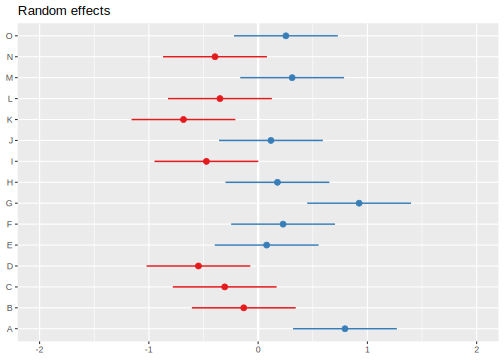
\includegraphics{ReC_Multilevel_files/figure-latex/unnamed-chunk-6-1.pdf}

Focusing on the information in viewer, we can first check to see if things look right. We know we have 15 churches, each with 15 observations (225), so our data is reading correctly.

The top of the output includes our \emph{fixed effects}. In this case, we have only the intercept, its standard error, and p value. We see that across all individuals in all churches, the mean (the grand mean) of ATSS is 3.32 (this is consistent with the \emph{M} we saw in descriptives). The values of fixed effects do not vary between L2 units. The \emph{tab\_model} viewer is very customizable; we can ask for different features.

The section of \emph{random effects} is different from OLS. Random effects include \emph{variance components}; these are reported here.

\(\sigma^{2}\) is within-church variance; the pooled scatter of each individual's response around the church's mean.
\(\tau _{00}\) is between-church variance; the scatter of each church's data around the grand mean.
The \emph{intraclass correlation coefficient} (ICC) describes the proportion of variance that lies \emph{between} churches. It is the essential piece of data that we need from this model. Because the total variation in \emph{Y} is just the sum of the within- and between- church variance components, we could have calculated this value from \(\sigma^{2}\) and \(\tau _{00}\). Yet, it is handy that the \emph{lmer()} function does it or us.

\begin{Shaded}
\begin{Highlighting}[]
\NormalTok{.}\DecValTok{27}\SpecialCharTok{/}\NormalTok{(}\FloatTok{1.13+.27}\NormalTok{)}
\end{Highlighting}
\end{Shaded}

\begin{verbatim}
[1] 0.1928571
\end{verbatim}

The ICC value of 0.19 means that 19\% of the total variation in attitudes toward same-sex sexuality is attributable to differences between churches. The balance\ldots{}

\begin{Shaded}
\begin{Highlighting}[]
\FloatTok{1.00} \SpecialCharTok{{-}}\NormalTok{ .}\DecValTok{19}
\end{Highlighting}
\end{Shaded}

\begin{verbatim}
[1] 0.81
\end{verbatim}

\ldots(81\%) is attributable to within-church variation (or differences in people).

We will monitor these variance components to see if the terms we have added reduce the variance. They can provide some sort of guide as to whether the remaining/unaccounted for variance is within-groups (where an L1 variable could help) or between-groups (where an L2 variable might be indicated). As they approach zero, it could be there is nothing left to explain.

\textbf{Marginal} \(R^2\) provides the variance provided only by the fixed effects.

\textbf{Conditional} \(R^2\) provides the variance provided by both the fixed and random effects (i.e., the mean random effect variances). Thus, the conditional \(R^2\) is appropriate or mixed models with random slopes or nested random effects. Already, without any predictors in the model, we have accounted for 19\% of the variance. How is this possible? Our empty model did include the clustering/nesting in churches. This is a random effect.

The \textbf{deviance statistic} compares log-likelihood statistics for two models at a time: (a) the current model and (b) a saturated model (e.g., a more general model that fits the sample data perfectly). Deviance quantifies \emph{how much worse} the current model is in comparison to the best possible model. The deviance is identical to the residual sums of squares used in regression. While you cannot directly interpret any particular deviance statistic, you can compare \emph{nested} models; the smaller value ``wins.'' The deviance statistic has a number of conditions. After we evaluate several models, we can formally test to if the decrease in deviance statistic is statistically significant.

The \emph{AIC} is another fit index. The AIC (Akaike Information Criteria) allows the comparison of the relative \emph{goodness of fit} of models that are not nested. That is, they can involve different sets of parameters. Like the deviance statistic, the AIC is based on the log-likelihood statistic. Instead of using the LL itself, the AIC penalizes (e.g., decreases) the LL based on the number of parameters. Why? Adding parameters (even if they have no effect) \emph{will} increase the LL statistic and decrease the deviance statistic. \emph{As long as two models are fit to the identical same set of data}, the AICs can be compared. The model with the smaller information critera ``wins.'' There are no established criteria for determining how large the difference is for it to matter.

\hypertarget{model-2-adding-the-l1-predictor}{%
\subsubsection{Model 2: Adding the L1 predictor}\label{model-2-adding-the-l1-predictor}}

When we add the L1 predictor(s), we add them in their group-mean centered (CWC) form. In our specific research question, we are asking, "What effect does an individual's church attendance (relative to the attendance of others at the same church) have on an individual's attitudes toward same-sex sexuality (homonegativity)?

We update our script by:

\begin{itemize}
\tightlist
\item
  Renaming the object (I'm changing from Mod1 to Mod2), including all the places it is used.
\item
  Adding the L1 variable into the \emph{lmer()} models
\item
  Adding ``Mod2'' to the \emph{anova()} function (this will let us know if the models are statistically significantly different from each other)
\item
  Replacing ``ModB1'' with ``Mod2'' in the \emph{tab\_model()} function
\end{itemize}

\begin{Shaded}
\begin{Highlighting}[]
\CommentTok{\# MODEL 2}
\NormalTok{Mod2 }\OtherTok{\textless{}{-}} \FunctionTok{lmer}\NormalTok{(ATSS }\SpecialCharTok{\textasciitilde{}}\NormalTok{ AttendL1 }\SpecialCharTok{+}\NormalTok{ (}\DecValTok{1} \SpecialCharTok{|}\NormalTok{ church), }\AttributeTok{REML=}\ConstantTok{FALSE}\NormalTok{, }\AttributeTok{data =}\NormalTok{ Lefevor2020)}
\FunctionTok{summary}\NormalTok{(Mod2)}
\end{Highlighting}
\end{Shaded}

\begin{verbatim}
Linear mixed model fit by maximum likelihood . t-tests use Satterthwaite's
  method [lmerModLmerTest]
Formula: ATSS ~ AttendL1 + (1 | church)
   Data: Lefevor2020

     AIC      BIC   logLik deviance df.resid 
   692.5    706.2   -342.3    684.5      221 

Scaled residuals: 
    Min      1Q  Median      3Q     Max 
-4.1385 -0.6440  0.0700  0.6112  2.4747 

Random effects:
 Groups   Name        Variance Std.Dev.
 church   (Intercept) 0.2688   0.5185  
 Residual             1.1075   1.0524  
Number of obs: 225, groups:  church, 15

Fixed effects:
             Estimate Std. Error        df t value          Pr(>|t|)    
(Intercept)   3.32137    0.15115  15.00000  21.975 0.000000000000803 ***
AttendL1      0.09763    0.04738 210.00000   2.061            0.0406 *  
---
Signif. codes:  0 '***' 0.001 '**' 0.01 '*' 0.05 '.' 0.1 ' ' 1

Correlation of Fixed Effects:
         (Intr)
AttendL1 0.000 
\end{verbatim}

\begin{Shaded}
\begin{Highlighting}[]
\FunctionTok{AIC}\NormalTok{(Mod2) }\CommentTok{\# request AIC}
\end{Highlighting}
\end{Shaded}

\begin{verbatim}
[1] 692.5259
\end{verbatim}

\begin{Shaded}
\begin{Highlighting}[]
\FunctionTok{BIC}\NormalTok{(Mod2) }\CommentTok{\# request BIC}
\end{Highlighting}
\end{Shaded}

\begin{verbatim}
[1] 706.1903
\end{verbatim}

\begin{Shaded}
\begin{Highlighting}[]
\NormalTok{ModB2 }\OtherTok{\textless{}{-}} \FunctionTok{lme}\NormalTok{(ATSS }\SpecialCharTok{\textasciitilde{}}\NormalTok{  AttendL1, }\AttributeTok{random =} \SpecialCharTok{\textasciitilde{}} \DecValTok{1}\SpecialCharTok{|}\NormalTok{church, }\AttributeTok{method=}\StringTok{"ML"}\NormalTok{, }\AttributeTok{na.action =}\NormalTok{ na.omit, }\AttributeTok{data =}\NormalTok{Lefevor2020)}
\FunctionTok{summary}\NormalTok{(ModB2)}
\end{Highlighting}
\end{Shaded}

\begin{verbatim}
Linear mixed-effects model fit by maximum likelihood
  Data: Lefevor2020 
       AIC      BIC    logLik
  692.5259 706.1903 -342.2629

Random effects:
 Formula: ~1 | church
        (Intercept) Residual
StdDev:   0.5185005 1.052391

Fixed effects:  ATSS ~ AttendL1 
               Value  Std.Error  DF   t-value p-value
(Intercept) 3.321371 0.15182255 209 21.876668  0.0000
AttendL1    0.097630 0.04758854 209  2.051538  0.0415
 Correlation: 
         (Intr)
AttendL1 0     

Standardized Within-Group Residuals:
        Min          Q1         Med          Q3         Max 
-4.13849479 -0.64398455  0.07003128  0.61124359  2.47473671 

Number of Observations: 225
Number of Groups: 15 
\end{verbatim}

\begin{Shaded}
\begin{Highlighting}[]
\FunctionTok{anova}\NormalTok{(Mod2) }\CommentTok{\# request F{-}tests for fixed effects}
\end{Highlighting}
\end{Shaded}

\begin{verbatim}
Type III Analysis of Variance Table with Satterthwaite's method
         Sum Sq Mean Sq NumDF DenDF F value  Pr(>F)  
AttendL1 4.7032  4.7032     1   210  4.2466 0.04056 *
---
Signif. codes:  0 '***' 0.001 '**' 0.01 '*' 0.05 '.' 0.1 ' ' 1
\end{verbatim}

\begin{Shaded}
\begin{Highlighting}[]
\FunctionTok{ranova}\NormalTok{(Mod2) }\CommentTok{\# request test of random effects}
\end{Highlighting}
\end{Shaded}

\begin{verbatim}
ANOVA-like table for random-effects: Single term deletions

Model:
ATSS ~ AttendL1 + (1 | church)
             npar  logLik    AIC    LRT Df   Pr(>Chisq)    
<none>          4 -342.26 692.53                           
(1 | church)    3 -355.20 716.40 25.873  1 0.0000003647 ***
---
Signif. codes:  0 '***' 0.001 '**' 0.01 '*' 0.05 '.' 0.1 ' ' 1
\end{verbatim}

\begin{Shaded}
\begin{Highlighting}[]
\FunctionTok{confint}\NormalTok{(Mod2) }\CommentTok{\# request test of random effects (variance displayed as SD)}
\end{Highlighting}
\end{Shaded}

\begin{verbatim}
Computing profile confidence intervals ...
\end{verbatim}

\begin{verbatim}
                  2.5 %    97.5 %
.sig01      0.325488416 0.8356621
.sigma      0.959236271 1.1616597
(Intercept) 3.005111274 3.6376316
AttendL1    0.004347046 0.1909124
\end{verbatim}

\begin{Shaded}
\begin{Highlighting}[]
\NormalTok{DevM2 }\OtherTok{\textless{}{-}} \FunctionTok{anova}\NormalTok{(Mod1, Mod2) }

\CommentTok{\# Extract Variances to compute R\^{}2}
\NormalTok{  var\_table }\OtherTok{=} \FunctionTok{as.data.frame}\NormalTok{(}\FunctionTok{VarCorr}\NormalTok{(Mod2))}
\NormalTok{  Mod2\_var\_tot }\OtherTok{=}\NormalTok{ var\_table[}\DecValTok{1}\NormalTok{,}\StringTok{\textquotesingle{}vcov\textquotesingle{}}\NormalTok{] }\SpecialCharTok{+}\NormalTok{ var\_table[}\DecValTok{2}\NormalTok{,}\StringTok{\textquotesingle{}vcov\textquotesingle{}}\NormalTok{] }\CommentTok{\# var\_table[1,\textquotesingle{}vcov\textquotesingle{}] = L1 var; var\_table[2,\textquotesingle{}vcov\textquotesingle{}] = L2 var; }

\FunctionTok{tab\_model}\NormalTok{(Mod1, Mod2, }\AttributeTok{p.style =} \StringTok{"numeric"}\NormalTok{, }\AttributeTok{show.ci =} \ConstantTok{FALSE}\NormalTok{, }\AttributeTok{show.df =} \ConstantTok{FALSE}\NormalTok{, }\AttributeTok{show.re.var =} \ConstantTok{TRUE}\NormalTok{, }\AttributeTok{show.aic =} \ConstantTok{TRUE}\NormalTok{, }\AttributeTok{show.dev =} \ConstantTok{TRUE}\NormalTok{, }\AttributeTok{use.viewer =} \ConstantTok{TRUE}\NormalTok{, }\AttributeTok{dv.labels =} \FunctionTok{c}\NormalTok{(}\StringTok{"Mod1"}\NormalTok{, }\StringTok{"Mod2"}\NormalTok{))}
\end{Highlighting}
\end{Shaded}

~

Mod1

Mod2

Predictors

Estimates

p

Estimates

p

(Intercept)

3.32

\textless0.001

3.32

\textless0.001

AttendL1

0.10

0.039

Random Effects

σ2

1.13

1.11

τ00

0.27 church

0.27 church

ICC

0.19

0.20

N

15 church

15 church

Observations

225

225

Marginal R2 / Conditional R2

0.000 / 0.191

0.015 / 0.207

Deviance

688.730

684.526

AIC

694.730

692.526

\begin{Shaded}
\begin{Highlighting}[]
\CommentTok{\#can swap this statement with the "file = "TabMod\_Table"" to get Viewer output or the outfile that you can open in Word}
\CommentTok{\#file = "TabMod\_Table.doc"}
\end{Highlighting}
\end{Shaded}

Looking at the Viewer we can look a the models side by side. We observe:

\begin{itemize}
\tightlist
\item
  There is now a row that includes our AttendL1 predictor.

  \begin{itemize}
  \tightlist
  \item
    This is a statistically significant predictor.
  \item
    The value of the intercept is interpreted as meaning the ATSS value when all other predictors are 0.00. When an individual (relative to others in their church) increases church attendance by 1 unit, ATSS scores increase by 0.10 units.
  \item
    \(\sigma^{2}\) is an indicator of within-church variance. This value has declined (1.13 to 1.11). Given that we added an L1 (within-church) variable, this is sensible. Because there is within-church variance remaining, we might consider adding another L1 variable.
  \item
    \(\tau _{00}\) is an indicator of between-group variance. This value remains constant at 0.27. Given that AttendL1 was a within-church variable, this is sensible. Because there is between-church variance remaining, we are justified in proceeding to adding L2 variables.
  \item
    The ICC has nudged up, indicating that 20\% of the remaining (unaccounted for) variance is between groups.
  \item
    \textbf{Marginal} \(R^2\), the variance attributed to the fixed effects (in this case, the AttendL1 variable) has increased a smidge.
  \item
    Similarly, \textbf{Conditional} \(R^2\), the variance attributed to both the fixed and random effects has nudged upward.
  \item
    AIC values that are lower indicate a better fitting model. There is no formal way to compare these values, but we see that the Mod2 value is a little lower.
  \item
    If we meet the requirements to do so (listed below) we can formally evaluate the decrease of the \textbf{deviance} statistic by looking at the ANOVA model comparison we specified. The requirements include:

    \begin{itemize}
    \tightlist
    \item
      Identical dataset; there can be no missing or additional observations or variables.
    \item
      The model must be \emph{nested} within the other. Every parameter must be in both models; the difference is in the constraints.
    \item
      If we use FML (we did when we set REML = FALSE), a deviance comparison describes the fit of the entire model (both fixed and random effects). Thus, deviance statistics test hypotheses about any combination of parameters, fixed effects, or variance components.
      ed.
    \end{itemize}
  \end{itemize}
\end{itemize}

\begin{Shaded}
\begin{Highlighting}[]
\NormalTok{DevM2}
\end{Highlighting}
\end{Shaded}

\begin{verbatim}
Data: Lefevor2020
Models:
Mod1: ATSS ~ 1 + (1 | church)
Mod2: ATSS ~ AttendL1 + (1 | church)
     npar    AIC    BIC  logLik deviance  Chisq Df Pr(>Chisq)  
Mod1    3 694.73 704.98 -344.37   688.73                       
Mod2    4 692.53 706.19 -342.26   684.53 4.2042  1    0.04032 *
---
Signif. codes:  0 '***' 0.001 '**' 0.01 '*' 0.05 '.' 0.1 ' ' 1
\end{verbatim}

Deviance statistics can be formally with a chi-square test. The new value is subtracted from the older value. If the difference is greater than the test critical value associated with the change in degrees of freedom, then the model with the lower deviance value is statistically significantly improved. Our deviance values differed by 4.20 units and this was a statistically significant differnce (\emph{p} = .040).

Plots can help us further understand what is happening. The ``pred'' (predicted values) type of plot from \emph{sjPlot} echoes statistically significant, positive, fixed effect result of individual church attendance (relative to their church attendance) on ATSS (homonegativity).

\begin{Shaded}
\begin{Highlighting}[]
\NormalTok{sjPlot}\SpecialCharTok{::}\FunctionTok{plot\_model}\NormalTok{ (Mod2, }\AttributeTok{type=}\StringTok{"pred"}\NormalTok{, }\AttributeTok{terms=} \FunctionTok{c}\NormalTok{(}\StringTok{"AttendL1"}\NormalTok{))}
\end{Highlighting}
\end{Shaded}

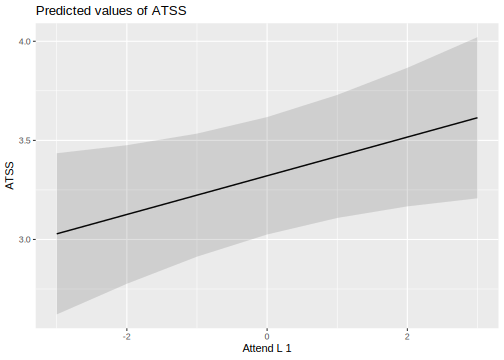
\includegraphics{ReC_Multilevel_files/figure-latex/unnamed-chunk-7-1.pdf}
MLM is a little different than other statistics in that our evaluation of the statistical assumptions continues through the evaluative process. The diagnostic plots (type = ``diag'') provide a check of the model assumptions. Each of the plots provides some guidance of how to interpret them to see if we have violated the assumptions. In the QQ plots, the points generally track along the lines. In the non-normality of residuals, our distribution approximates the superimposed normal curve. In the homoscedasticity plot, the points are scattered above/blow the line in a reasonably equal amounts with random spread.

\begin{Shaded}
\begin{Highlighting}[]
\NormalTok{sjPlot}\SpecialCharTok{::}\FunctionTok{plot\_model}\NormalTok{ (Mod2, }\AttributeTok{type=}\StringTok{"diag"}\NormalTok{)}
\end{Highlighting}
\end{Shaded}

\begin{verbatim}
[[1]]
\end{verbatim}

\begin{verbatim}
`geom_smooth()` using formula 'y ~ x'
\end{verbatim}

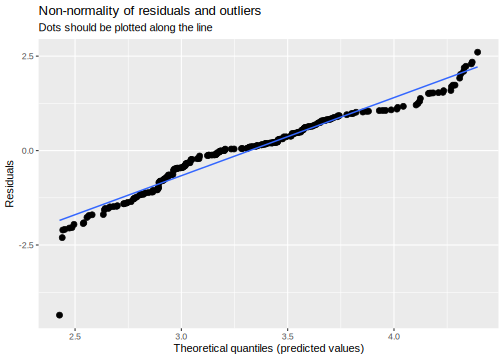
\includegraphics{ReC_Multilevel_files/figure-latex/unnamed-chunk-8-1.pdf}

\begin{verbatim}
[[2]]
[[2]]$church
\end{verbatim}

\begin{verbatim}
`geom_smooth()` using formula 'y ~ x'
\end{verbatim}

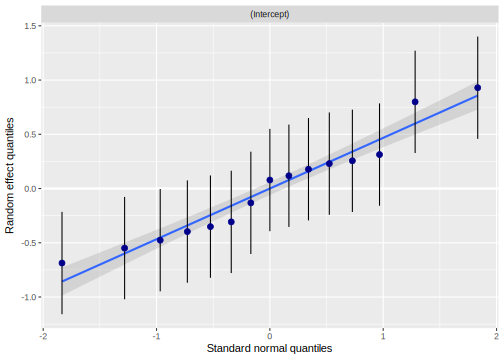
\includegraphics{ReC_Multilevel_files/figure-latex/unnamed-chunk-8-2.pdf}

\begin{verbatim}

[[3]]
\end{verbatim}

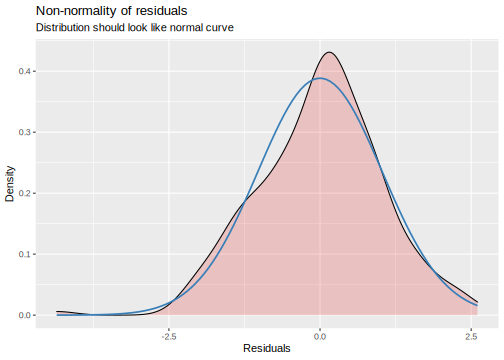
\includegraphics{ReC_Multilevel_files/figure-latex/unnamed-chunk-8-3.pdf}

\begin{verbatim}
[[4]]
\end{verbatim}

\begin{verbatim}
`geom_smooth()` using formula 'y ~ x'
\end{verbatim}

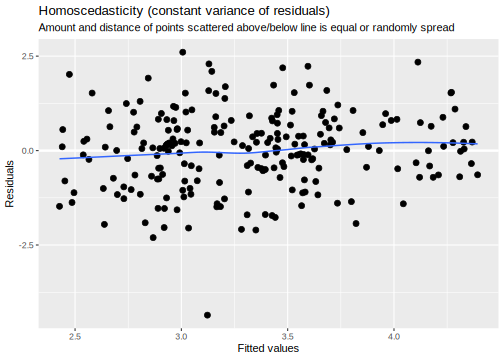
\includegraphics{ReC_Multilevel_files/figure-latex/unnamed-chunk-8-4.pdf}

With the \emph{plot\_model()} function in \emph{sjPlot}, we can plot the random effects. For this intercept-only model, we see the mean and range of the ATSS variable.

Summarizing what we learned in Mod2:

\begin{itemize}
\tightlist
\item
  An individual's church attendance (relative to others in their church) has a significant effect on homonegativity.
\item
  The addition of this L1 variable accounted for a little of the within-church variance, but there is justification for adding additional L1 variables.
\item
  There appears to be between-church variance. Thus, adding L2 variables is justified.
\item
  The L1 model is an improvement over the empty model.
\end{itemize}

Although Lefevor and colleagues \citeyearpar{lefevor_homonegativity_2020} included more L1 variables (you can choose one or more of them for practice), because the purpose of this is instructional, we will proceed by adding two, L2 variables. The first is the aggregate form of church attendance (AttendL2), the second is an exclusive L2 variable, homogeneity (proportion of Black congregants).

\hypertarget{model-3-adding-the-l2-predictors}{%
\subsubsection{Model 3: Adding the L2 predictors}\label{model-3-adding-the-l2-predictors}}

\begin{Shaded}
\begin{Highlighting}[]
\CommentTok{\# MODEL 3}
\NormalTok{Mod3 }\OtherTok{\textless{}{-}} \FunctionTok{lmer}\NormalTok{(ATSS }\SpecialCharTok{\textasciitilde{}}\NormalTok{ AttendL1 }\SpecialCharTok{+}\NormalTok{ AttendL2 }\SpecialCharTok{+}\NormalTok{ Homogeneity }\SpecialCharTok{+}\NormalTok{ (}\DecValTok{1} \SpecialCharTok{|}\NormalTok{ church), }\AttributeTok{REML=}\ConstantTok{FALSE}\NormalTok{, }\AttributeTok{data =}\NormalTok{ Lefevor2020)}
\FunctionTok{summary}\NormalTok{(Mod3)}
\end{Highlighting}
\end{Shaded}

\begin{verbatim}
Linear mixed model fit by maximum likelihood . t-tests use Satterthwaite's
  method [lmerModLmerTest]
Formula: ATSS ~ AttendL1 + AttendL2 + Homogeneity + (1 | church)
   Data: Lefevor2020

     AIC      BIC   logLik deviance df.resid 
   687.5    708.0   -337.8    675.5      219 

Scaled residuals: 
    Min      1Q  Median      3Q     Max 
-4.4350 -0.6238  0.0782  0.6362  2.2297 

Random effects:
 Groups   Name        Variance Std.Dev.
 church   (Intercept) 0.1141   0.3378  
 Residual             1.1075   1.0524  
Number of obs: 225, groups:  church, 15

Fixed effects:
             Estimate Std. Error        df t value Pr(>|t|)   
(Intercept)   4.85555    2.70843  15.00000   1.793  0.09320 . 
AttendL1      0.09763    0.04738 210.00000   2.061  0.04056 * 
AttendL2      0.01658    0.37518  15.00000   0.044  0.96533   
Homogeneity  -1.59347    0.47613  15.00000  -3.347  0.00441 **
---
Signif. codes:  0 '***' 0.001 '**' 0.01 '*' 0.05 '.' 0.1 ' ' 1

Correlation of Fixed Effects:
            (Intr) AttnL1 AttnL2
AttendL1     0.000              
AttendL2    -0.984  0.000       
Homogeneity  0.147  0.000 -0.317
\end{verbatim}

\begin{Shaded}
\begin{Highlighting}[]
\FunctionTok{AIC}\NormalTok{(Mod3) }\CommentTok{\# request AIC}
\end{Highlighting}
\end{Shaded}

\begin{verbatim}
[1] 687.5166
\end{verbatim}

\begin{Shaded}
\begin{Highlighting}[]
\FunctionTok{BIC}\NormalTok{(Mod3) }\CommentTok{\# request BIC}
\end{Highlighting}
\end{Shaded}

\begin{verbatim}
[1] 708.0132
\end{verbatim}

\begin{Shaded}
\begin{Highlighting}[]
\NormalTok{ModB3 }\OtherTok{\textless{}{-}} \FunctionTok{lme}\NormalTok{(ATSS }\SpecialCharTok{\textasciitilde{}}\NormalTok{  AttendL1 }\SpecialCharTok{+}\NormalTok{  AttendL2 }\SpecialCharTok{+}\NormalTok{ Homogeneity, }\AttributeTok{random =} \SpecialCharTok{\textasciitilde{}} \DecValTok{1}\SpecialCharTok{|}\NormalTok{church, }\AttributeTok{method=}\StringTok{"ML"}\NormalTok{, }\AttributeTok{na.action =}\NormalTok{ na.omit, }\AttributeTok{data =}\NormalTok{Lefevor2020)}
\FunctionTok{summary}\NormalTok{(Mod3)}
\end{Highlighting}
\end{Shaded}

\begin{verbatim}
Linear mixed model fit by maximum likelihood . t-tests use Satterthwaite's
  method [lmerModLmerTest]
Formula: ATSS ~ AttendL1 + AttendL2 + Homogeneity + (1 | church)
   Data: Lefevor2020

     AIC      BIC   logLik deviance df.resid 
   687.5    708.0   -337.8    675.5      219 

Scaled residuals: 
    Min      1Q  Median      3Q     Max 
-4.4350 -0.6238  0.0782  0.6362  2.2297 

Random effects:
 Groups   Name        Variance Std.Dev.
 church   (Intercept) 0.1141   0.3378  
 Residual             1.1075   1.0524  
Number of obs: 225, groups:  church, 15

Fixed effects:
             Estimate Std. Error        df t value Pr(>|t|)   
(Intercept)   4.85555    2.70843  15.00000   1.793  0.09320 . 
AttendL1      0.09763    0.04738 210.00000   2.061  0.04056 * 
AttendL2      0.01658    0.37518  15.00000   0.044  0.96533   
Homogeneity  -1.59347    0.47613  15.00000  -3.347  0.00441 **
---
Signif. codes:  0 '***' 0.001 '**' 0.01 '*' 0.05 '.' 0.1 ' ' 1

Correlation of Fixed Effects:
            (Intr) AttnL1 AttnL2
AttendL1     0.000              
AttendL2    -0.984  0.000       
Homogeneity  0.147  0.000 -0.317
\end{verbatim}

\begin{Shaded}
\begin{Highlighting}[]
\FunctionTok{anova}\NormalTok{(Mod3) }\CommentTok{\# request F{-}tests for fixed effects}
\end{Highlighting}
\end{Shaded}

\begin{verbatim}
Type III Analysis of Variance Table with Satterthwaite's method
             Sum Sq Mean Sq NumDF DenDF F value   Pr(>F)   
AttendL1     4.7032  4.7032     1   210  4.2466 0.040562 * 
AttendL2     0.0022  0.0022     1    15  0.0020 0.965326   
Homogeneity 12.4049 12.4049     1    15 11.2005 0.004415 **
---
Signif. codes:  0 '***' 0.001 '**' 0.01 '*' 0.05 '.' 0.1 ' ' 1
\end{verbatim}

\begin{Shaded}
\begin{Highlighting}[]
\FunctionTok{ranova}\NormalTok{(Mod3) }\CommentTok{\# request test of random effects}
\end{Highlighting}
\end{Shaded}

\begin{verbatim}
ANOVA-like table for random-effects: Single term deletions

Model:
ATSS ~ AttendL1 + AttendL2 + Homogeneity + (1 | church)
             npar  logLik    AIC    LRT Df Pr(>Chisq)   
<none>          6 -337.76 687.52                        
(1 | church)    5 -341.78 693.57 8.0497  1   0.004551 **
---
Signif. codes:  0 '***' 0.001 '**' 0.01 '*' 0.05 '.' 0.1 ' ' 1
\end{verbatim}

\begin{Shaded}
\begin{Highlighting}[]
\FunctionTok{confint}\NormalTok{(Mod3) }\CommentTok{\# request test of random effects (variance displayed as SD)}
\end{Highlighting}
\end{Shaded}

\begin{verbatim}
Computing profile confidence intervals ...
\end{verbatim}

\begin{verbatim}
                   2.5 %     97.5 %
.sig01       0.153249528  0.5914827
.sigma       0.959236807  1.1616599
(Intercept) -0.811596834 10.5226949
AttendL1     0.004347107  0.1909123
AttendL2    -0.768446894  0.8016149
Homogeneity -2.589725095 -0.5972141
\end{verbatim}

\begin{Shaded}
\begin{Highlighting}[]
\NormalTok{devM3 }\OtherTok{\textless{}{-}} \FunctionTok{anova}\NormalTok{(Mod1, Mod2, Mod3) }

\FunctionTok{tab\_model}\NormalTok{(Mod1, Mod2, Mod3, }\AttributeTok{p.style =} \StringTok{"numeric"}\NormalTok{, }\AttributeTok{show.ci =} \ConstantTok{FALSE}\NormalTok{, }\AttributeTok{show.df =} \ConstantTok{FALSE}\NormalTok{, }\AttributeTok{show.re.var =} \ConstantTok{TRUE}\NormalTok{, }\AttributeTok{show.aic =} \ConstantTok{TRUE}\NormalTok{, }\AttributeTok{show.dev =} \ConstantTok{TRUE}\NormalTok{, }\AttributeTok{use.viewer =} \ConstantTok{TRUE}\NormalTok{, }\AttributeTok{dv.labels =} \FunctionTok{c}\NormalTok{(}\StringTok{"Mod1"}\NormalTok{, }\StringTok{"Mod2"}\NormalTok{, }\StringTok{"Mod3"}\NormalTok{))}
\end{Highlighting}
\end{Shaded}

~

Mod1

Mod2

Mod3

Predictors

Estimates

p

Estimates

p

Estimates

p

(Intercept)

3.32

\textless0.001

3.32

\textless0.001

4.86

0.073

AttendL1

0.10

0.039

0.10

0.039

AttendL2

0.02

0.965

Homogeneity

-1.59

0.001

Random Effects

σ2

1.13

1.11

1.11

τ00

0.27 church

0.27 church

0.11 church

ICC

0.19

0.20

0.09

N

15 church

15 church

15 church

Observations

225

225

225

Marginal R2 / Conditional R2

0.000 / 0.191

0.015 / 0.207

0.126 / 0.208

Deviance

688.730

684.526

675.517

AIC

694.730

692.526

687.517

\begin{Shaded}
\begin{Highlighting}[]
\CommentTok{\#can swap this statement with the "file = "TabMod\_Table"" to get Viewer output or the outfile that you can open in Word}
\CommentTok{\#file = "TabMod\_Table.doc"}
\end{Highlighting}
\end{Shaded}

Again, looking at the Viewer we can look at the three models side by side. We observe:

\begin{itemize}
\tightlist
\item
  The intercept changes values. The value of 4.86 is the mean when AttendL1 is average for its church (recall we mean centered it so that 0.0 is the church mean), AttendL2 is the mean across churches, and racial homogeneity is 0.00.\\
\item
  There is now a row that includes our two L2 predictors: AttendL2 (aggregate of AttendL1) and Homogeneity (racial homogeneity of each church).
\item
  AttendL1 remains significant (with the values of the \(B\) and \(p\) remaining the same; but the L2 aggregate does not add in a significant manner
\item
  AttendL2 is not a significant predictor.
\item
  Homogeneity is a significant predictor. For every 1 unit increase in racial homogeneity, ATSS values decrease (i.e., there is a decrease in homonegativity).
\item
  \(\sigma^{2}\) is an indicator of within-church variance. This value declined from Mod1 to Mod2 (1.13 to 1.11), but has held constant. Given that we added an L2 (between-church) variables, this is sensible. Because there is within-church variance remaining, we might consider adding another L1 variable.
\item
  \(\tau _{00}\) is an indicator of between-group variance. This value dropped from 0.27 to .11. Given that AttendL2 and Homogeneity were between-church variables, this is sensible. There is some between church variance remaining.
\item
  The ICC dropped, indicating that 9\% of the remaining (unaccounted for) variance is between groups.
\item
  \textbf{Marginal} \(R^2\), the variance attributed to the fixed effects (in this case, the AttendL1 variable) increased to 13\%.
\item
  Similarly, \textbf{Conditional} \(R^2\), the variance attributed to both the fixed and random effects increased to 21\%.
\item
  AIC values that are lower indicate a better fitting model. There is no formal way to compare these values, but we see that the Mod3 value is lower.
\item
  We can call up the object we created to formally compare the deviance statistics.
\end{itemize}

\begin{Shaded}
\begin{Highlighting}[]
\NormalTok{devM3}
\end{Highlighting}
\end{Shaded}

\begin{verbatim}
Data: Lefevor2020
Models:
Mod1: ATSS ~ 1 + (1 | church)
Mod2: ATSS ~ AttendL1 + (1 | church)
Mod3: ATSS ~ AttendL1 + AttendL2 + Homogeneity + (1 | church)
     npar    AIC    BIC  logLik deviance  Chisq Df Pr(>Chisq)  
Mod1    3 694.73 704.98 -344.37   688.73                       
Mod2    4 692.53 706.19 -342.26   684.53 4.2042  1    0.04032 *
Mod3    6 687.52 708.01 -337.76   675.52 9.0093  2    0.01106 *
---
Signif. codes:  0 '***' 0.001 '**' 0.01 '*' 0.05 '.' 0.1 ' ' 1
\end{verbatim}

This repeats the comparison of Mod2 to Mod1 (it was significant). The comparison of Mod3 to Mod2 suggests even more statistically significant improvement. Specifically, \(\chi ^{2}(2) = 9.009, p = .011\)

Let's look at plots. With three predictors, we can examine each of their relations with the dependent variable. Of course they are consistent with the fixed effects:

\begin{itemize}
\tightlist
\item
  as individual church attendance (relative to others in their church) increases, homonegativity increases,
\item
  overall church attendance has no apparent effect on homonegativity, and
\item
  as racial homogeneity increases, homonegativity decreases.
\end{itemize}

\begin{Shaded}
\begin{Highlighting}[]
\NormalTok{sjPlot}\SpecialCharTok{::}\FunctionTok{plot\_model}\NormalTok{ (Mod3, }\AttributeTok{type=}\StringTok{"pred"}\NormalTok{)}
\end{Highlighting}
\end{Shaded}

\begin{verbatim}
$AttendL1
\end{verbatim}

\includegraphics{ReC_Multilevel_files/figure-latex/unnamed-chunk-9-1.pdf}

\begin{verbatim}
$AttendL2
\end{verbatim}

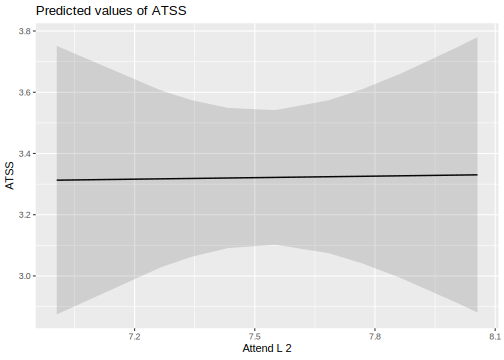
\includegraphics{ReC_Multilevel_files/figure-latex/unnamed-chunk-9-2.pdf}

\begin{verbatim}
$Homogeneity
\end{verbatim}

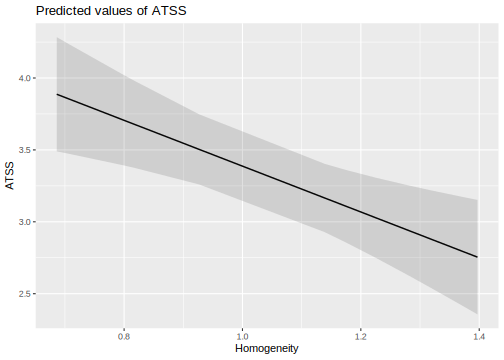
\includegraphics{ReC_Multilevel_files/figure-latex/unnamed-chunk-9-3.pdf}

Because the next phase of model building will include cross-level interactions, let's display this mode by examining the relationship between individual attendance and homonegativity, chunked into clusters that let us also examine the influene of church-level attendance and racial homogeneity. This is not a formal test of an interaction; however, I don't sense that there will be interacting effects.

\begin{Shaded}
\begin{Highlighting}[]
\NormalTok{sjPlot}\SpecialCharTok{::}\FunctionTok{plot\_model}\NormalTok{ (Mod3, }\AttributeTok{type=}\StringTok{"pred"}\NormalTok{,}\AttributeTok{terms=}\FunctionTok{c}\NormalTok{(}\StringTok{"AttendL1"}\NormalTok{, }\StringTok{"Homogeneity"}\NormalTok{, }\StringTok{"AttendL2"}\NormalTok{))}
\end{Highlighting}
\end{Shaded}

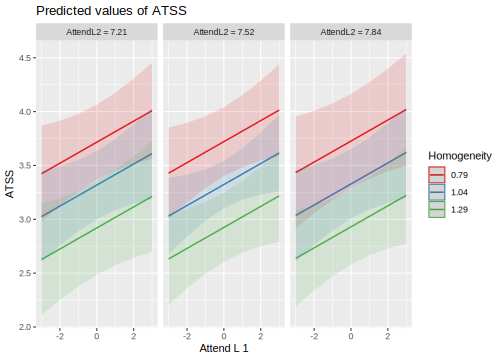
\includegraphics{ReC_Multilevel_files/figure-latex/unnamed-chunk-10-1.pdf}

Our diagnostic plots continue to support our modeling. In the QQ plots, the points generally track along the lines. In the non-normality of residuals, our distribution approximates the superimposed normal curve. In the homoscedasticity plot, the points are scattered above/blow the line in a reasonably equal amounts with random spread.

\begin{Shaded}
\begin{Highlighting}[]
\NormalTok{sjPlot}\SpecialCharTok{::}\FunctionTok{plot\_model}\NormalTok{ (Mod3, }\AttributeTok{type=}\StringTok{"diag"}\NormalTok{)}
\end{Highlighting}
\end{Shaded}

\begin{verbatim}
[[1]]
\end{verbatim}

\begin{verbatim}
`geom_smooth()` using formula 'y ~ x'
\end{verbatim}

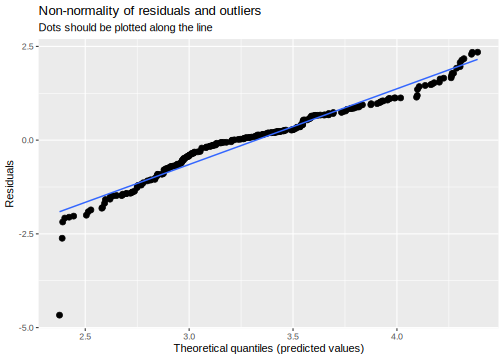
\includegraphics{ReC_Multilevel_files/figure-latex/diagnostic plots for Mod3-1.pdf}

\begin{verbatim}
[[2]]
[[2]]$church
\end{verbatim}

\begin{verbatim}
`geom_smooth()` using formula 'y ~ x'
\end{verbatim}

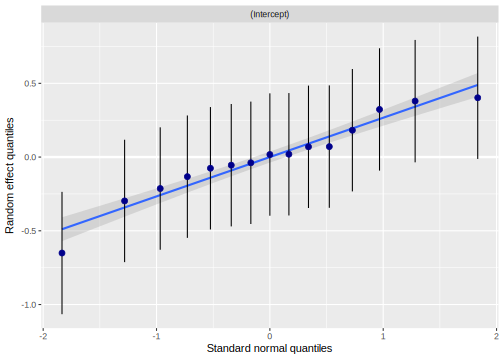
\includegraphics{ReC_Multilevel_files/figure-latex/diagnostic plots for Mod3-2.pdf}

\begin{verbatim}

[[3]]
\end{verbatim}

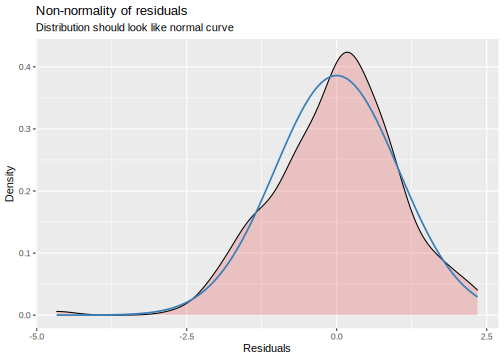
\includegraphics{ReC_Multilevel_files/figure-latex/diagnostic plots for Mod3-3.pdf}

\begin{verbatim}
[[4]]
\end{verbatim}

\begin{verbatim}
`geom_smooth()` using formula 'y ~ x'
\end{verbatim}

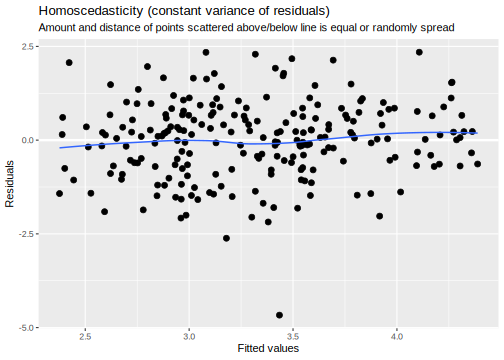
\includegraphics{ReC_Multilevel_files/figure-latex/diagnostic plots for Mod3-4.pdf}

Lefevor and colleagues \citep{lefevor_homonegativity_2020} had intended to include interaction terms. However, because only one predictor was significant at each of the individual and congregational levels, their final model did not include interaction effects. I am guessing they tried it and trimmed it out.

We add the interaction term by placing an asterisk between the two variables. There is no need (also no harm in) to enter them separately.

\hypertarget{model-4-adding-a-cross-level-interaction-term}{%
\subsubsection{Model 4: Adding a cross-level interaction term}\label{model-4-adding-a-cross-level-interaction-term}}

In multilevel modeling, we have the opportunity to cross the levels (individual, group) when we specify interactions. In this model, we include an interaction between individual attendance and racial homogeneity of the church.

\begin{Shaded}
\begin{Highlighting}[]
\CommentTok{\# MODEL 4}
\NormalTok{Mod4 }\OtherTok{\textless{}{-}} \FunctionTok{lmer}\NormalTok{(ATSS }\SpecialCharTok{\textasciitilde{}}\NormalTok{ AttendL2 }\SpecialCharTok{+}\NormalTok{ AttendL1}\SpecialCharTok{*}\NormalTok{Homogeneity }\SpecialCharTok{+}\NormalTok{(}\DecValTok{1} \SpecialCharTok{|}\NormalTok{ church), }\AttributeTok{REML=}\ConstantTok{FALSE}\NormalTok{, }\AttributeTok{data =}\NormalTok{ Lefevor2020)}
\FunctionTok{summary}\NormalTok{(Mod4)}
\end{Highlighting}
\end{Shaded}

\begin{verbatim}
Linear mixed model fit by maximum likelihood . t-tests use Satterthwaite's
  method [lmerModLmerTest]
Formula: ATSS ~ AttendL2 + AttendL1 * Homogeneity + (1 | church)
   Data: Lefevor2020

     AIC      BIC   logLik deviance df.resid 
   689.5    713.4   -337.7    675.5      218 

Scaled residuals: 
    Min      1Q  Median      3Q     Max 
-4.4652 -0.6250  0.0838  0.6268  2.2495 

Random effects:
 Groups   Name        Variance Std.Dev.
 church   (Intercept) 0.1141   0.3378  
 Residual             1.1073   1.0523  
Number of obs: 225, groups:  church, 15

Fixed effects:
                      Estimate Std. Error        df t value Pr(>|t|)   
(Intercept)            4.85555    2.70843  15.00000   1.793  0.09320 . 
AttendL2               0.01658    0.37518  15.00000   0.044  0.96533   
AttendL1               0.14098    0.21674 210.00000   0.650  0.51612   
Homogeneity           -1.59347    0.47613  15.00000  -3.347  0.00441 **
AttendL1:Homogeneity  -0.04061    0.19816 210.00000  -0.205  0.83782   
---
Signif. codes:  0 '***' 0.001 '**' 0.01 '*' 0.05 '.' 0.1 ' ' 1

Correlation of Fixed Effects:
            (Intr) AttnL2 AttnL1 Hmgnty
AttendL2    -0.984                     
AttendL1     0.000  0.000              
Homogeneity  0.147 -0.317  0.000       
AttndL1:Hmg  0.000  0.000 -0.976  0.000
\end{verbatim}

\begin{Shaded}
\begin{Highlighting}[]
\FunctionTok{AIC}\NormalTok{(Mod4) }\CommentTok{\# request AIC}
\end{Highlighting}
\end{Shaded}

\begin{verbatim}
[1] 689.4746
\end{verbatim}

\begin{Shaded}
\begin{Highlighting}[]
\FunctionTok{BIC}\NormalTok{(Mod4) }\CommentTok{\# request BIC}
\end{Highlighting}
\end{Shaded}

\begin{verbatim}
[1] 713.3873
\end{verbatim}

\begin{Shaded}
\begin{Highlighting}[]
\NormalTok{ModB3 }\OtherTok{\textless{}{-}} \FunctionTok{lme}\NormalTok{(ATSS }\SpecialCharTok{\textasciitilde{}}\NormalTok{  AttendL2 }\SpecialCharTok{+}\NormalTok{ AttendL1}\SpecialCharTok{*}\NormalTok{Homogeneity, }\AttributeTok{random =} \SpecialCharTok{\textasciitilde{}} \DecValTok{1}\SpecialCharTok{|}\NormalTok{church, }\AttributeTok{method=}\StringTok{"ML"}\NormalTok{, }\AttributeTok{na.action =}\NormalTok{ na.omit, }\AttributeTok{data =}\NormalTok{Lefevor2020)}
\FunctionTok{summary}\NormalTok{(Mod4)}
\end{Highlighting}
\end{Shaded}

\begin{verbatim}
Linear mixed model fit by maximum likelihood . t-tests use Satterthwaite's
  method [lmerModLmerTest]
Formula: ATSS ~ AttendL2 + AttendL1 * Homogeneity + (1 | church)
   Data: Lefevor2020

     AIC      BIC   logLik deviance df.resid 
   689.5    713.4   -337.7    675.5      218 

Scaled residuals: 
    Min      1Q  Median      3Q     Max 
-4.4652 -0.6250  0.0838  0.6268  2.2495 

Random effects:
 Groups   Name        Variance Std.Dev.
 church   (Intercept) 0.1141   0.3378  
 Residual             1.1073   1.0523  
Number of obs: 225, groups:  church, 15

Fixed effects:
                      Estimate Std. Error        df t value Pr(>|t|)   
(Intercept)            4.85555    2.70843  15.00000   1.793  0.09320 . 
AttendL2               0.01658    0.37518  15.00000   0.044  0.96533   
AttendL1               0.14098    0.21674 210.00000   0.650  0.51612   
Homogeneity           -1.59347    0.47613  15.00000  -3.347  0.00441 **
AttendL1:Homogeneity  -0.04061    0.19816 210.00000  -0.205  0.83782   
---
Signif. codes:  0 '***' 0.001 '**' 0.01 '*' 0.05 '.' 0.1 ' ' 1

Correlation of Fixed Effects:
            (Intr) AttnL2 AttnL1 Hmgnty
AttendL2    -0.984                     
AttendL1     0.000  0.000              
Homogeneity  0.147 -0.317  0.000       
AttndL1:Hmg  0.000  0.000 -0.976  0.000
\end{verbatim}

\begin{Shaded}
\begin{Highlighting}[]
\FunctionTok{anova}\NormalTok{(Mod4) }\CommentTok{\# request F{-}tests for fixed effects}
\end{Highlighting}
\end{Shaded}

\begin{verbatim}
Type III Analysis of Variance Table with Satterthwaite's method
                      Sum Sq Mean Sq NumDF DenDF F value   Pr(>F)   
AttendL2              0.0022  0.0022     1    15  0.0020 0.965326   
AttendL1              0.4685  0.4685     1   210  0.4231 0.516125   
Homogeneity          12.4024 12.4024     1    15 11.2005 0.004415 **
AttendL1:Homogeneity  0.0465  0.0465     1   210  0.0420 0.837816   
---
Signif. codes:  0 '***' 0.001 '**' 0.01 '*' 0.05 '.' 0.1 ' ' 1
\end{verbatim}

\begin{Shaded}
\begin{Highlighting}[]
\FunctionTok{ranova}\NormalTok{(Mod4) }\CommentTok{\# request test of random effects}
\end{Highlighting}
\end{Shaded}

\begin{verbatim}
ANOVA-like table for random-effects: Single term deletions

Model:
ATSS ~ AttendL2 + AttendL1 + Homogeneity + (1 | church) + AttendL1:Homogeneity
             npar  logLik    AIC    LRT Df Pr(>Chisq)   
<none>          7 -337.74 689.47                        
(1 | church)    6 -341.76 695.53 8.0536  1   0.004541 **
---
Signif. codes:  0 '***' 0.001 '**' 0.01 '*' 0.05 '.' 0.1 ' ' 1
\end{verbatim}

\begin{Shaded}
\begin{Highlighting}[]
\FunctionTok{confint}\NormalTok{(Mod4) }\CommentTok{\# request test of random effects (variance displayed as SD)}
\end{Highlighting}
\end{Shaded}

\begin{verbatim}
Computing profile confidence intervals ...
\end{verbatim}

\begin{verbatim}
                          2.5 %     97.5 %
.sig01                0.1533133  0.5914950
.sigma                0.9591409  1.1615437
(Intercept)          -0.8115834 10.5226817
AttendL2             -0.7684450  0.8016131
AttendL1             -0.2857791  0.5677291
Homogeneity          -2.5897227 -0.5972164
AttendL1:Homogeneity -0.4307735  0.3495523
\end{verbatim}

\begin{Shaded}
\begin{Highlighting}[]
\NormalTok{devM4 }\OtherTok{\textless{}{-}} \FunctionTok{anova}\NormalTok{(Mod1, Mod2, Mod3, Mod4) }
\FunctionTok{tab\_model}\NormalTok{(Mod1, Mod2, Mod3, Mod4, }\AttributeTok{p.style =} \StringTok{"numeric"}\NormalTok{, }\AttributeTok{show.ci =} \ConstantTok{FALSE}\NormalTok{, }\AttributeTok{show.df =} \ConstantTok{FALSE}\NormalTok{, }\AttributeTok{show.re.var =} \ConstantTok{TRUE}\NormalTok{, }\AttributeTok{show.aic =} \ConstantTok{TRUE}\NormalTok{, }\AttributeTok{show.dev =} \ConstantTok{TRUE}\NormalTok{, }\AttributeTok{use.viewer =} \ConstantTok{TRUE}\NormalTok{, }\AttributeTok{dv.labels =} \FunctionTok{c}\NormalTok{(}\StringTok{"Mod1"}\NormalTok{, }\StringTok{"Mod2"}\NormalTok{, }\StringTok{"Mod3"}\NormalTok{, }\StringTok{"Mod4"}\NormalTok{))}
\end{Highlighting}
\end{Shaded}

~

Mod1

Mod2

Mod3

Mod4

Predictors

Estimates

p

Estimates

p

Estimates

p

Estimates

p

(Intercept)

3.32

\textless0.001

3.32

\textless0.001

4.86

0.073

4.86

0.073

AttendL1

0.10

0.039

0.10

0.039

0.14

0.515

AttendL2

0.02

0.965

0.02

0.965

Homogeneity

-1.59

0.001

-1.59

0.001

AttendL1 * Homogeneity

-0.04

0.838

Random Effects

σ2

1.13

1.11

1.11

1.11

τ00

0.27 church

0.27 church

0.11 church

0.11 church

ICC

0.19

0.20

0.09

0.09

N

15 church

15 church

15 church

15 church

Observations

225

225

225

225

Marginal R2 / Conditional R2

0.000 / 0.191

0.015 / 0.207

0.126 / 0.208

0.126 / 0.208

Deviance

688.730

684.526

675.517

675.475

AIC

694.730

692.526

687.517

689.475

\begin{Shaded}
\begin{Highlighting}[]
\CommentTok{\#can swap this statement with the "file = "TabMod\_Table"" to get Viewer output or the outfile that you can open in Word}
\CommentTok{\#file = "TabMod\_Table.doc"}
\end{Highlighting}
\end{Shaded}

Again, looking at the Viewer we can look at the four models side by side. We observe:

\begin{itemize}
\tightlist
\item
  Although the B weight increases from 0.10 to 0.14, we lose the significance associated with AttendL1.
\item
  The AttendL1*Homogeneity interaction effect is non-significant.
\item
  There are no changes in our random effects (e.g., \(\sigma^{2}\) and \(\tau _{00}\), nor the \textbf{Marginal} and \textbf{Conditional} \(R^2\)
\item
  The AIC value increases -- meaning that Mod4 is worse than Mod3.
\item
  Examining the formal comparison of Mod4 to Mod3 suggests no statistically significant difference (\(\chi_{2}(1) = 0.838\)).
\end{itemize}

\begin{Shaded}
\begin{Highlighting}[]
\NormalTok{devM4}
\end{Highlighting}
\end{Shaded}

\begin{verbatim}
Data: Lefevor2020
Models:
Mod1: ATSS ~ 1 + (1 | church)
Mod2: ATSS ~ AttendL1 + (1 | church)
Mod3: ATSS ~ AttendL1 + AttendL2 + Homogeneity + (1 | church)
Mod4: ATSS ~ AttendL2 + AttendL1 * Homogeneity + (1 | church)
     npar    AIC    BIC  logLik deviance  Chisq Df Pr(>Chisq)  
Mod1    3 694.73 704.98 -344.37   688.73                       
Mod2    4 692.53 706.19 -342.26   684.53 4.2042  1    0.04032 *
Mod3    6 687.52 708.01 -337.76   675.52 9.0093  2    0.01106 *
Mod4    7 689.47 713.39 -337.74   675.47 0.0420  1    0.83763  
---
Signif. codes:  0 '***' 0.001 '**' 0.01 '*' 0.05 '.' 0.1 ' ' 1
\end{verbatim}

Not surprisingly, our resultant models are consistent with the ``peek'' we took at an interaction term after Mod3.

\begin{Shaded}
\begin{Highlighting}[]
\NormalTok{sjPlot}\SpecialCharTok{::}\FunctionTok{plot\_model}\NormalTok{ (Mod4, }\AttributeTok{type=}\StringTok{"pred"}\NormalTok{,}\AttributeTok{terms=}\FunctionTok{c}\NormalTok{(}\StringTok{"AttendL1"}\NormalTok{, }\StringTok{"Homogeneity"}\NormalTok{, }\StringTok{"AttendL2"}\NormalTok{), }\AttributeTok{mdrt.values =} \StringTok{"meansd"}\NormalTok{)}
\end{Highlighting}
\end{Shaded}

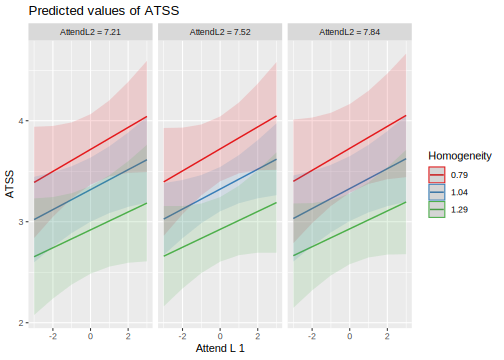
\includegraphics{ReC_Multilevel_files/figure-latex/unnamed-chunk-12-1.pdf}
Another way to view this is to request the ``int'' (interaction) model type.

\begin{Shaded}
\begin{Highlighting}[]
\NormalTok{sjPlot}\SpecialCharTok{::}\FunctionTok{plot\_model}\NormalTok{ (Mod4, }\AttributeTok{type=}\StringTok{"int"}\NormalTok{, }\AttributeTok{terms=}\FunctionTok{c}\NormalTok{(}\StringTok{"AttendL1"}\NormalTok{, }\StringTok{"AttendL2"}\NormalTok{, }\StringTok{"Homogeneity"}\NormalTok{), }\AttributeTok{mdrt.values =} \StringTok{"meansd"}\NormalTok{)}
\end{Highlighting}
\end{Shaded}

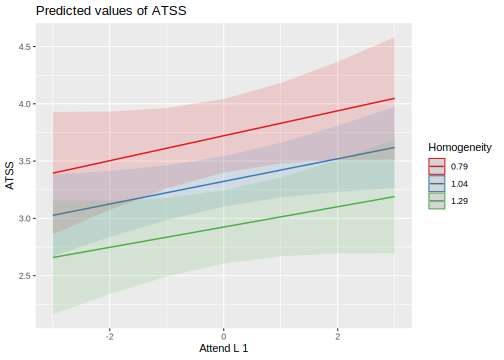
\includegraphics{ReC_Multilevel_files/figure-latex/unnamed-chunk-13-1.pdf}
Even though the addition of the interaction term did not improve our model, it does not look like it harmed it. These diagnostics remain consistent with those we saw before.

\begin{Shaded}
\begin{Highlighting}[]
\NormalTok{sjPlot}\SpecialCharTok{::}\FunctionTok{plot\_model}\NormalTok{ (Mod4, }\AttributeTok{type=}\StringTok{"diag"}\NormalTok{)}
\end{Highlighting}
\end{Shaded}

\begin{verbatim}
[[1]]
\end{verbatim}

\begin{verbatim}
`geom_smooth()` using formula 'y ~ x'
\end{verbatim}

\includegraphics{ReC_Multilevel_files/figure-latex/unnamed-chunk-14-1.pdf}

\begin{verbatim}
[[2]]
[[2]]$church
\end{verbatim}

\begin{verbatim}
`geom_smooth()` using formula 'y ~ x'
\end{verbatim}

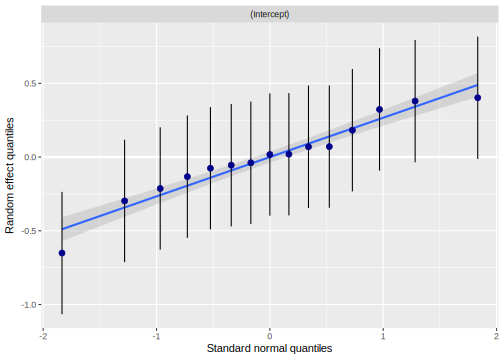
\includegraphics{ReC_Multilevel_files/figure-latex/unnamed-chunk-14-2.pdf}

\begin{verbatim}

[[3]]
\end{verbatim}

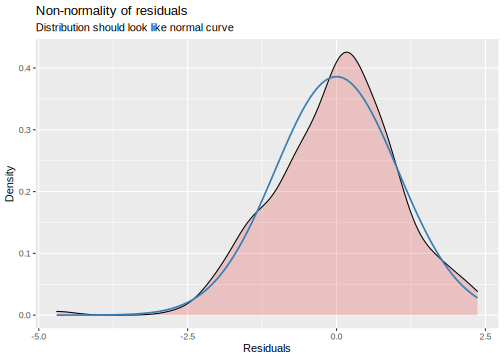
\includegraphics{ReC_Multilevel_files/figure-latex/unnamed-chunk-14-3.pdf}

\begin{verbatim}
[[4]]
\end{verbatim}

\begin{verbatim}
`geom_smooth()` using formula 'y ~ x'
\end{verbatim}

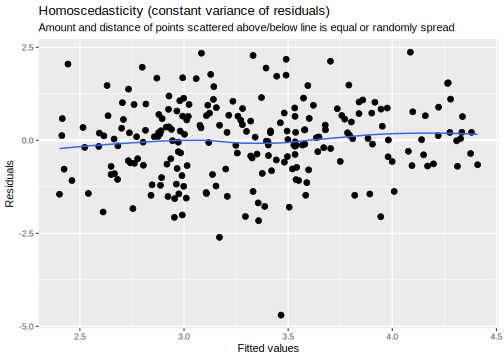
\includegraphics{ReC_Multilevel_files/figure-latex/unnamed-chunk-14-4.pdf}

\hypertarget{final-model}{%
\subsection{Final Model}\label{final-model}}

Our analysis is consistent with Lefevor and colleagues' decision to stop after Mod3. Therefore I will ``trim'' the interaction term out.

\begin{Shaded}
\begin{Highlighting}[]
\CommentTok{\# MODEL 3}
\NormalTok{Mod3 }\OtherTok{\textless{}{-}} \FunctionTok{lmer}\NormalTok{(ATSS }\SpecialCharTok{\textasciitilde{}}\NormalTok{ AttendL1 }\SpecialCharTok{+}\NormalTok{ AttendL2 }\SpecialCharTok{+}\NormalTok{ Homogeneity }\SpecialCharTok{+}\NormalTok{ (}\DecValTok{1} \SpecialCharTok{|}\NormalTok{ church), }\AttributeTok{REML=}\ConstantTok{FALSE}\NormalTok{, }\AttributeTok{data =}\NormalTok{ Lefevor2020)}
\FunctionTok{summary}\NormalTok{(Mod3)}
\end{Highlighting}
\end{Shaded}

\begin{verbatim}
Linear mixed model fit by maximum likelihood . t-tests use Satterthwaite's
  method [lmerModLmerTest]
Formula: ATSS ~ AttendL1 + AttendL2 + Homogeneity + (1 | church)
   Data: Lefevor2020

     AIC      BIC   logLik deviance df.resid 
   687.5    708.0   -337.8    675.5      219 

Scaled residuals: 
    Min      1Q  Median      3Q     Max 
-4.4350 -0.6238  0.0782  0.6362  2.2297 

Random effects:
 Groups   Name        Variance Std.Dev.
 church   (Intercept) 0.1141   0.3378  
 Residual             1.1075   1.0524  
Number of obs: 225, groups:  church, 15

Fixed effects:
             Estimate Std. Error        df t value Pr(>|t|)   
(Intercept)   4.85555    2.70843  15.00000   1.793  0.09320 . 
AttendL1      0.09763    0.04738 210.00000   2.061  0.04056 * 
AttendL2      0.01658    0.37518  15.00000   0.044  0.96533   
Homogeneity  -1.59347    0.47613  15.00000  -3.347  0.00441 **
---
Signif. codes:  0 '***' 0.001 '**' 0.01 '*' 0.05 '.' 0.1 ' ' 1

Correlation of Fixed Effects:
            (Intr) AttnL1 AttnL2
AttendL1     0.000              
AttendL2    -0.984  0.000       
Homogeneity  0.147  0.000 -0.317
\end{verbatim}

\begin{Shaded}
\begin{Highlighting}[]
\CommentTok{\#AIC(Mod3) \# request AIC}
\CommentTok{\#BIC(Mod3) \# request BIC}
\CommentTok{\#ModB3 \textless{}{-} lme(ATSS \textasciitilde{}  AttendL1 +  AttendL2 + Homogeneity, random = \textasciitilde{} 1|church, method="ML", na.action = na.omit, data =Lefevor2020)}
\CommentTok{\#summary(Mod3)}
\CommentTok{\#anova(Mod3) \# request F{-}tests for fixed effects}
\CommentTok{\#ranova(Mod3) \# request test of random effects}
\CommentTok{\#confint(Mod3) \# request test of random effects (variance displayed as SD)}
\NormalTok{devM3 }\OtherTok{\textless{}{-}} \FunctionTok{anova}\NormalTok{(Mod1, Mod2, Mod3) }

\FunctionTok{tab\_model}\NormalTok{(Mod1, Mod2, Mod3, }\AttributeTok{p.style =} \StringTok{"numeric"}\NormalTok{, }\AttributeTok{show.ci =} \ConstantTok{FALSE}\NormalTok{, }\AttributeTok{show.df =} \ConstantTok{FALSE}\NormalTok{, }\AttributeTok{show.re.var =} \ConstantTok{TRUE}\NormalTok{, }\AttributeTok{show.aic =} \ConstantTok{TRUE}\NormalTok{, }\AttributeTok{show.dev =} \ConstantTok{TRUE}\NormalTok{, }\AttributeTok{use.viewer =} \ConstantTok{TRUE}\NormalTok{, }\AttributeTok{dv.labels =} \FunctionTok{c}\NormalTok{(}\StringTok{"Model 1"}\NormalTok{, }\StringTok{"Model 2"}\NormalTok{, }\StringTok{"Model 3"}\NormalTok{), }\AttributeTok{file =} \StringTok{"Lefevor\_Table.doc"}\NormalTok{)}
\end{Highlighting}
\end{Shaded}

~

Model 1

Model 2

Model 3

Predictors

Estimates

p

Estimates

p

Estimates

p

(Intercept)

3.32

\textless0.001

3.32

\textless0.001

4.86

0.073

AttendL1

0.10

0.039

0.10

0.039

AttendL2

0.02

0.965

Homogeneity

-1.59

0.001

Random Effects

σ2

1.13

1.11

1.11

τ00

0.27 church

0.27 church

0.11 church

ICC

0.19

0.20

0.09

N

15 church

15 church

15 church

Observations

225

225

225

Marginal R2 / Conditional R2

0.000 / 0.191

0.015 / 0.207

0.126 / 0.208

Deviance

688.730

684.526

675.517

AIC

694.730

692.526

687.517

\begin{Shaded}
\begin{Highlighting}[]
\CommentTok{\#can swap this statement with the "file = "TabMod\_Table"" to get Viewer output or the outfile that you can open in Word}
\CommentTok{\#file = "TabMod\_Table.doc"}
\end{Highlighting}
\end{Shaded}

\hypertarget{oh-right-the-formulae}{%
\subsection{Oh right, the Formulae}\label{oh-right-the-formulae}}

Finally, the formulae (yes, plural)

Recall the simplicity of the OLS regresion equation with a single predictor:

\[\hat{Y}_{i} = \beta_{0} + \beta_{1}X_{i} + \epsilon_{i}\]
Where:

\begin{itemize}
\tightlist
\item
  \(\hat{Y}_{i}\) (the outcome) has a subscript ``\(i\)'', indicating that it is predicted for each individual.
\item
  \(\beta_{0}\) is the population \emph{intercept}
\item
  \(\beta_{1}X_{i}\) is the population unstandardized regression \emph{slope}
\item
  \(X\) is a \emph{linear} predictor of \(Y\)
\item
  \(\epsilon_{i}\) is the random error in prediction for case \emph{i}
\end{itemize}

Importantly, the intercept and slope are both \emph{fixed} in a basic linear regression model. You can recognize that the intercept and slope are fixed because they do not include a subscript \(i\) or \(j\) (as we will see later). The lack of a subscript indicates that these parameters each only take on a single value that is meant to represent the entire population intercept or slope, respectively.

Now let's take a look at the most basic \textbf{multilevel model} and compare it to the simple linear regression model above:

\[ Y_{ij} = \beta_{0j} + \beta_{1j}X_{ij} + \epsilon_{ij} \]
Where\ldots{}

\begin{itemize}
\tightlist
\item
  \(Y_{ij}\) outcome measure for individual \emph{i} in group \emph{j}
\item
  \(X_{ij}\) is the value of the predictor for individual \emph{i} in group \emph{j}
\item
  \(\beta_{0j}\) is the intercept for group \emph{j}
\item
  \(\beta_{1j}\) is the slope for group \emph{j}
\item
  \(\epsilon_{ij}\) is the residual
\end{itemize}

Does it look familiar? The only difference in between this MLM equation and the linear regression equation is that the MLM equation contains more subscripts. As you will see, this \emph{simple} update provides us with much more information. For the purpose of defining the model, let's assume that the subscript \(j\) represents a group of individuals. In the multilevel model, \(i\) can take on any value in \((1, ..., N)\), where \(N\) is the number of individuals in the study. The subscript \(j\) may take on values in \((1, ..., J)\), where \(J\) is the number of groups in the study. In this model, recognize that each group is allowed its own unique intercept and slope. You could read the entire model as:

\emph{``The outcome value for person \(i\) in group \(j\) is equal to the intercept for group \(j\), plus the slope for group \(j\) multiplied by the x-value for person \(i\) in group \(j\), plus some error that cannot be explained by the model for person \(i\) in group \(j\).''}

The errors in \(\epsilon_{ij}\) are typically assumed to be independently and identically distributed \((iid)\) \textasciitilde{}\(N(0, \sigma^2)\).

Level 2 (macro-level) regression equations carry the group structure.

\[\beta _{0j}=\gamma _{00}+\mu _{0j}\]
\[\beta _{1j}=\gamma _{10}+\mu_{1j}\]

\(\beta _{0j}\) models the differences in the group intercepts, predicting the intercept for group \emph{j}

\begin{itemize}
\tightlist
\item
  \(\gamma _{00}\) is the population regression intercept

  \begin{itemize}
  \tightlist
  \item
    the grand mean
  \end{itemize}
\item
  \(\gamma _{00}\) assesses how much group \emph{j} differs from the grand mean

  \begin{itemize}
  \tightlist
  \item
    a measure of variance
  \end{itemize}
\end{itemize}

\(\beta _{1j}\) models the differences in group slopes

\begin{itemize}
\tightlist
\item
  \(\gamma _{10}\) is a fixed or constant population slopes
\item
  \(u_{1j}\) assesses the extent to which group \emph{j}'s slope differs from the \emph{grand slope}.
\end{itemize}

\(\mu _{0j}\) and \(\mu_{1j}\) are the residuals from trying to predict the intercepts and slopes, respectively.

So far it lwe have treated the L1 and L2 equations are treated separately. We combine them to form a single \emph{multilevel} regression equation referred to as the ``mixed model.'' This is Cohen et al.'s \citeyearpar{cohen_applied_2003} rendition. As you view it, you may wonder what happened to the B- or beta weights. There are some curious traditions in MLM. When modeling nesting in groups, some researchers use the \(\gamma\) (``g'' is for group) and when modeling nesting within people, some researchers use the \(\pi\) (``p'' is for people):

\[Y_{ij}=\gamma _{10}X_{ij}+\gamma _{00}+U_{0j}+U_{ij}X_{ij}+r_{ij}\]

\hypertarget{apa-style-writeup}{%
\subsection{APA Style Writeup}\label{apa-style-writeup}}

In this write-up, please presume that the \emph{apa.cor.table} of L1 and L2 variables and the \emph{tab\_model()} table (Mod3) we created will serve as the basis for the APA style tables. I would use one of the Mod3 predictions as the graph.

\textbf{Method/Analytic Strategy}
The nested structure of our data (congregants {[}L1{]} nested within churches {[}L2{]}), multilevel modeling was appropriate because it allows for (a) the dependent nature of the congregants within their churches and (b) varying numbers of church members within each church. We analyzed the data with the \emph{lme4} (v. 1.1-26) in R (v. 4.0.5) using full maximum likelihood. We used a compositional effect \citep{enders_centering_2007} approach to center our variables. Specifically, we used group-mean centering (centering within context) for our L1 variables. Calculating their group aggregate, we entered them back into the model as L2 predictors. This allowed each predictor to completely capture within- and between-group variance.

Model development and evaluation waas approached in a systematic and sequential manner. This exploratory approach is consistent with recommendations to pursue model generating approaches in complex models \citep{bollen_testing_1993} by first understanding the relatively simpler relations between the variables \citep[e.g.,][]{hancock_hierarchical_2010, petscher_linear_2013} and assessing the viability of more complexity based on the results. Accordingly, we began with an intercept-only model. We followed sequentially by entering L1 (Model 2), L2 (Model 3), and a cross-level interaction (Model 4). Throughout we monitored variance components and fit decisions to determine our final model.

\textbf{Results}

\textbf{Preliminary Analyses}

\begin{itemize}
\tightlist
\item
  Missing data analysis and managing missing data
\item
  Bivariate correlations, means, SDs
\item
  Address assumptions; in MLM this includes

  \begin{itemize}
  \tightlist
  \item
    linearity
  \item
    homogeneity of variance
  \item
    normal distribution of the model's residuals
  \end{itemize}
\item
  Address any apriorily known limitations and concerns
\end{itemize}

\textbf{Primary Analyses}

Table \# reports the the bivariate correlations between ATSS/homonegative attitudes and the L1 and L2 predictors. Our first model was an intercept-only, ``empty'', model with ATSS/homonegative attitudes as the dependent variable and no predictors in the model. The intraclass correlation (ICC) suggested that 19\% of the variance in homonegative attitudes was between congregations; correspondingly, 81\% was within congregations (i.e., between individuals).

We added the L1 predictor of individual church attendance in the second model. As shown in Table \#, there was a significant effect such that as individual church attendance increased, so did homonegative attitudes. We added the L2 variables of the aggregate form of church attendance and racial homogeneity in our third model. The L2 form of church attendance had a non-significant effect, however racial homogeneity was significant. Specifically, as homogeneity increased, homonegativity decreased; this relationship is illustrated in Figure \#. Our fourth model (not shown) included a cross-level interaction between individual church attendance and homogeneity. Because it was non-significant, made no changes in the variance components, and caused the AIC to increase, we trimmed it from the model. Thus, Model 3 is our final model. Further support for this model is noted by the corresponding decreases in \(\sigma^{2}\) and \(\tau _{00}\) when L1 and L2 variables were added, respectively. Additionally, marginal and conditional \(R^2\) increased and formal evaluation of the deviance statistic suggested that each addition was a statistically significant improvement.

\hypertarget{residual-and-related-questions}{%
\section{Residual and Related Questions\ldots{}}\label{residual-and-related-questions}}

..that you might have; or at least I had, but if had answered them earlier it would have disrupt the flow.

STAY TUNED

\hypertarget{practice-problems}{%
\section{Practice Problems}\label{practice-problems}}

The suggested practice problem for this chapter is to conduct a MLM that includes at least one L1 predictor, at least one L2 predictor, and a cross-level interaction.

\hypertarget{problem-1-rework-the-research-vignette-as-demonstrated-but-change-the-random-seed}{%
\subsection{Problem \#1: Rework the research vignette as demonstrated, but change the random seed}\label{problem-1-rework-the-research-vignette-as-demonstrated-but-change-the-random-seed}}

If this topic feels a bit overwhelming, simply change the random seed in the data simulation, then rework the problem. This should provide minor changes to the data (maybe in the second or third decimal point), but the results will likely be very similar.

\begin{longtable}[]{@{}
  >{\raggedright\arraybackslash}p{(\columnwidth - 4\tabcolsep) * \real{0.76}}
  >{\centering\arraybackslash}p{(\columnwidth - 4\tabcolsep) * \real{0.12}}
  >{\centering\arraybackslash}p{(\columnwidth - 4\tabcolsep) * \real{0.11}}@{}}
\toprule
Assignment Component & & \\
\midrule
\endhead
1. Assign each variable to the L1 or L2 roles & 5 & \_\_\_\_\_ \\
2. Use a compositional effects approach to centering to group-mean center the L1 variables and then ``bring back'' their aggregate as an L2 variable & 5 & \_\_\_\_\_ \\
3. Model 1: empty model & 5 & \_\_\_\_\_ \\
4. Model 2: L1 predictors & 5 & \_\_\_\_\_ \\
5. Model 3: L2 predictors & 5 & \_\_\_\_\_ \\
6. Model 4: A cross-level interaction & 5 & \_\_\_\_\_ \\
7. Create a tab\_model table with the final set of models & 5 & \_\_\_\_\_ \\
8. Create a figure to represent the result & 5 & \_\_\_\_\_ \\
9. APA Style writeup & 5 & \_\_\_\_\_ \\
10. Explanation to grader & 5 & \_\_\_\_\_ \\
\textbf{Totals} & 50 & \_\_\_\_\_ \\
\bottomrule
\end{longtable}

\hypertarget{problem-2-rework-the-research-vignette-but-swap-one-or-more-variables}{%
\subsection{Problem \#2: Rework the research vignette, but swap one or more variables}\label{problem-2-rework-the-research-vignette-but-swap-one-or-more-variables}}

The research vignette analyzes a number of variables, simultaneously. We selected only two for the example. Swap out one or more variables in the multilevel model and compare your solution to the one in the chapter (and/or oNe you mimicked in the journal article). If you wish to increase your probability of finding statistically significant effects, look for hints in Table 2 of the \citep{lefevor_homonegativity_2020} research article that sources the vignettes by selecting a variable(s) with a significant relationship with your DV.

\begin{longtable}[]{@{}
  >{\raggedright\arraybackslash}p{(\columnwidth - 4\tabcolsep) * \real{0.76}}
  >{\centering\arraybackslash}p{(\columnwidth - 4\tabcolsep) * \real{0.12}}
  >{\centering\arraybackslash}p{(\columnwidth - 4\tabcolsep) * \real{0.11}}@{}}
\toprule
Assignment Component & & \\
\midrule
\endhead
1. Assign each variable to the L1 or L2 roles & 5 & \_\_\_\_\_ \\
2. Use a compositional effects approach to centering to group-mean center the L1 variables and then ``bring back'' their aggregate as an L2 variable & 5 & \_\_\_\_\_ \\
3. Model 1: empty model & 5 & \_\_\_\_\_ \\
4. Model 2: L1 predictors & 5 & \_\_\_\_\_ \\
5. Model 3: L2 predictors & 5 & \_\_\_\_\_ \\
6. Model 4: A cross-level interaction & 5 & \_\_\_\_\_ \\
7. Create a tab\_model table with the final set of models & 5 & \_\_\_\_\_ \\
8. Create a figure to represent the result & 5 & \_\_\_\_\_ \\
9. APA Style writeup & 5 & \_\_\_\_\_ \\
10. Explanation to grader & 5 & \_\_\_\_\_ \\
\textbf{Totals} & 50 & \_\_\_\_\_ \\
\bottomrule
\end{longtable}

\hypertarget{problem-3-use-other-data-that-is-available-to-you}{%
\subsection{Problem \#3: Use other data that is available to you}\label{problem-3-use-other-data-that-is-available-to-you}}

Conduct a multilevel model with data to which you have access. This could include data you simulate on your own or from a published article.

\begin{longtable}[]{@{}
  >{\raggedright\arraybackslash}p{(\columnwidth - 4\tabcolsep) * \real{0.76}}
  >{\centering\arraybackslash}p{(\columnwidth - 4\tabcolsep) * \real{0.12}}
  >{\centering\arraybackslash}p{(\columnwidth - 4\tabcolsep) * \real{0.11}}@{}}
\toprule
Assignment Component & & \\
\midrule
\endhead
1. Assign each variable to the L1 or L2 roles & 5 & \_\_\_\_\_ \\
2. Use a compositional effects approach to centering to group-mean center the L1 variables and then ``bring back'' their aggregate as an L2 variable & 5 & \_\_\_\_\_ \\
3. Model 1: empty model & 5 & \_\_\_\_\_ \\
4. Model 2: L1 predictors & 5 & \_\_\_\_\_ \\
5. Model 3: L2 predictors & 5 & \_\_\_\_\_ \\
6. Model 4: A cross-level interaction & 5 & \_\_\_\_\_ \\
7. Create a tab\_model table with the final set of models & 5 & \_\_\_\_\_ \\
8. Create a figure to represent the result & 5 & \_\_\_\_\_ \\
9. APA Style writeup & 5 & \_\_\_\_\_ \\
10. Explanation to grader & 5 & \_\_\_\_\_ \\
\textbf{Totals} & 50 & \_\_\_\_\_ \\
\bottomrule
\end{longtable}

\hypertarget{bonus-track}{%
\section{Bonus Track:}\label{bonus-track}}

\begin{figure}
\hypertarget{id}{%
\centering
\includegraphics[width=6.45833in,height=2.19792in]{images/film-strip-1.jpg}
\caption{Image of a filmstrip}\label{id}
}
\end{figure}

\hypertarget{working-the-entire-vignette}{%
\subsection{Working the Entire Vignette}\label{working-the-entire-vignette}}

Below is the script that works the entire vignette in the Lefevor et al. \citeyearpar{lefevor_homonegativity_2020} article.

\begin{Shaded}
\begin{Highlighting}[]
\FunctionTok{library}\NormalTok{(psych)}
\NormalTok{psych}\SpecialCharTok{::}\FunctionTok{pairs.panels}\NormalTok{(Lefevor2020[}\FunctionTok{c}\NormalTok{(}\StringTok{"ATSS"}\NormalTok{, }\StringTok{"Female0"}\NormalTok{, }\StringTok{"Age"}\NormalTok{, }\StringTok{"Education"}\NormalTok{, }\StringTok{"Attendance"}\NormalTok{, }\StringTok{"Homogeneity"}\NormalTok{)], }\AttributeTok{stars =} \ConstantTok{TRUE}\NormalTok{)}
\end{Highlighting}
\end{Shaded}

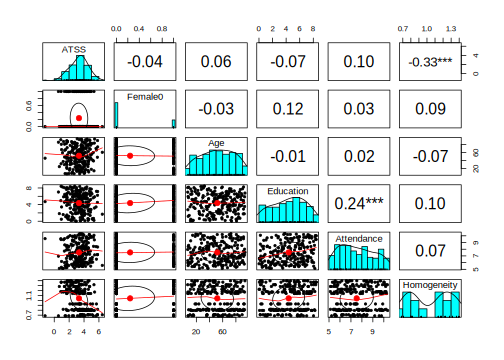
\includegraphics{ReC_Multilevel_files/figure-latex/unnamed-chunk-15-1.pdf}

\begin{Shaded}
\begin{Highlighting}[]
\NormalTok{psych}\SpecialCharTok{::}\FunctionTok{describe}\NormalTok{(Lefevor2020[}\FunctionTok{c}\NormalTok{(}\StringTok{"ATSS"}\NormalTok{, }\StringTok{"Female0"}\NormalTok{, }\StringTok{"Age"}\NormalTok{, }\StringTok{"Education"}\NormalTok{, }\StringTok{"Attendance"}\NormalTok{, }\StringTok{"Homogeneity"}\NormalTok{)])}
\end{Highlighting}
\end{Shaded}

\begin{verbatim}
            vars   n  mean    sd median trimmed   mad   min   max range  skew
ATSS           1 225  3.32  1.18   3.43    3.34  1.11 -1.23  6.45  7.69 -0.30
Female0        2 225  0.24  0.43   0.00    0.18  0.00  0.00  1.00  1.00  1.21
Age            3 225 51.78 24.62  52.80   52.15 30.05  6.91 93.76 86.85 -0.11
Education      4 225  4.37  2.35   4.62    4.42  2.76  0.01  8.44  8.43 -0.18
Attendance     5 225  7.52  1.52   7.36    7.47  1.84  5.12 10.35  5.22  0.24
Homogeneity    6 225  1.04  0.25   1.14    1.04  0.34  0.69  1.40  0.71 -0.04
            kurtosis   se
ATSS            0.27 0.08
Female0        -0.54 0.03
Age            -1.11 1.64
Education      -1.06 0.16
Attendance     -1.19 0.10
Homogeneity    -1.60 0.02
\end{verbatim}

\begin{Shaded}
\begin{Highlighting}[]
\CommentTok{\#Single level correlation matrix}
\NormalTok{apaTables}\SpecialCharTok{::}\FunctionTok{apa.cor.table}\NormalTok{(Lefevor2020[}\FunctionTok{c}\NormalTok{(}
\StringTok{"ATSS"}\NormalTok{, }\StringTok{"Female0"}\NormalTok{, }\StringTok{"Age"}\NormalTok{, }\StringTok{"Education"}\NormalTok{, }\StringTok{"Attendance"}\NormalTok{, }\StringTok{"Homogeneity"}\NormalTok{)], }\AttributeTok{show.conf.interval =} \ConstantTok{FALSE}\NormalTok{, }\AttributeTok{landscape =} \ConstantTok{TRUE}\NormalTok{, }\AttributeTok{table.number =} \DecValTok{1}\NormalTok{, }\AttributeTok{filename=}\StringTok{"CorMatrix.doc"}\NormalTok{)}
\end{Highlighting}
\end{Shaded}

\begin{verbatim}
The ability to suppress reporting of reporting confidence intervals has been deprecated in this version.
The function argument show.conf.interval will be removed in a later version.
\end{verbatim}

\begin{verbatim}

Table 1 

Means, standard deviations, and correlations with confidence intervals
 

  Variable       M     SD    1            2           3           4          
  1. ATSS        3.32  1.18                                                  
                                                                             
  2. Female0     0.24  0.43  -.04                                            
                             [-.17, .09]                                     
                                                                             
  3. Age         51.78 24.62 .06          -.03                               
                             [-.07, .19]  [-.16, .10]                        
                                                                             
  4. Education   4.37  2.35  -.07         .12         -.01                   
                             [-.20, .06]  [-.01, .25] [-.14, .12]            
                                                                             
  5. Attendance  7.52  1.52  .10          .03         .02         .24**      
                             [-.03, .23]  [-.10, .16] [-.11, .15] [.11, .36] 
                                                                             
  6. Homogeneity 1.04  0.25  -.33**       .09         -.07        .10        
                             [-.44, -.21] [-.04, .22] [-.19, .07] [-.03, .23]
                                                                             
  5          
             
             
             
             
             
             
             
             
             
             
             
             
             
             
  .07        
  [-.07, .19]
             

Note. M and SD are used to represent mean and standard deviation, respectively.
Values in square brackets indicate the 95% confidence interval.
The confidence interval is a plausible range of population correlations 
that could have caused the sample correlation (Cumming, 2014).
 * indicates p < .05. ** indicates p < .01.
 
\end{verbatim}

\begin{Shaded}
\begin{Highlighting}[]
\FunctionTok{library}\NormalTok{(robumeta)}
\NormalTok{Lefevor2020}\SpecialCharTok{$}\NormalTok{ATSSL1 }\OtherTok{\textless{}{-}} \FunctionTok{as.numeric}\NormalTok{(}\FunctionTok{group.center}\NormalTok{(Lefevor2020}\SpecialCharTok{$}\NormalTok{ATSS, Lefevor2020}\SpecialCharTok{$}\NormalTok{church))}\CommentTok{\#centered within context (group mean centering)}
\NormalTok{Lefevor2020}\SpecialCharTok{$}\NormalTok{ATSSL2 }\OtherTok{\textless{}{-}} \FunctionTok{as.numeric}\NormalTok{(}\FunctionTok{group.mean}\NormalTok{(Lefevor2020}\SpecialCharTok{$}\NormalTok{ATSS, Lefevor2020}\SpecialCharTok{$}\NormalTok{church))}\CommentTok{\#aggregated at group mean}
\NormalTok{Lefevor2020}\SpecialCharTok{$}\NormalTok{AttendL1 }\OtherTok{\textless{}{-}} \FunctionTok{as.numeric}\NormalTok{(}\FunctionTok{group.center}\NormalTok{(Lefevor2020}\SpecialCharTok{$}\NormalTok{Attendance, Lefevor2020}\SpecialCharTok{$}\NormalTok{church))}\CommentTok{\#centered within context (group mean centering)}
\NormalTok{Lefevor2020}\SpecialCharTok{$}\NormalTok{AttendL2 }\OtherTok{\textless{}{-}} \FunctionTok{as.numeric}\NormalTok{(}\FunctionTok{group.mean}\NormalTok{(Lefevor2020}\SpecialCharTok{$}\NormalTok{Attendance, Lefevor2020}\SpecialCharTok{$}\NormalTok{church))}\CommentTok{\#aggregated at group mean}
\NormalTok{Lefevor2020}\SpecialCharTok{$}\NormalTok{AgeL1 }\OtherTok{\textless{}{-}} \FunctionTok{as.numeric}\NormalTok{(}\FunctionTok{group.center}\NormalTok{(Lefevor2020}\SpecialCharTok{$}\NormalTok{Age, Lefevor2020}\SpecialCharTok{$}\NormalTok{church))}\CommentTok{\#centered within context (group mean centering)}
\NormalTok{Lefevor2020}\SpecialCharTok{$}\NormalTok{AgeL2 }\OtherTok{\textless{}{-}} \FunctionTok{as.numeric}\NormalTok{(}\FunctionTok{group.mean}\NormalTok{(Lefevor2020}\SpecialCharTok{$}\NormalTok{Age, Lefevor2020}\SpecialCharTok{$}\NormalTok{church))}\CommentTok{\#aggregated at group mean}
\NormalTok{Lefevor2020}\SpecialCharTok{$}\NormalTok{GenderL1 }\OtherTok{\textless{}{-}} \FunctionTok{as.numeric}\NormalTok{(}\FunctionTok{group.center}\NormalTok{(Lefevor2020}\SpecialCharTok{$}\NormalTok{Female0, Lefevor2020}\SpecialCharTok{$}\NormalTok{church))}\CommentTok{\#centered within context (group mean centering)}
\NormalTok{Lefevor2020}\SpecialCharTok{$}\NormalTok{GenderL2 }\OtherTok{\textless{}{-}} \FunctionTok{as.numeric}\NormalTok{(}\FunctionTok{group.mean}\NormalTok{(Lefevor2020}\SpecialCharTok{$}\NormalTok{Female0, Lefevor2020}\SpecialCharTok{$}\NormalTok{church))}\CommentTok{\#aggregated at group mean}
\NormalTok{Lefevor2020}\SpecialCharTok{$}\NormalTok{EducL1 }\OtherTok{\textless{}{-}} \FunctionTok{as.numeric}\NormalTok{(}\FunctionTok{group.center}\NormalTok{(Lefevor2020}\SpecialCharTok{$}\NormalTok{Education, Lefevor2020}\SpecialCharTok{$}\NormalTok{church))}\CommentTok{\#centered within context (group mean centering)}
\NormalTok{Lefevor2020}\SpecialCharTok{$}\NormalTok{EducL2 }\OtherTok{\textless{}{-}} \FunctionTok{as.numeric}\NormalTok{(}\FunctionTok{group.mean}\NormalTok{(Lefevor2020}\SpecialCharTok{$}\NormalTok{Education, Lefevor2020}\SpecialCharTok{$}\NormalTok{church))}\CommentTok{\#aggregated at group mean}
\end{Highlighting}
\end{Shaded}

CALCULATE L1 AND L2 ATTS

\begin{Shaded}
\begin{Highlighting}[]
\CommentTok{\#Multilevel level correlation matrix}
\NormalTok{apaTables}\SpecialCharTok{::}\FunctionTok{apa.cor.table}\NormalTok{(Lefevor2020[}\FunctionTok{c}\NormalTok{(}
\StringTok{"ATSSL1"}\NormalTok{, }\StringTok{"GenderL1"}\NormalTok{, }\StringTok{"AgeL1"}\NormalTok{, }\StringTok{"EducL1"}\NormalTok{, }\StringTok{"AttendL1"}\NormalTok{,}
\StringTok{"ATSSL2"}\NormalTok{,}\StringTok{"GenderL2"}\NormalTok{, }\StringTok{"AgeL2"}\NormalTok{, }\StringTok{"EducL2"}\NormalTok{, }\StringTok{"AttendL2"}\NormalTok{, }\StringTok{"Homogeneity"}\NormalTok{)], }\AttributeTok{show.conf.interval =} \ConstantTok{FALSE}\NormalTok{, }\AttributeTok{landscape =} \ConstantTok{TRUE}\NormalTok{, }\AttributeTok{table.number =} \DecValTok{1}\NormalTok{, }\AttributeTok{filename=}\StringTok{"ML\_CorMatrix.doc"}\NormalTok{)}
\end{Highlighting}
\end{Shaded}

\begin{verbatim}
The ability to suppress reporting of reporting confidence intervals has been deprecated in this version.
The function argument show.conf.interval will be removed in a later version.
\end{verbatim}

\begin{verbatim}

Table 1 

Means, standard deviations, and correlations with confidence intervals
 

  Variable        M     SD    1           2           3           4          
  1. ATSSL1       -0.00 1.03                                                 
                                                                             
  2. GenderL1     0.00  0.41  -.01                                           
                              [-.14, .12]                                    
                                                                             
  3. AgeL1        0.00  24.07 .05         -.04                               
                              [-.08, .18] [-.17, .09]                        
                                                                             
  4. EducL1       0.00  2.25  .01         .09         .00                    
                              [-.12, .14] [-.04, .22] [-.13, .13]            
                                                                             
  5. AttendL1     -0.00 1.48  .14*        .02         .04         .22**      
                              [.01, .27]  [-.11, .15] [-.09, .17] [.09, .34] 
                                                                             
  6. ATSSL2       3.32  0.59  .00         .00         -.00        -.00       
                              [-.13, .13] [-.13, .13] [-.13, .13] [-.13, .13]
                                                                             
  7. GenderL2     0.24  0.13  -.00        -.00        -.00        -.00       
                              [-.13, .13] [-.13, .13] [-.13, .13] [-.13, .13]
                                                                             
  8. AgeL2        51.78 5.19  .00         -.00        .00         -.00       
                              [-.13, .13] [-.13, .13] [-.13, .13] [-.13, .13]
                                                                             
  9. EducL2       4.37  0.69  -.00        .00         -.00        .00        
                              [-.13, .13] [-.13, .13] [-.13, .13] [-.13, .13]
                                                                             
  10. AttendL2    7.52  0.32  -.00        .00         -.00        .00        
                              [-.13, .13] [-.13, .13] [-.13, .13] [-.13, .13]
                                                                             
  11. Homogeneity 1.04  0.25  -.00        .00         -.00        .00        
                              [-.13, .13] [-.13, .13] [-.13, .13] [-.13, .13]
                                                                             
  5           6            7          8            9          10        
                                                                        
                                                                        
                                                                        
                                                                        
                                                                        
                                                                        
                                                                        
                                                                        
                                                                        
                                                                        
                                                                        
                                                                        
                                                                        
                                                                        
  -.00                                                                  
  [-.13, .13]                                                           
                                                                        
  -.00        -.17**                                                    
  [-.13, .13] [-.30, -.04]                                              
                                                                        
  .00         .15*         .22**                                        
  [-.13, .13] [.02, .28]   [.10, .34]                                   
                                                                        
  -.00        -.51**       .39**      -.15*                             
  [-.13, .13] [-.60, -.41] [.27, .49] [-.27, -.02]                      
                                                                        
  -.00        -.20**       .16*       -.32**       .45**                
  [-.13, .13] [-.33, -.08] [.03, .28] [-.44, -.20] [.34, .55]           
                                                                        
  -.00        -.67**       .31**      -.31**       .34**      .32**     
  [-.13, .13] [-.74, -.59] [.19, .43] [-.42, -.19] [.22, .45] [.19, .43]
                                                                        

Note. M and SD are used to represent mean and standard deviation, respectively.
Values in square brackets indicate the 95% confidence interval.
The confidence interval is a plausible range of population correlations 
that could have caused the sample correlation (Cumming, 2014).
 * indicates p < .05. ** indicates p < .01.
 
\end{verbatim}

\begin{Shaded}
\begin{Highlighting}[]
\FunctionTok{library}\NormalTok{(lme4)}

\NormalTok{ATSSm1 }\OtherTok{\textless{}{-}} \FunctionTok{lmer}\NormalTok{(ATSS }\SpecialCharTok{\textasciitilde{}}\DecValTok{1} \SpecialCharTok{+}\NormalTok{ (}\DecValTok{1} \SpecialCharTok{|}\NormalTok{ church), }\AttributeTok{REML =} \ConstantTok{FALSE}\NormalTok{, }\AttributeTok{data =}\NormalTok{ Lefevor2020)}
\FunctionTok{summary}\NormalTok{(ATSSm1)}
\end{Highlighting}
\end{Shaded}

\begin{verbatim}
Linear mixed model fit by maximum likelihood . t-tests use Satterthwaite's
  method [lmerModLmerTest]
Formula: ATSS ~ 1 + (1 | church)
   Data: Lefevor2020

     AIC      BIC   logLik deviance df.resid 
   694.7    705.0   -344.4    688.7      222 

Scaled residuals: 
    Min      1Q  Median      3Q     Max 
-3.9130 -0.6410  0.0392  0.5764  2.5252 

Random effects:
 Groups   Name        Variance Std.Dev.
 church   (Intercept) 0.2673   0.5171  
 Residual             1.1299   1.0630  
Number of obs: 225, groups:  church, 15

Fixed effects:
            Estimate Std. Error      df t value          Pr(>|t|)    
(Intercept)   3.3214     0.1511 15.0000   21.98 0.000000000000803 ***
---
Signif. codes:  0 '***' 0.001 '**' 0.01 '*' 0.05 '.' 0.1 ' ' 1
\end{verbatim}

\begin{Shaded}
\begin{Highlighting}[]
\FunctionTok{AIC}\NormalTok{(ATSSm1) }\CommentTok{\# request AIC}
\end{Highlighting}
\end{Shaded}

\begin{verbatim}
[1] 694.73
\end{verbatim}

\begin{Shaded}
\begin{Highlighting}[]
\FunctionTok{BIC}\NormalTok{(ATSSm1) }\CommentTok{\# request BIC}
\end{Highlighting}
\end{Shaded}

\begin{verbatim}
[1] 704.9783
\end{verbatim}

\begin{Shaded}
\begin{Highlighting}[]
\FunctionTok{library}\NormalTok{(nlme)}
\NormalTok{ATSSmb1 }\OtherTok{\textless{}{-}} \FunctionTok{lme}\NormalTok{(ATSS }\SpecialCharTok{\textasciitilde{}} \DecValTok{1}\NormalTok{, }\AttributeTok{random =} \SpecialCharTok{\textasciitilde{}} \DecValTok{1}\SpecialCharTok{|}\NormalTok{church, }\AttributeTok{method=}\StringTok{"ML"}\NormalTok{, }\AttributeTok{na.action =}\NormalTok{ na.omit, }\AttributeTok{data =}\NormalTok{ Lefevor2020)}
\FunctionTok{summary}\NormalTok{(ATSSmb1)}
\end{Highlighting}
\end{Shaded}

\begin{verbatim}
Linear mixed-effects model fit by maximum likelihood
  Data: Lefevor2020 
     AIC      BIC   logLik
  694.73 704.9783 -344.365

Random effects:
 Formula: ~1 | church
        (Intercept) Residual
StdDev:   0.5170587 1.062978

Fixed effects:  ATSS ~ 1 
               Value Std.Error  DF  t-value p-value
(Intercept) 3.321371 0.1514833 210 21.92566       0

Standardized Within-Group Residuals:
        Min          Q1         Med          Q3         Max 
-3.91296264 -0.64096244  0.03922427  0.57637964  2.52520439 

Number of Observations: 225
Number of Groups: 15 
\end{verbatim}

\begin{Shaded}
\begin{Highlighting}[]
\FunctionTok{anova}\NormalTok{(ATSSmb1) }\CommentTok{\# request F{-}tests for fixed effects}
\end{Highlighting}
\end{Shaded}

\begin{verbatim}
            numDF denDF  F-value p-value
(Intercept)     1   210 480.7347  <.0001
\end{verbatim}

\begin{Shaded}
\begin{Highlighting}[]
\FunctionTok{library}\NormalTok{(lmerTest)}
\FunctionTok{ranova}\NormalTok{(ATSSm1) }\CommentTok{\# request test of random effects}
\end{Highlighting}
\end{Shaded}

\begin{verbatim}
ANOVA-like table for random-effects: Single term deletions

Model:
ATSS ~ (1 | church)
             npar  logLik    AIC   LRT Df   Pr(>Chisq)    
<none>          3 -344.37 694.73                          
(1 | church)    2 -356.89 717.79 25.06  1 0.0000005558 ***
---
Signif. codes:  0 '***' 0.001 '**' 0.01 '*' 0.05 '.' 0.1 ' ' 1
\end{verbatim}

\begin{Shaded}
\begin{Highlighting}[]
\FunctionTok{confint}\NormalTok{(ATSSm1) }\CommentTok{\# request test of random effects (variance displayed as SD)}
\end{Highlighting}
\end{Shaded}

\begin{verbatim}
Computing profile confidence intervals ...
\end{verbatim}

\begin{verbatim}
                2.5 %    97.5 %
.sig01      0.3231248 0.8347723
.sigma      0.9688860 1.1733458
(Intercept) 3.0051108 3.6376320
\end{verbatim}

\begin{Shaded}
\begin{Highlighting}[]
\CommentTok{\# Extract Variances to compute R\^{}2}
\NormalTok{  var\_table }\OtherTok{=} \FunctionTok{as.data.frame}\NormalTok{(}\FunctionTok{VarCorr}\NormalTok{(ATSSm1))}
\NormalTok{  ATSSm1\_var\_tot }\OtherTok{=}\NormalTok{ var\_table[}\DecValTok{1}\NormalTok{,}\StringTok{\textquotesingle{}vcov\textquotesingle{}}\NormalTok{] }\SpecialCharTok{+}\NormalTok{ var\_table[}\DecValTok{2}\NormalTok{,}\StringTok{\textquotesingle{}vcov\textquotesingle{}}\NormalTok{] }\CommentTok{\# var\_table[1,\textquotesingle{}vcov\textquotesingle{}] = L1 var; var\_table[2,\textquotesingle{}vcov\textquotesingle{}] = L2 var;  }

\FunctionTok{library}\NormalTok{(sjPlot)}

\FunctionTok{tab\_model}\NormalTok{(ATSSm1, ATSSmb1, }\AttributeTok{p.style =} \StringTok{"stars"}\NormalTok{, }\AttributeTok{show.ci =} \ConstantTok{TRUE}\NormalTok{, }\AttributeTok{show.se =} \ConstantTok{TRUE}\NormalTok{, }\AttributeTok{show.df =} \ConstantTok{FALSE}\NormalTok{, }\AttributeTok{show.re.var =} \ConstantTok{TRUE}\NormalTok{, }\AttributeTok{show.aic =} \ConstantTok{TRUE}\NormalTok{, }\AttributeTok{show.dev =} \ConstantTok{TRUE}\NormalTok{, }\AttributeTok{use.viewer =} \ConstantTok{TRUE}\NormalTok{, }\AttributeTok{dv.labels =} \FunctionTok{c}\NormalTok{(}\StringTok{"ATSSm1"}\NormalTok{, }\StringTok{"ATSSmb1"}\NormalTok{))}
\end{Highlighting}
\end{Shaded}

~

ATSSm1

ATSSmb1

Predictors

Estimates

std. Error

CI

Estimates

std. Error

CI

(Intercept)

3.32 ***

0.15

-Inf~--~Inf

3.32 ***

0.15

-Inf~--~Inf

Random Effects

σ2

1.13

1.13

τ00

0.27 church

0.27 church

ICC

0.19

0.19

N

15 church

15 church

Observations

225

225

Marginal R2 / Conditional R2

0.000 / 0.191

0.000 / 0.191

Deviance

688.730

688.730

AIC

694.730

694.730

\begin{itemize}
\tightlist
\item
  p\textless0.05~~~** p\textless0.01~~~*** p\textless0.001
\end{itemize}

\begin{Shaded}
\begin{Highlighting}[]
\CommentTok{\#can swap this statement with the "file = "TabMod\_Table"" to get Viewer output or the outfile that you can open in Word}
\CommentTok{\#file = "TabMod\_Table.doc"}
\end{Highlighting}
\end{Shaded}

\begin{Shaded}
\begin{Highlighting}[]
\CommentTok{\# MODEL 2}
\NormalTok{ATSSm2 }\OtherTok{\textless{}{-}} \FunctionTok{lmer}\NormalTok{(ATSS }\SpecialCharTok{\textasciitilde{}}\NormalTok{ GenderL1 }\SpecialCharTok{+}\NormalTok{ AgeL1 }\SpecialCharTok{+}\NormalTok{ EducL1 }\SpecialCharTok{+}\NormalTok{ AttendL1 }\SpecialCharTok{+}\NormalTok{ (}\DecValTok{1} \SpecialCharTok{|}\NormalTok{ church), }\AttributeTok{REML=}\ConstantTok{FALSE}\NormalTok{, }\AttributeTok{data =}\NormalTok{ Lefevor2020)}
\FunctionTok{summary}\NormalTok{(ATSSm2)}
\end{Highlighting}
\end{Shaded}

\begin{verbatim}
Linear mixed model fit by maximum likelihood . t-tests use Satterthwaite's
  method [lmerModLmerTest]
Formula: ATSS ~ GenderL1 + AgeL1 + EducL1 + AttendL1 + (1 | church)
   Data: Lefevor2020

     AIC      BIC   logLik deviance df.resid 
   697.9    721.8   -341.9    683.9      218 

Scaled residuals: 
    Min      1Q  Median      3Q     Max 
-4.1484 -0.6541  0.0720  0.6251  2.4179 

Random effects:
 Groups   Name        Variance Std.Dev.
 church   (Intercept) 0.2691   0.5187  
 Residual             1.1040   1.0507  
Number of obs: 225, groups:  church, 15

Fixed effects:
              Estimate Std. Error         df t value          Pr(>|t|)    
(Intercept)   3.321371   0.151146  15.000000  21.975 0.000000000000803 ***
GenderL1     -0.032468   0.172588 210.000000  -0.188            0.8510    
AgeL1         0.002031   0.002922 210.000000   0.695            0.4878    
EducL1       -0.011469   0.032158 210.000000  -0.357            0.7217    
AttendL1      0.100379   0.048559 210.000000   2.067            0.0399 *  
---
Signif. codes:  0 '***' 0.001 '**' 0.01 '*' 0.05 '.' 0.1 ' ' 1

Correlation of Fixed Effects:
         (Intr) GndrL1 AgeL1  EducL1
GenderL1  0.000                     
AgeL1     0.000  0.044              
EducL1    0.000 -0.091  0.002       
AttendL1  0.000 -0.003 -0.041 -0.222
\end{verbatim}

\begin{Shaded}
\begin{Highlighting}[]
\FunctionTok{AIC}\NormalTok{(ATSSm2) }\CommentTok{\# request AIC}
\end{Highlighting}
\end{Shaded}

\begin{verbatim}
[1] 697.8517
\end{verbatim}

\begin{Shaded}
\begin{Highlighting}[]
\FunctionTok{BIC}\NormalTok{(ATSSm2) }\CommentTok{\# request BIC}
\end{Highlighting}
\end{Shaded}

\begin{verbatim}
[1] 721.7644
\end{verbatim}

\begin{Shaded}
\begin{Highlighting}[]
\NormalTok{ATSSmb2 }\OtherTok{\textless{}{-}} \FunctionTok{lme}\NormalTok{(ATSS }\SpecialCharTok{\textasciitilde{}}\NormalTok{  GenderL1 }\SpecialCharTok{+}\NormalTok{ AgeL1 }\SpecialCharTok{+}\NormalTok{ EducL1 }\SpecialCharTok{+}\NormalTok{ AttendL1, }\AttributeTok{random =} \SpecialCharTok{\textasciitilde{}} \DecValTok{1}\SpecialCharTok{|}\NormalTok{church, }\AttributeTok{method=}\StringTok{"ML"}\NormalTok{, }\AttributeTok{na.action =}\NormalTok{ na.omit, }\AttributeTok{data =}\NormalTok{Lefevor2020)}
\FunctionTok{summary}\NormalTok{(ATSSmb2)}
\end{Highlighting}
\end{Shaded}

\begin{verbatim}
Linear mixed-effects model fit by maximum likelihood
  Data: Lefevor2020 
       AIC      BIC    logLik
  697.8517 721.7644 -341.9259

Random effects:
 Formula: ~1 | church
        (Intercept) Residual
StdDev:   0.5187287 1.050703

Fixed effects:  ATSS ~ GenderL1 + AgeL1 + EducL1 + AttendL1 
                Value  Std.Error  DF   t-value p-value
(Intercept)  3.321371 0.15285420 206 21.729017  0.0000
GenderL1    -0.032468 0.17453771 206 -0.186024  0.8526
AgeL1        0.002031 0.00295477 206  0.687232  0.4927
EducL1      -0.011469 0.03252185 206 -0.352657  0.7247
AttendL1     0.100379 0.04910769 206  2.044049  0.0422
 Correlation: 
         (Intr) GndrL1 AgeL1  EducL1
GenderL1  0.000                     
AgeL1     0.000  0.044              
EducL1    0.000 -0.091  0.002       
AttendL1  0.000 -0.003 -0.041 -0.222

Standardized Within-Group Residuals:
        Min          Q1         Med          Q3         Max 
-4.14841995 -0.65405081  0.07201772  0.62509925  2.41789073 

Number of Observations: 225
Number of Groups: 15 
\end{verbatim}

\begin{Shaded}
\begin{Highlighting}[]
\FunctionTok{anova}\NormalTok{(ATSSm2) }\CommentTok{\# request F{-}tests for fixed effects}
\end{Highlighting}
\end{Shaded}

\begin{verbatim}
Type III Analysis of Variance Table with Satterthwaite's method
         Sum Sq Mean Sq NumDF DenDF F value  Pr(>F)  
GenderL1 0.0391  0.0391     1   210  0.0354 0.85096  
AgeL1    0.5332  0.5332     1   210  0.4830 0.48783  
EducL1   0.1404  0.1404     1   210  0.1272 0.72172  
AttendL1 4.7174  4.7174     1   210  4.2731 0.03995 *
---
Signif. codes:  0 '***' 0.001 '**' 0.01 '*' 0.05 '.' 0.1 ' ' 1
\end{verbatim}

\begin{Shaded}
\begin{Highlighting}[]
\FunctionTok{ranova}\NormalTok{(ATSSm2) }\CommentTok{\# request test of random effects}
\end{Highlighting}
\end{Shaded}

\begin{verbatim}
ANOVA-like table for random-effects: Single term deletions

Model:
ATSS ~ GenderL1 + AgeL1 + EducL1 + AttendL1 + (1 | church)
             npar  logLik    AIC    LRT Df   Pr(>Chisq)    
<none>          7 -341.93 697.85                           
(1 | church)    6 -354.93 721.86 26.005  1 0.0000003406 ***
---
Signif. codes:  0 '***' 0.001 '**' 0.01 '*' 0.05 '.' 0.1 ' ' 1
\end{verbatim}

\begin{Shaded}
\begin{Highlighting}[]
\FunctionTok{confint}\NormalTok{(ATSSm2) }\CommentTok{\# request test of random effects (variance displayed as SD)}
\end{Highlighting}
\end{Shaded}

\begin{verbatim}
Computing profile confidence intervals ...
\end{verbatim}

\begin{verbatim}
                   2.5 %      97.5 %
.sig01       0.325859422 0.835802678
.sigma       0.957698392 1.159796802
(Intercept)  3.005112413 3.637630470
GenderL1    -0.372286324 0.307349771
AgeL1       -0.003722209 0.007783432
EducL1      -0.074787815 0.051849686
AttendL1     0.004767776 0.195989247
\end{verbatim}

\begin{Shaded}
\begin{Highlighting}[]
\FunctionTok{anova}\NormalTok{(ATSSmb1, ATSSmb2) }
\end{Highlighting}
\end{Shaded}

\begin{verbatim}
        Model df      AIC      BIC    logLik   Test L.Ratio p-value
ATSSmb1     1  3 694.7300 704.9783 -344.3650                       
ATSSmb2     2  7 697.8517 721.7644 -341.9259 1 vs 2 4.87833     0.3
\end{verbatim}

\begin{Shaded}
\begin{Highlighting}[]
\CommentTok{\# Extract Variances to compute R\^{}2}
\NormalTok{  var\_table }\OtherTok{=} \FunctionTok{as.data.frame}\NormalTok{(}\FunctionTok{VarCorr}\NormalTok{(ATSSm2))}
\NormalTok{  m2\_var\_tot }\OtherTok{=}\NormalTok{ var\_table[}\DecValTok{1}\NormalTok{,}\StringTok{\textquotesingle{}vcov\textquotesingle{}}\NormalTok{] }\SpecialCharTok{+}\NormalTok{ var\_table[}\DecValTok{2}\NormalTok{,}\StringTok{\textquotesingle{}vcov\textquotesingle{}}\NormalTok{] }\CommentTok{\# var\_table[1,\textquotesingle{}vcov\textquotesingle{}] = L1 var; var\_table[2,\textquotesingle{}vcov\textquotesingle{}] = L2 var; }

\FunctionTok{tab\_model}\NormalTok{(ATSSm1, ATSSm2, }\AttributeTok{p.style =} \StringTok{"numeric"}\NormalTok{, }\AttributeTok{show.ci =} \ConstantTok{FALSE}\NormalTok{, }\AttributeTok{show.df =} \ConstantTok{FALSE}\NormalTok{, }\AttributeTok{show.re.var =} \ConstantTok{TRUE}\NormalTok{, }\AttributeTok{show.aic =} \ConstantTok{TRUE}\NormalTok{, }\AttributeTok{show.dev =} \ConstantTok{TRUE}\NormalTok{, }\AttributeTok{use.viewer =} \ConstantTok{TRUE}\NormalTok{, }\AttributeTok{dv.labels =} \FunctionTok{c}\NormalTok{(}\StringTok{"ATSSm1"}\NormalTok{, }\StringTok{"ATSSm2"}\NormalTok{))}
\end{Highlighting}
\end{Shaded}

~

ATSSm1

ATSSm2

Predictors

Estimates

p

Estimates

p

(Intercept)

3.32

\textless0.001

3.32

\textless0.001

GenderL1

-0.03

0.851

AgeL1

0.00

0.487

EducL1

-0.01

0.721

AttendL1

0.10

0.039

Random Effects

σ2

1.13

1.10

τ00

0.27 church

0.27 church

ICC

0.19

0.20

N

15 church

15 church

Observations

225

225

Marginal R2 / Conditional R2

0.000 / 0.191

0.017 / 0.210

Deviance

688.730

683.852

AIC

694.730

697.852

\begin{Shaded}
\begin{Highlighting}[]
\CommentTok{\#can swap this statement with the "file = "TabMod\_Table"" to get Viewer output or the outfile that you can open in Word}
\CommentTok{\#file = "TabMod\_Table.doc"}
\end{Highlighting}
\end{Shaded}

\begin{Shaded}
\begin{Highlighting}[]
\CommentTok{\# MODEL 3}
\NormalTok{ATSSm3 }\OtherTok{\textless{}{-}} \FunctionTok{lmer}\NormalTok{(ATSS }\SpecialCharTok{\textasciitilde{}}\NormalTok{ GenderL1 }\SpecialCharTok{+}\NormalTok{ AgeL1 }\SpecialCharTok{+}\NormalTok{ EducL1 }\SpecialCharTok{+}\NormalTok{ AttendL1 }\SpecialCharTok{+}\NormalTok{ GenderL2 }\SpecialCharTok{+}\NormalTok{ AgeL2 }\SpecialCharTok{+}\NormalTok{ EducL2 }\SpecialCharTok{+}\NormalTok{ AttendL2 }\SpecialCharTok{+}\NormalTok{ Homogeneity }\SpecialCharTok{+}\NormalTok{ (}\DecValTok{1} \SpecialCharTok{|}\NormalTok{ church), }\AttributeTok{REML=}\ConstantTok{FALSE}\NormalTok{, }\AttributeTok{data =}\NormalTok{ Lefevor2020)}
\FunctionTok{summary}\NormalTok{(ATSSm3)}
\end{Highlighting}
\end{Shaded}

\begin{verbatim}
Linear mixed model fit by maximum likelihood . t-tests use Satterthwaite's
  method [lmerModLmerTest]
Formula: ATSS ~ GenderL1 + AgeL1 + EducL1 + AttendL1 + GenderL2 + AgeL2 +  
    EducL2 + AttendL2 + Homogeneity + (1 | church)
   Data: Lefevor2020

     AIC      BIC   logLik deviance df.resid 
   694.4    735.4   -335.2    670.4      213 

Scaled residuals: 
    Min      1Q  Median      3Q     Max 
-4.5681 -0.6456  0.1041  0.6341  2.1664 

Random effects:
 Groups   Name        Variance Std.Dev.
 church   (Intercept) 0.06591  0.2567  
 Residual             1.10398  1.0507  
Number of obs: 225, groups:  church, 15

Fixed effects:
              Estimate Std. Error         df t value Pr(>|t|)   
(Intercept)   5.289974   3.064704  14.999995   1.726  0.10486   
GenderL1     -0.032468   0.172588 210.000005  -0.188  0.85096   
AgeL1         0.002031   0.002922 210.000005   0.695  0.48783   
EducL1       -0.011469   0.032158 210.000005  -0.357  0.72172   
AttendL1      0.100379   0.048559 210.000005   2.067  0.03995 * 
GenderL2      1.018112   0.923092  14.999996   1.103  0.28744   
AgeL2        -0.014487   0.022000  14.999996  -0.659  0.52018   
EducL2       -0.377632   0.170601  14.999996  -2.214  0.04277 * 
AttendL2      0.243757   0.362136  14.999995   0.673  0.51112   
Homogeneity  -1.580202   0.458259  14.999996  -3.448  0.00358 **
---
Signif. codes:  0 '***' 0.001 '**' 0.01 '*' 0.05 '.' 0.1 ' ' 1

Correlation of Fixed Effects:
            (Intr) GndrL1 AgeL1  EducL1 AttnL1 GndrL2 AgeL2  EducL2 AttnL2
GenderL1     0.000                                                        
AgeL1        0.000  0.044                                                 
EducL1       0.000 -0.091  0.002                                          
AttendL1     0.000 -0.003 -0.041 -0.222                                   
GenderL2     0.235  0.000  0.000  0.000  0.000                            
AgeL2       -0.634  0.000  0.000  0.000  0.000 -0.388                     
EducL2       0.083  0.000  0.000  0.000  0.000 -0.317  0.075              
AttendL2    -0.877  0.000  0.000  0.000  0.000 -0.041  0.249 -0.352       
Homogeneity -0.136  0.000  0.000  0.000  0.000 -0.317  0.330 -0.119 -0.102
\end{verbatim}

\begin{Shaded}
\begin{Highlighting}[]
\FunctionTok{AIC}\NormalTok{(ATSSm3) }\CommentTok{\# request AIC}
\end{Highlighting}
\end{Shaded}

\begin{verbatim}
[1] 694.372
\end{verbatim}

\begin{Shaded}
\begin{Highlighting}[]
\FunctionTok{BIC}\NormalTok{(ATSSm3) }\CommentTok{\# request BIC}
\end{Highlighting}
\end{Shaded}

\begin{verbatim}
[1] 735.3652
\end{verbatim}

\begin{Shaded}
\begin{Highlighting}[]
\CommentTok{\#running the nlme ogtained an error indicating there is singularity in the variables}
\CommentTok{\#the stack exchange conversation referenced below indicates that nlme/lmer is sensitive to this}
\CommentTok{\# https://stackoverflow.com/questions/50505290/singularity{-}in{-}backsolve{-}at{-}level{-}0{-}block{-}1{-}in{-}lme{-}model }
\CommentTok{\#ATSSmb3 \textless{}{-} lme(ATSS \textasciitilde{}  Female0L1 + AgeL1 + EducL1 + AttendL1 + Female0L2 + AgeL2 + EducL2 + AttendL2 + Homogeneity, random = \textasciitilde{} 1|church, method="ML", na.action = na.omit, data =Lefevor2020)}
\FunctionTok{summary}\NormalTok{(ATSSm3)}
\end{Highlighting}
\end{Shaded}

\begin{verbatim}
Linear mixed model fit by maximum likelihood . t-tests use Satterthwaite's
  method [lmerModLmerTest]
Formula: ATSS ~ GenderL1 + AgeL1 + EducL1 + AttendL1 + GenderL2 + AgeL2 +  
    EducL2 + AttendL2 + Homogeneity + (1 | church)
   Data: Lefevor2020

     AIC      BIC   logLik deviance df.resid 
   694.4    735.4   -335.2    670.4      213 

Scaled residuals: 
    Min      1Q  Median      3Q     Max 
-4.5681 -0.6456  0.1041  0.6341  2.1664 

Random effects:
 Groups   Name        Variance Std.Dev.
 church   (Intercept) 0.06591  0.2567  
 Residual             1.10398  1.0507  
Number of obs: 225, groups:  church, 15

Fixed effects:
              Estimate Std. Error         df t value Pr(>|t|)   
(Intercept)   5.289974   3.064704  14.999995   1.726  0.10486   
GenderL1     -0.032468   0.172588 210.000005  -0.188  0.85096   
AgeL1         0.002031   0.002922 210.000005   0.695  0.48783   
EducL1       -0.011469   0.032158 210.000005  -0.357  0.72172   
AttendL1      0.100379   0.048559 210.000005   2.067  0.03995 * 
GenderL2      1.018112   0.923092  14.999996   1.103  0.28744   
AgeL2        -0.014487   0.022000  14.999996  -0.659  0.52018   
EducL2       -0.377632   0.170601  14.999996  -2.214  0.04277 * 
AttendL2      0.243757   0.362136  14.999995   0.673  0.51112   
Homogeneity  -1.580202   0.458259  14.999996  -3.448  0.00358 **
---
Signif. codes:  0 '***' 0.001 '**' 0.01 '*' 0.05 '.' 0.1 ' ' 1

Correlation of Fixed Effects:
            (Intr) GndrL1 AgeL1  EducL1 AttnL1 GndrL2 AgeL2  EducL2 AttnL2
GenderL1     0.000                                                        
AgeL1        0.000  0.044                                                 
EducL1       0.000 -0.091  0.002                                          
AttendL1     0.000 -0.003 -0.041 -0.222                                   
GenderL2     0.235  0.000  0.000  0.000  0.000                            
AgeL2       -0.634  0.000  0.000  0.000  0.000 -0.388                     
EducL2       0.083  0.000  0.000  0.000  0.000 -0.317  0.075              
AttendL2    -0.877  0.000  0.000  0.000  0.000 -0.041  0.249 -0.352       
Homogeneity -0.136  0.000  0.000  0.000  0.000 -0.317  0.330 -0.119 -0.102
\end{verbatim}

\begin{Shaded}
\begin{Highlighting}[]
\FunctionTok{anova}\NormalTok{(ATSSm3) }\CommentTok{\# request F{-}tests for fixed effects}
\end{Highlighting}
\end{Shaded}

\begin{verbatim}
Type III Analysis of Variance Table with Satterthwaite's method
             Sum Sq Mean Sq NumDF DenDF F value   Pr(>F)   
GenderL1     0.0391  0.0391     1   210  0.0354 0.850959   
AgeL1        0.5332  0.5332     1   210  0.4830 0.487825   
EducL1       0.1404  0.1404     1   210  0.1272 0.721718   
AttendL1     4.7174  4.7174     1   210  4.2731 0.039946 * 
GenderL2     1.3430  1.3430     1    15  1.2165 0.287436   
AgeL2        0.4787  0.4787     1    15  0.4337 0.520182   
EducL2       5.4092  5.4092     1    15  4.8998 0.042775 * 
AttendL2     0.5002  0.5002     1    15  0.4531 0.511117   
Homogeneity 13.1269 13.1269     1    15 11.8906 0.003585 **
---
Signif. codes:  0 '***' 0.001 '**' 0.01 '*' 0.05 '.' 0.1 ' ' 1
\end{verbatim}

\begin{Shaded}
\begin{Highlighting}[]
\FunctionTok{ranova}\NormalTok{(ATSSm3) }\CommentTok{\# request test of random effects}
\end{Highlighting}
\end{Shaded}

\begin{verbatim}
ANOVA-like table for random-effects: Single term deletions

Model:
ATSS ~ GenderL1 + AgeL1 + EducL1 + AttendL1 + GenderL2 + AgeL2 + EducL2 + AttendL2 + Homogeneity + (1 | church)
             npar  logLik    AIC   LRT Df Pr(>Chisq)  
<none>         12 -335.19 694.37                      
(1 | church)   11 -336.91 695.83 3.455  1    0.06306 .
---
Signif. codes:  0 '***' 0.001 '**' 0.01 '*' 0.05 '.' 0.1 ' ' 1
\end{verbatim}

\begin{Shaded}
\begin{Highlighting}[]
\FunctionTok{confint}\NormalTok{(ATSSm3) }\CommentTok{\# request test of random effects (variance displayed as SD)}
\end{Highlighting}
\end{Shaded}

\begin{verbatim}
Computing profile confidence intervals ...
\end{verbatim}

\begin{verbatim}
                   2.5 %       97.5 %
.sig01       0.000000000  0.490967317
.sigma       0.957698031  1.159796607
(Intercept) -1.122609232 11.702556036
GenderL1    -0.372286415  0.307349862
AgeL1       -0.003722211  0.007783434
EducL1      -0.074787832  0.051849703
AttendL1     0.004767750  0.195989272
GenderL2    -0.913365344  2.949589723
AgeL2       -0.060519620  0.031544903
EducL2      -0.734596215 -0.020667110
AttendL2    -0.513976611  1.001489745
Homogeneity -2.539062899 -0.621340312
\end{verbatim}

\begin{Shaded}
\begin{Highlighting}[]
\FunctionTok{anova}\NormalTok{(ATSSm1, ATSSm2, ATSSm3) }
\end{Highlighting}
\end{Shaded}

\begin{verbatim}
Data: Lefevor2020
Models:
ATSSm1: ATSS ~ 1 + (1 | church)
ATSSm2: ATSS ~ GenderL1 + AgeL1 + EducL1 + AttendL1 + (1 | church)
ATSSm3: ATSS ~ GenderL1 + AgeL1 + EducL1 + AttendL1 + GenderL2 + AgeL2 + 
ATSSm3:     EducL2 + AttendL2 + Homogeneity + (1 | church)
       npar    AIC    BIC  logLik deviance   Chisq Df Pr(>Chisq)  
ATSSm1    3 694.73 704.98 -344.37   688.73                        
ATSSm2    7 697.85 721.76 -341.93   683.85  4.8783  4    0.30001  
ATSSm3   12 694.37 735.37 -335.19   670.37 13.4797  5    0.01928 *
---
Signif. codes:  0 '***' 0.001 '**' 0.01 '*' 0.05 '.' 0.1 ' ' 1
\end{verbatim}

\begin{Shaded}
\begin{Highlighting}[]
\FunctionTok{tab\_model}\NormalTok{(ATSSm1, ATSSm2, ATSSm3, }\AttributeTok{p.style =} \StringTok{"numeric"}\NormalTok{, }\AttributeTok{show.ci =} \ConstantTok{FALSE}\NormalTok{, }\AttributeTok{show.df =} \ConstantTok{FALSE}\NormalTok{, }\AttributeTok{show.re.var =} \ConstantTok{TRUE}\NormalTok{, }\AttributeTok{show.aic =} \ConstantTok{TRUE}\NormalTok{, }\AttributeTok{show.dev =} \ConstantTok{TRUE}\NormalTok{, }\AttributeTok{use.viewer =} \ConstantTok{TRUE}\NormalTok{, }\AttributeTok{dv.labels =} \FunctionTok{c}\NormalTok{(}\StringTok{"ATSSm1"}\NormalTok{, }\StringTok{"ATSSm2"}\NormalTok{, }\StringTok{"ATSSm3"}\NormalTok{))}
\end{Highlighting}
\end{Shaded}

~

ATSSm1

ATSSm2

ATSSm3

Predictors

Estimates

p

Estimates

p

Estimates

p

(Intercept)

3.32

\textless0.001

3.32

\textless0.001

5.29

0.084

GenderL1

-0.03

0.851

-0.03

0.851

AgeL1

0.00

0.487

0.00

0.487

EducL1

-0.01

0.721

-0.01

0.721

AttendL1

0.10

0.039

0.10

0.039

GenderL2

1.02

0.270

AgeL2

-0.01

0.510

EducL2

-0.38

0.027

AttendL2

0.24

0.501

Homogeneity

-1.58

0.001

Random Effects

σ2

1.13

1.10

1.10

τ00

0.27 church

0.27 church

0.07 church

ICC

0.19

0.20

0.06

N

15 church

15 church

15 church

Observations

225

225

225

Marginal R2 / Conditional R2

0.000 / 0.191

0.017 / 0.210

0.163 / 0.210

Deviance

688.730

683.852

670.372

AIC

694.730

697.852

694.372

\begin{Shaded}
\begin{Highlighting}[]
\CommentTok{\#can swap this statement with the "file = "TabMod\_Table"" to get Viewer output or the outfile that you can open in Word}
\CommentTok{\#file = "TabMod\_Table.doc"}
\end{Highlighting}
\end{Shaded}

\hypertarget{just-the-code-please}{%
\subsection{Just the Code Please}\label{just-the-code-please}}

STAY TUNED

\begin{Shaded}
\begin{Highlighting}[]
\FunctionTok{sessionInfo}\NormalTok{()}
\end{Highlighting}
\end{Shaded}

\begin{verbatim}
R version 4.0.4 (2021-02-15)
Platform: x86_64-w64-mingw32/x64 (64-bit)
Running under: Windows 10 x64 (build 18362)

Matrix products: default

locale:
[1] LC_COLLATE=English_United States.1252 
[2] LC_CTYPE=English_United States.1252   
[3] LC_MONETARY=English_United States.1252
[4] LC_NUMERIC=C                          
[5] LC_TIME=English_United States.1252    

attached base packages:
[1] stats     graphics  grDevices utils     datasets  methods   base     

other attached packages:
 [1] sjPlot_2.8.7               nlme_3.1-151              
 [3] PerformanceAnalytics_2.0.4 xts_0.12.1                
 [5] zoo_1.8-9                  robumeta_2.0              
 [7] lmerTest_3.1-3             forcats_0.5.1             
 [9] stringr_1.4.0              dplyr_1.0.5               
[11] purrr_0.3.4                readr_1.4.0               
[13] tidyr_1.1.3                tibble_3.1.1              
[15] ggplot2_3.3.3              tidyverse_1.3.1           
[17] sjstats_0.18.1             lme4_1.1-26               
[19] Matrix_1.2-18              psych_2.1.3               

loaded via a namespace (and not attached):
 [1] TH.data_1.0-10      minqa_1.2.4         colorspace_2.0-0   
 [4] ellipsis_0.3.1      sjlabelled_1.1.7    estimability_1.3   
 [7] snakecase_0.11.0    parameters_0.13.0   fs_1.5.0           
[10] rstudioapi_0.13     glmmTMB_1.0.2.1     farver_2.1.0       
[13] fansi_0.4.2         mvtnorm_1.1-1       lubridate_1.7.10   
[16] xml2_1.3.2          codetools_0.2-18    splines_4.0.4      
[19] mnormt_2.0.2        knitr_1.33          sjmisc_2.8.6       
[22] jsonlite_1.7.2      nloptr_1.2.2.2      ggeffects_1.1.0    
[25] broom_0.7.6         dbplyr_2.1.1        effectsize_0.4.4-1 
[28] compiler_4.0.4      httr_1.4.2          emmeans_1.6.0      
[31] backports_1.2.1     assertthat_0.2.1    cli_2.5.0          
[34] htmltools_0.5.1.1   tools_4.0.4         coda_0.19-4        
[37] gtable_0.3.0        glue_1.4.2          Rcpp_1.0.6         
[40] cellranger_1.1.0    vctrs_0.3.7         apaTables_2.0.8    
[43] insight_0.13.2      xfun_0.22           rvest_1.0.0        
[46] lifecycle_1.0.0     statmod_1.4.35      MASS_7.3-53.1      
[49] scales_1.1.1        hms_1.0.0           parallel_4.0.4     
[52] sandwich_3.0-0      TMB_1.7.20          RColorBrewer_1.1-2 
[55] yaml_2.2.1          stringi_1.5.3       highr_0.9          
[58] bayestestR_0.9.0    boot_1.3-27         rlang_0.4.11       
[61] pkgconfig_2.0.3     evaluate_0.14       lattice_0.20-41    
[64] labeling_0.4.2      tidyselect_1.1.1    plyr_1.8.6         
[67] magrittr_2.0.1      bookdown_0.22       R6_2.5.0           
[70] generics_0.1.0      multcomp_1.4-17     DBI_1.1.1          
[73] pillar_1.6.0        haven_2.4.1         withr_2.4.2        
[76] mgcv_1.8-35         survival_3.2-11     performance_0.7.1  
[79] modelr_0.1.8        crayon_1.4.1        utf8_1.2.1         
[82] tmvnsim_1.0-2       rmarkdown_2.7       grid_4.0.4         
[85] readxl_1.3.1        reprex_2.0.0        digest_0.6.27      
[88] xtable_1.8-4        numDeriv_2016.8-1.1 munsell_0.5.0      
[91] quadprog_1.5-8     
\end{verbatim}

\hypertarget{refs}{%
\chapter*{References}\label{refs}}
\addcontentsline{toc}{chapter}{References}

  \bibliography{STATSnMETH.bib}

\end{document}
